% ----------- Cover Master Thesis Faculty of Sciences ---------------
% This document should be compiled with pdflatex.  If you want to use
% latex to compile to dvi/ps, you have to convert the images to (e)ps
%                           -- December 2012
% -------------------------------------------------------------------
\RequirePackage{fix-cm}
\documentclass[12pt,a4paper,oneside]{book}

% ------------------------- Load packages ---------------------------
% You can eventually add these while you load other packages
% in case you want to integrate the titlepage with the rest of your thesis
% -------------------------------------------------------------------
\usepackage{graphicx,xcolor,textpos}
\usepackage{helvet}
\usepackage{hyperref}
\usepackage{makeidx}
%\usepackage{subfigure} % DEPRECATED
\usepackage{caption}
\usepackage{subcaption}
\usepackage[]{algorithm2e}
\usepackage{longtable}
\usepackage{listings}
\usepackage{color}
\usepackage{rotating}
\usepackage{float}
\usepackage{placeins}
\usepackage{pdfpages}
\usepackage{nomencl}


%%%%%%%%%%%%%%%%%%%%%%%%%%%%%%%%%%%%%%%%%%%%
%% DEFINE JavaScript listings

\definecolor{lightgray}{rgb}{.9,.9,.9}
\definecolor{darkgray}{rgb}{.4,.4,.4}
\definecolor{purple}{rgb}{0.65, 0.12, 0.82}

\lstdefinelanguage{JavaScript}{
  keywords={typeof, new, true, false, catch, function, return, null, catch, switch, var, if, in, while, do, else, case, break},
  keywordstyle=\color{blue}\bfseries,
  ndkeywords={class, export, boolean, throw, implements, import, this},
  ndkeywordstyle=\color{darkgray}\bfseries,
  identifierstyle=\color{black},
  sensitive=false,
  comment=[l]{//},
  morecomment=[s]{/*}{*/},
  commentstyle=\color{purple}\ttfamily,
  stringstyle=\color{red}\ttfamily,
  morestring=[b]',
  morestring=[b]"
}

\lstset{
   language=JavaScript,
   backgroundcolor=\color{lightgray},
   extendedchars=true,
   basicstyle=\footnotesize\ttfamily,
   showstringspaces=false,
   showspaces=false,
   numbers=left,
   numberstyle=\footnotesize,
   numbersep=9pt,
   tabsize=2,
   breaklines=true,
   showtabs=false,
   captionpos=b
}

% ------------------------ Page settings -----------------------------
% If you change these, the cover layout will also change.  In that
% case you have to adjust the latter manually.
% --------------------------------------------------------------------

\topmargin -10mm
\textwidth 160truemm
\textheight 240truemm
\oddsidemargin 0mm
\evensidemargin 0mm

% ---------------------- textpos settings ----------------------------
% Some additional settings for the cover
% --------------------------------------------------------------------

\definecolor{green}{RGB}{172,196,0}
\definecolor{bluetitle}{RGB}{29,141,176}
\definecolor{blueaff}{RGB}{0,0,128}
\definecolor{blueline}{RGB}{82,189,236}
\setlength{\TPHorizModule}{1mm}
\setlength{\TPVertModule}{1mm}

% ---------------------------- index ---------------------------------
\makeindex
% ------------------------- nomenclature -----------------------------
\makenomenclature
% --------------------------- glossary -------------------------------
\makeglossaries


\begin{document}

%%%%%%%%%%%%%%%%%%%%%%%%%%%%%%%%%%%%%%%%%%%%%%%%%%%%%%%%%%%%%%%%%
%%%%%%%%%%%%%%%%%%%%%%%%%%%%%%%%%%%%%%%%%%%%%%%%%%% COVER ENGLISH
%%%%%%%%%%%%%%%%%%%%%%%%%%%%%%%%%%%%%%%%%%%%%%%%%%%%%%%%%%%%%%%%%

% ----------------------- Cover --------------------------------------
% Please fill in:
% - The title and subtitle (if applicable)
%         to include a formula in the title or subtitle
%         use  \form{$...$}
% - Your name
% - Your (co)supervisor, mentor (if applicable)
% - Your master
% - The academic year
% --------------------------------------------------------------------
\thispagestyle{empty}
\newcommand{\form}[1]{\scalebox{1.087}{\boldmath{#1}}}
\sffamily
%
\begin{textblock}{191}(-24,-11)
	\colorbox{green}{\hspace{139mm}\ \parbox[c][18truemm]{52mm}{\textcolor{white}{FACULTY OF SCIENCE}}}
\end{textblock}
%
\begin{textblock}{70}(-18,-19)
	\textblockcolour{}
	\includegraphics*[height=19.8truemm]{LogoKULeuven}
\end{textblock}
%
\begin{textblock}{160}(-6,63)
	\textblockcolour{}
	\vspace{-\parskip}
	\flushleft
	\fontsize{40}{42}\selectfont \textcolor{bluetitle}{Visualization of music suggestions}\\[1.5mm]
	\fontsize{20}{22}\selectfont {A visual explanation system for collaborative filtering}
\end{textblock}

\begin{textblock}{160}(8,153)
\textblockcolour{}
\vspace{-\parskip}
\flushright
\fontsize{14}{16}\selectfont \textbf{Joris SCHELFAUT}
\end{textblock}
%
\begin{textblock}{90}(-6,181)
\textblockcolour{}
\vspace{-\parskip}
\flushleft
Supervisor: Prof. dr. ir. E. Duval\\[-2pt]
\textcolor{blueaff}{Affiliation \textsl{KU Leuven Department of Computer Science}}\\[5pt]
Co-supervisor: \textsl{Dr. J. Klerkx}\\[-2pt]
\textcolor{blueaff}{Affiliation \textsl{KU Leuven Department of Computer Science}}\\[5pt]
Co-supervisor: \textsl{Prof. dr. K. Verbert}\\[-2pt]
\textcolor{blueaff}{Affiliation \textsl{Technische Universiteit Eindhoven Department of Information Systems WSK\&I}}\\[5pt]
Mentor: \textsl{Dr. J. Klerkx}\\[-2pt]
Co-mentor: \textsl{Prof. dr. K. Verbert}\\[-2pt]
\end{textblock}
%
\begin{textblock}{160}(8,191)
\textblockcolour{}
\vspace{-\parskip}
\flushright
Thesis presented in\\[4.5pt]
fulfillment of the requirements\\[4.5pt]
for the degree of Master of Science\\[4.5pt]
in Applied Informatics\\
\end{textblock}
%
\begin{textblock}{160}(8,232)
\textblockcolour{}
\vspace{-\parskip}
\flushright
Academic year 2012-2013
\end{textblock}
%
\begin{textblock}{191}(-24,248)
{\color{blueline}\rule{550pt}{5.5pt}}
\end{textblock}
%
\vfill

\newpage

% Dissertation presented in fulfillment of the requirements for the degree of Master of Science in Applied Informatics

%%%%%%%%%%%%%%%%%%%%%%%%%%%%%%%%%%%%%%%%%%%%%%%%%%%%%%%%%%%%%%%
%%%%%%%%%%%%%%%%%%%%%%%%%%%%%%%%%%%%%%%%%%%%%%%%%%% COVER DUTCH
%%%%%%%%%%%%%%%%%%%%%%%%%%%%%%%%%%%%%%%%%%%%%%%%%%%%%%%%%%%%%%%

\thispagestyle{empty}
\newcommand{\form}[1]{\scalebox{1.087}{\boldmath{#1}}}
\sffamily
%
\begin{textblock}{191}(-24,-11)
	\colorbox{green}{\hspace{129mm}\ \parbox[c][18truemm]{62mm}{\textcolor{white}{FACULTEIT WETENSCHAPPEN}}}
\end{textblock}
%
\begin{textblock}{70}(-18,-19)
	\textblockcolour{}
	\includegraphics*[height=19.8truemm]{LogoKULeuven}
\end{textblock}
%
\begin{textblock}{160}(-6,63)
	\textblockcolour{}
	\vspace{-\parskip}
	\flushleft
	\fontsize{40}{42}\selectfont \textcolor{bluetitle}{Visualisatie van muzieksuggesties}\\[1.5mm]
	\fontsize{20}{22}\selectfont {Een visueel uitlegsysteem voor collaboratieve filtering}
\end{textblock}

\begin{textblock}{160}(8,153)
\textblockcolour{}
\vspace{-\parskip}
\flushright
\fontsize{14}{16}\selectfont \textbf{Joris SCHELFAUT}
\end{textblock}
%
\begin{textblock}{90}(-6,181)
\textblockcolour{}
\vspace{-\parskip}
\flushleft
Promotor: Prof. dr. ir. E. Duval\\[-2pt]
\textcolor{blueaff}{Affiliatie \textsl{KU Leuven Department of Computer Science}}\\[5pt]
Co-promotor: \textsl{Dr. J. Klerkx}\\[-2pt]
\textcolor{blueaff}{Affiliatie \textsl{KU Leuven Department of Computer Science}}\\[5pt]
Co-promotor: \textsl{Prof. dr. K. Verbert}\\[-2pt]
\textcolor{blueaff}{Affiliatie \textsl{Technische Universiteit Eindhoven Department of Information Systems WSK\&I}}\\[5pt]
Begeleider: \textsl{Dr. J. Klerkx}\\[-2pt]
Begeleider: \textsl{Prof. dr. K. Verbert}\\[-2pt]
\end{textblock}
%
\begin{textblock}{160}(8,191)
\textblockcolour{}
\vspace{-\parskip}
\flushright
Proefschrift ingediend\\[4.5pt]
tot het behalen van\\[4.5pt]
de graad van Master of Science\\[4.5pt]
in de Toegepaste Informatica\\
\end{textblock}
%
\begin{textblock}{160}(8,232)
\textblockcolour{}
\vspace{-\parskip}
\flushright
Academiejaar 2012-2013
\end{textblock}
%
\begin{textblock}{191}(-24,248)
{\color{blueline}\rule{550pt}{5.5pt}}
\end{textblock}
%
\vfill

\newpage

%%%%%%%%%%%%%%%%%%%%%%%%%%%%%%%




% In case you want to integrate the TeX-file for the titlepage
% with the rest of your thesis, you cab continue below
% ------------------------- First pages ---------------------------
% For table of contents, acknowlegments, ...
% -----------------------------------------------------------------
\rmfamily
\setcounter{page}{0}
\pagenumbering{roman}

\chapter*{Preface}
\addcontentsline{toc}{chapter}{Preface}

% Voorwoord: Hierin moet het algemene doel van het werk samengevat worden. Verder dient iedereen die heeft bijgedragen hier bedankt te worden.

I would like to express my appreciation of the people who have helped and supported me throughout the course of the development of this thesis.

I would like to thank my supervisors Prof. dr. ir. E. Duval, Prof. dr. K. Verbert and Dr. J. Klerkx for their assistance and guidance. I am grateful to my mentors Prof. dr. K. Verbert and Dr. J. Klerkx for reading my work and providing helpful suggestions to improve it.

I acknowledge the efforts by my assessors Prof. dr. B. Berendt and Dr. ir. Frans Van Assche to read and evaluate my work.

I would also like to thank my parents, my sister Saskia and her friend Maarten, as well as some of my friends and collegues, Sander, Nik, Prince, Wouter, Macin, Tim, Tonderai, and Carl for their continuous support.


%\\


\begin{flushright}
	\emph{Joris Schelfaut}
\end{flushright}


\chapter*{Summary}\label{chapter:summary:english}
\addcontentsline{toc}{chapter}{Summary}

% Korte samenvatting (max. 2 pagina's): Hierin dienen de belangrijkste doelstellingen en conclusies van de masterproef samengevat worden, in het Nederlands en in het Engels.

To find new and interesting music in the 

The rationale of recommender systems is often opaque towards the end user, possibly causing decreased levels of acceptance of its recommendations. Explanation systems can overcome this problem by providing insight into the reasoning behind suggestions\cite{herlocker:2000}.

In this thesis we will look at a white box model for collaborative filtering. This model is implemented as a visual explanation system called \emph{SoundSuggest} which aims to explain Last.fm's collaborative recommender. The system is evaluated through a user study. We will investigate the quality of insight gaining and its effects on trust, effectiveness and persuasion of Last.fm's recommendations.
\chapter*{Korte Samenvatting}\label{chapter:summary:dutch}
\addcontentsline{toc}{chapter}{Korte samenvatting}

%Finding new and interesting music in the abundant supply, is a difficult and complex problem. \emph{Recommender systems} address this by filtering out candidate suggestions from the item space based on a model of the user's taste\cite{song:2012}.

Het vinden van nieuwe, interessante muziek in het immense aanbod, is een lastige en tijdrovende zaak. Suggestiesystemen baseren zich op een model van de muziekvoorkeuren van de gebruiker bij het zoeken naar muzieksuggesties.


%Although many approaches exist to produce accurate recommendations, the rationale of recommender systems is often opaque towards the end user. This may cause decreased levels of acceptance of its recommendations. Herlocker et al. \cite{herlocker:2000} point out that \emph{explanation systems} can overcome this problem by providing insight into the reasoning behind suggestions.

Hoewel er vele strategie\"en bestaan om accurate suggesties te berekenen, is de eindgebruiker soms skeptisch tegenover de resultaten. Dit kan te wijten zijn aan het feit dat het systeem niet transparant is voor de gebruiker. Herlocker et al. \cite{herlocker:2000} leggen uit hoe dit probleem kan worden opgelost door middel van een uitlegsysteem.


%In this thesis we will look at a new explanation system for collaborative filtering, called \emph{SoundSuggest}. This system aims to explain  music recommendations made by \emph{Last.fm} using a graph-based approach giving an approximation of the utility matrix. The system is evaluated through a user study based on aims described by Tintarev and Masthoff\cite{tintarev:2007:SER:1547550.1547664} and properties of usability as listed by Nielsen\cite{nielsen:1993:UE:529793}. We will investigate the quality of insight gaining based on an evaluation method developed by Chris North\cite{north:2006}, and its effects on trust, effectiveness and persuasion of \emph{Last.fm} recommendations. Usability and related properties are evaluated through usability engineering and questionnaires.

In deze thesis stellen we \emph{SoundSuggest} voor, een uitlegsysteem voor de collaboratieve aanbeveler van \emph{Last.fm}. Deze applicatie visualizeert een benadering van de onderliggende utility matrix door middel van een op grafe gebaseerde aanpak.

De evaluatie van het systeem gebeurd door middel van een gebruikersstudie, gebaseerd op de doelstellingen voor uitlegsystemen van Tintarev en Masthoff\cite{tintarev:2007:SER:1547550.1547664}, en eigenschappen van gebruiksvriendelijkheid, opgelijst door Jakob Nielsen\cite{nielsen:1993:UE:529793}. De kwaliteit van inzicht wordt ge\"evalueerd door middel van een methode ontwikkeld door Chris North\cite{north:2006}. Ook het effect van inzicht op vertrouwen, effectiviteit, en overredingskracht wordt onderzocht. Gebruiksvriendelijkheid en gerelateerde problemen worden bepaald aan de hand van \emph{usability engineering} en \emph{system usability scale (SUS)} enqu\^etes.


%All of the test users in the study were able to describe the high level algorithm for collaborative recommendation. The test users were also able to apply gained insights to look for interesting recommendations. The average SUS score of the final iteration was $80.5$, suggesting the overall perceived usability is good.

Alle testgebruikers in de studie waren in staat om een hoogniveaubeschrijving te geven van het algoritme van collaboratieve filtering. Zij konden ook hun verworven inzichten toepassen bij het zoeken naar interessante suggesties. De gemiddelde SUS score bedroeg $80.5$ en geeft aan dat de algemene subjectieve gebruiksvriendelijkheid redelijk goed is.





\newpage
%% List of acronyms
%% ----------------
%\printnomenclature
%\chapter*{Abbreviations}\label{chapter:abbreviations}
\addcontentsline{toc}{chapter}{Abbreviations}

\begin{table}%
	\begin{tabular}{ l l}
	\textbf{AM}					&	Acoustic metadata							\\
	\textbf{CF}					& Collaborative filtering				\\
	\textbf{CBF}				& Content-based filtering				\\
	\textbf{CB}					& Content-based filtering				\\
	\textbf{EM}					&	Editorial metadata						\\
	\textbf{CM}					&	Cultural metadata							\\
	\textbf{CSS}				& Cascading stylesheet					\\
	\textbf{HTML}				& HyperText Markup Language 		\\
	\textbf{JSON}				& JavaScript Object Notation		\\
	\textbf{SVG} 				& Scalable vector graphics 			\\
	\end{tabular}
	%\caption{}
	\label{table:abbreviations}
\end{table}
%\printglossary[type=\acronymtype,title=Abbreviations]


\newpage
% Inhoud: Een overzicht van de inhoud moet ordelijk worden weergegeven met referentie naar de correctie paginanummers (maximum drie subniveaus). Alle pagina’s vóór hoofdstuk 1 dienen genummerd te worden met Romeinse cijfers (I, II, …). Vanaf hoofdstuk 1 gebeurt de nummering met Arabische cijfers (1, 2, …).
\tableofcontents

%% The List of Figures
%% -------------------
\clearpage
\addcontentsline{toc}{chapter}{List of Figures}
\listoffigures

%% The List of Tables
%% ------------------
\clearpage
\addcontentsline{toc}{chapter}{List of Tables}
\listoftables


% Lijst van afkortingen en lijst van symbolen: Hierin staan de belangrijkste afkortingen en symbolen die gebruikt worden in de masterproef, met hun betekenis en eenheid.



\newpage
% -------------------------- Proper text --------------------------
% Introduction, chapters, ...
% -----------------------------------------------------------------
\setcounter{page}{0}
\pagenumbering{arabic}

%% TEX FILES (Chapters)
% Een uitgebreide inleiding die naast het schetsen van de aanpak en de gebruikte methodes het onderzoek in een bredere context plaatst.
\chapter{Introduction}\label{chapter:introduction}

\nomenclature{Fig.}{Figure}
\nomenclature{$A_i$}{Area of the $i^{th}$ component}

% CONTENTS :
% 	Een situering van het onderwerp in een ruimere context. Dit kan, al naar gelang het onderwerp, vrij ver gaan: situering binnen het vakdomein, situering binnen de maatschappelijke evolutie, raakvlakken met andere disciplines,...
% 	Een beknopt historisch overzicht van de evolutie van het onderwerp.
% 	Een bespreking van bestaande oplossingen en systemen.
% 	De verklaring van de titel en dus ook definitie van de termen die gebruikt worden in de titel.
% 	De doelstellingen van de masterproef.
% 	Een overzicht van de verschillende hoofdstukken

Music catalogues for online retail have become immense over the past decades. In 2013 the iTunes music catalogue was comprised of over 26 million tracks with users downloading over 25 billion songs\cite{itunes:2013:sales}. Today virtually anyone can create music and upload it to a music database such as \emph{bandcamp}\footnote{\url{https://bandcamp.com/}}, \emph{iTunes}\footnote{\url{http://www.apple.com/itunes/}}, or \emph{Last.fm}\footnote{\url{http://www.last.fm/}}\cite{bandcamp:2013:artists, itunes:2013:sales, lastfm:2012:home}. Well-known artists and tracks make up a very small portion of this item space, which is known as the \emph{Long-tail phenomenon}\cite{levy:2010}. As a result, finding new, interesting music has become a challenging task. \emph{Recommender systems} try alleviate this problem by filtering the item repository based on a user's music taste. Taste can be modelled by analyzing user preferences and tracking user behaviour, e.g., by analyzing a user's listening history\cite{song:2012}.

Ever since computer engineers started to develop this kind of systems, a wide range of algorithms have been designed and implemented to compute item recommendations\cite{burke:2002, melville:2002:CCF:777092.777124, pazzani:2007:CRS:1768197.1768209, rajaraman:2012}; each of them with their own advantages and disadvantages.

There are two commonly applied recommendation strategies\cite{rajaraman:2012}:

\begin{itemize}
	\item \textbf{Content-based filtering (CBF)\nomenclature{CBF}{Content-based filtering}}: Using chosen or modelled features of items to define similarity between items in the user profile and candidate suggestions;
	\item \textbf{Collaborative filtering (CF)\nomenclature{CF}{Collaborative filtering}}: Using overlap of item sets of each user profile to find possible suggestions in the difference of these item sets.
\end{itemize}

Although recommender systems have proven to be successful in terms of prediction accuracy, the success of a recommender system also relies on the trust in its recommendations by the end user. If the user does not know why a particular item is recommended to him, the user may be reluctant to check it out. Herlocker et al. \cite{herlocker:2000} describe this issue as the \emph{black box problem}. To improve acceptance of recommendations, they propose to build an explanation system presenting the user with a \emph{white box model} of the recommender system rationale.

There are different ways in which explanation systems can be designed. An ambitious approach would be to explain each step of the recommendation algorithm, but this not always possible or desired. Other examples of how additional context can be provided for explainations are indicating which tracks in a user's music library are closely related to the given recommendations, giving the system's confidence in the accuracy of the suggestions, et cetera\cite{herlocker:2000}.

Over the course of the last decade a wide range of explanation systems have been implemented. Many of these also use visualizations to explore user and/or item relationships\cite{bostandjiev:2012, gou:2011:SIF:2016656.2016671, gretarsson:2010, odonovan:2008, zhao:2010}.


\section{Thesis objective}\label{chapter:introduction:section:objective}

The initial thesis objectives as described in \cite{kuleuven:2008:t313} are two-fold:

\begin{enumerate}
	\item The conduction of a literature study on techniques for the visualization of music suggestions;
	\item The design, implementation and evaluation of an interactive visualization that will allow the user to gain insight into the recommendation process as well as actively steer the process.
\end{enumerate}

The literature study describes recommender systems and their rationale, different visualization techniques, how users gain insight into visualization, and a number of visual explanation systems. In this context we will compose a new white box model that can be used as an explanation system for the collaborative recommendation rationale. This initial design is tested and improved through a number of iterations, resulting in an application that satisfies a number of criteria. These criteria are based on a set of evaluation properties, as described in the next subsections.

\subsection{Evaluation properties}\label{introduction:objective:properties}

The explanation system will be evaluated based on seven aims described by Tintarev and Masthoff \cite{tintarev:2007:SER:1547550.1547664} listed in table \ref{table:explanation:aims}. Also learnability (Learn.) and memorability (Mem.), properties of usability as described by Nielsen\cite{nielsen:1993:UE:529793}, are evaluated.

\begin{table}
	\caption{Explanation aims. Table adapted from Tintarev and Masthoff \cite{tintarev:2007:SER:1547550.1547664}.}
	\begin{tabular}{ p{130px} | p{300px} }
		\hline
		\textbf{Aim} 						& \textbf{Definition} \\
		\hline
		\textit{Transparency} (Tra.)		&	Explain how the system works. \\
		\textit{Scrutability}	(Scr.)		&	Allow users to tell the system is wrong. \\
		\textit{Trust}									&	Increase users' confidence in the system. \\
		\textit{Effectiveness} (Efk.)		&	Help users make good decisions. \\
		\textit{Persuasiveness}	(Pers.)	&	Convince users to try or buy. \\
		\textit{Efficiency}	(Efc.)			& Help users make decisions faster. \\
		\textit{Satisfaction} (Sat.)		& Increase the ease of usability or enjoyment. \\
		\hline
	\end{tabular}
	\label{table:explanation:aims}
\end{table}

\subsection{Evaluation methodology}\label{introduction:objective:methodology}

Transparency is tested by evaluating insight into the recommendation process based on North's evaluation method. We will use the think aloud protocol to obtain observational data. In particular we are looking for a user to make "domain specific inferences and hypotheses"\cite{north:2006}.

Satisfaction, efficiency, and learnability are tested through think aloud usability testing and a summative \emph{system usabiliy scale} (SUS) questionnaire. SUS is a \emph{Linkert scale} method consisting out of 10 questions, listed in figure \ref{table:sus_questions}, to investigate the subjective usability of an application\cite{brooke:1996}. Memorability is tested by asking test users that participated in previous iterations to explain the recommender rationale again at the beginning of the test.

\begin{table}
	\caption{System usability scale questions.}
	\begin{tabular}{ p{20px} | p{410px} }
		\hline
		\texttt{Q1} 	&	I think that I would like to use this system frequently. \\
		\texttt{Q2}		&	I found the system unnecessarily complex. \\
		\texttt{Q3}		&	I thought the system was easy to use. \\
		\texttt{Q4} 	&	I think that I would need the support of a technical person to be able to use this system. \\
		\texttt{Q5}		&	I found the various functions in this system were well integrated. \\
		\texttt{Q6}		&	I thought there was too much inconsistency in this system. \\
		\texttt{Q7} 	&	I would imagine that most people would learn to use this system very quickly.  \\
		\texttt{Q8}		&	I found the system very cumbersome to use. \\
		\texttt{Q9}		& I felt very confident using the system. \\
		\texttt{Q10}	& I needed to learn a lot of things before I could get going with this system. \\
		\hline
	\end{tabular}
	\label{table:sus_questions}
\end{table}

Trust, persuasiveness, and effectiveness are evaluated through direct feedback from the test subjects.

% The level of trust in the recommender system can provide an additional metric ---> not used in literature

\subsection{Success criteria}\label{introduction:objective:criteria}

We aim to build a system that is accessible to non-expert users. To achieve this, we hope to achieve positive results in terms of overal usability, learnability, memorability and transparency.

% + explain why these properties are relevant for non-expert users



\section{The visual explanation system}\label{chapter:introduction:section:application}

The application created for this thesis is a page action Chrome Extension that injects \emph{HTML} and \emph{JavaScript} into the recommendations page of \emph{Last.fm} at \url{http://last.fm/home/recs}. The application makes use of several \emph{JavaScript} libraries, such as D3\footnote{A library using SVG, HTML and JavaScript\cite{bostock:2012:d3js}; available at: \url{http://d3js.org/}} and jQuery\footnote{Available at: \url{http://jquery.com/}}, as well as a specific JavaScript library by Felix Bruns\footnote{Available at: \url{https://github.com/fxb/javascript-last.fm-api}} to facilitate the usage of the Last.fm API\footnote{Available at: \url{http://www.last.fm/api}}.

The application can be found in the Google Chrome web store\footnote{The SoundSuggest application can be found at: \url{https://chrome.google.com/webstore/detail/soundsuggest/jimmblcjmmjjfaklclmohcnabndlidmb}}.


\section{Next chapters}\label{chapter:introduction:section:chapters}

The rest of this thesis text is organized as follows. Chapter \ref{chapter:literature_study} presents a literature study on recommender systems, visualization techniques, insight gaining and visual explanation systems. Chapter \ref{chapter:requirements} tries to identify the target audience and how the application can be used. Chapter \ref{chapter:prototype} describes the testing methodology and the different iterations. Chapter \ref{chapter:implementation} looks at the technologies that were used to develop the application and the architecture of the application, and discusses some of the specifics of the implementation. Chapter \ref{chapter:conclusion} concludes the thesis text. It provides an interpretation of the application's evaluation results, further conclusions, and a reflection on future work and opportunities.

\chapter{Literature study}\label{chapter:literature_study}

% introduction to the literature study

This chapter describes the various components that are used in the development of this thesis. Section \ref{chapter:literature_study:section:computer} looks at recommender systems and their rationale. Next we will look at visualization techniques and how these can be used to visualize the recommendation rationale in section \ref{chapter:literature_study:section:interaction}. After this, insight gaining and human perceptual skills are investigated in section \ref{chapter:literature_study:section:user}. We discuss how insight gaining can be evaluated and how the user is expected to use the visualization in a visual thinking algorithm. Finally we discuss and compare other visual explanation systems in section \ref{chapter:literature_study:section:applications}.




% -------------------------- The System ---------------------------
% 
% -----------------------------------------------------------------
\section{Recommender systems}\label{chapter:literature_study:section:computer}

A recommender system\index{recommender system} is a system that computes item suggestions for users based on a ratings of related items in the user's profile and/or history. Additional information can be incorporated into the recommendation algorithm\index{recommendation algorithm} to refine suggestions. Several categorizations of these techniques are proposed in literature \cite{bostandjiev:2012, burke:2002, herlocker:2000, melville:2002:CCF:777092.777124, celma:2008:phd}.

One of the incentives behind creating recommender system is the 'long-tail phenomenon'\index{Long Tail}\cite{rajaraman:2012}. This phenomenon can be explained as follows. Physical retail and warehouses can only keep a subset of all the available items in stock. These items are usually the most popular items on the market. Online vendors however, such as \emph{Amazon}\footnote{\url{http://www.amazon.com/}}, can offer a vastly larger subset of these items to clients, including also less popular and/or less known items\cite{rajaraman:2012}. Typically the long-tail phenomenon is visualized in a graph in which items are ordered by their popularity on the horizontal axis against the popularity rating on the vertical axis, as can be seen on figure \ref{figure:longtail}. Physical stores will offer only items in the first part of the graph, whereas the online vendors will also sell items from the remaining 'long tail' of the graph\cite{rajaraman:2012, celma:2008:phd}. Recommender systems then provide a means to find relevant items within this much larger range of items\cite{rajaraman:2012}. They enable to "connect supply and demand, introducing consumers to these new and newly available goods and driving demand down the tail "\cite{anderson:2006:LTW:1197299, celma:2008:phd}.

\begin{figure}%
	\begin{center}
		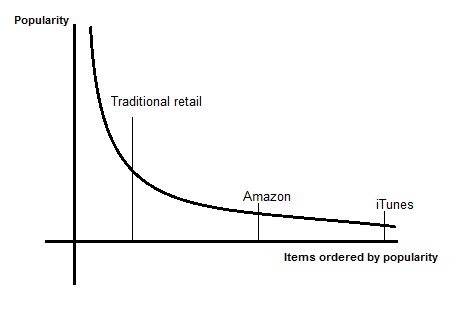
\includegraphics[width=250px]{img/longtail}%
	\end{center}
	\caption{The long-tail: Items ordered by popularity are layed out against their popularity rating. Most of the items reside in the long tail of the graph. Companies such as Amazon can offer a vastly greater subset of the total item space.}%
	\label{figure:longtail}%
\end{figure}

Typical applications of recommender systems are product recommenders for online retailers, movie and music recommenders such as \emph{Netflix}\footnote{\url{http://www.netflix.com/}} and \emph{Last.fm}\footnote{\url{http://www.last.fm/}}, and news article recommenders in online news services\cite{levy:2010, rajaraman:2012, celma:2008:phd}.


\subsection{Properties of recommender systems}\label{chapter:literature_study:section:computer:subsection:properties}

In \cite{herlocker:2004:ECF:963770.963772} and \cite{shani:2011:9780387858197}, Herlocker et al. and Shani et al.  respectively, compare the performance of recommender systems. A number of metrics for recommendation algorithms are described among which the following properties are listed. We will also describe methods for testing these properties, as described in \cite{shani:2011:9780387858197}.

\begin{itemize}
	\item \textbf{Accuracy}: The accuracy of item recommendations. There are three broad classes of prediction accuracy measures:
	\begin{itemize}
		\item the prediction of the rating given by a user;
		\item the prediction whether or not a user will actually use the item (for example adding to a queue) opposed to predicting the rating itself;
		\item the prediction of a ranking among items rather than an explicit rating of each item independently.
	\end{itemize}
	This kind of property is typically tested through an offline test on a training set, where parts of the recorded user profiles are hidden. The accuracy of the recommender system can then be determined by comparing the found recommendations to the remainder of the user profiles.
	\item \textbf{Novelty}: Novel recommendations are recommendations for items that the user did not know about. In a user study, users can be asked whether or not recommendations were new to them.
	\item \textbf{Serendipity}: Serendipity is a measure of how surprising the successful recommendations are. One can think of serendipity as "the amount of relevant information that is new to the user in a recommendation, or alternatively as deviation from the 'natural' prediction"\cite{shani:2011:9780387858197}. Serendipitous recommendations usually carry a higher risk, as they fall further from the class of known preferences. To find out the serendipity of recommendations, users can be asked directly if the recommendation was unexpected.
	\item \textbf{Diversity}: Diversity is generally defined as the opposite of similarity. To measure diversity content-based approaches can be used that compare recommended items.
	\item \textbf{Coverage}: One way to define coverage is the percentage of all items that are recommended to users during an experiment. Note that the cold start problem relates to coverage as it measures the coverage for a specific type of users, namely new users.
\end{itemize}

Many of these properties are closely related, as diverse recommendations that have a high coverage are likely to be serendipitous and novel. Also tradeoffs exist between properties; for example accuracy may drop as recommendations become more diverse\cite{shani:2011:9780387858197}. Looking at the Long-tail phenomenon, coverage, serendipity, novelty and diversity tend to be important. In the context of music recommendation, users usually want to find new music\cite{levy:2010}.


\subsection{A classification of recommendation algorithms}\label{chapter:literature_study:section:computer:subsection:algorithms}

Based on classifications presented in \cite{burke:2002} and \cite{celma:2008:phd}, a categorization of different types of recommendation strategies can be identified. We will only discuss the two most prominent ones, namely collaborative filtering (CF)\index{recommendation algorithm!collaborative filtering} and content-based filtering (CB)\index{recommendation algorithm!content-based filtering}\cite{herlocker:2000, rajaraman:2012}, and list some hybrid strategies. In the literature on recommender systems other general approaches that are commonly identified, are utility-based filtering, knowledge-based filtering, demographic filtering, and expert-based filtering\cite{bostandjiev:2012, burke:2002, song:2012}.


\subsubsection{Collaborative recommendation}\label{chapter:literature_study:section:computer:subsection:algorithms:subsubsection:cf}

\emph{Collaborative recommendation}\index{collaborative recommendation|see{collaboratibe filtering}} aggregates item ratings by users. By establishing overlaps between ratings in the corresponding user profiles, the system generates new item recommendations\cite{burke:2002, herlocker:2000}. User profiles consist of a vector of items and their ratings, which are continuously updated as the user interacts with the system over time\cite{burke:2002}.

For CF-based recommendation\index{CF|see{collaborative filtering}}, there are two classes of entities: users $U$ and items $I$. The data itself can then be represented by a utility matrix\index{utility matrix} $A$. The entries $a_{i,j}$ of the utility matrix represent what is known about the degree of preference of user $u_{i}$ and item $i_{j}$\cite{rajaraman:2012}. As can be seen in figure \ref{figure:utilitymatrix}, the utility matrix will have many blanks as well. The goal of the recommendation algorithm is then to fill in the blanks\cite{rajaraman:2012}.

\begin{figure}%
\begin{center}
	\includegraphics[width=250px]{img/utility_matrix}%
\end{center}
	\caption{The utility matrix $A$.}%
	\label{figure:utilitymatrix}%
\end{figure}

% Similarity / distance functions ...
In order to calculate the blanks, there is a variety of similarity functions that has been developed, e.g. \emph{cosine distance}, \emph{Pearson correlation}, \emph{Tanimoto-Jaccard}\cite{Verbert:2011:DRI:2090116.2090122}. For example, a small cosine distance will most likely correspond to a high similarity between profiles\cite{rajaraman:2012}. The discussion of the mathematics behind each of the algorithms is beyond the scope of this thesis.


\subsubsection{Content-based recommendation}\label{chapter:literature_study:section:computer:subsection:algorithms:subsubsection:cbf}

\emph{Content-based recommendation}\index{content-based recommendation|see{content-based filtering}} learns a profile of the user's interests based on the features present in objects the user has rated. New recommendations can then be generated based on a similarity function on these features\cite{burke:2002, pazzani:2007:CRS:1768197.1768209}.

When applying content-based filtering, the choice of similarity or classification function will have a significant impact on the quality of the recommendations. More importantly though, is the choice of features. To ensure good performance, these features should also be extracted easily from large quantities of data.

Depending on the type of item that is being recommended, different approaches can be applied to extract features and construct \emph{feature vectors}\index{feature vector}. Textual information is often extracted using a technique called \emph{stemming}\index{stemming} that uses root forms capturing a common meaning behind groups of words. Tuples of root forms and \emph{TF.IDF}, i.e., term frequency times inverse document frequency\index{TF.IDF}\index{term frequency times inverse document frequency|see{TD.IDF}}\nomenclature{TD.IDF}{term frequency times inverse document frequency} scores are computed for each word\cite{pazzani:2007:CRS:1768197.1768209, rajaraman:2012}. The words with the highest scores are the words that characterize the document\cite{rajaraman:2012}. A downside of stemming is that the process may cause the loss of contextual information for each word\cite{pazzani:2007:CRS:1768197.1768209}.

In \cite{bostandjiev:2012} and \cite{melville:2002:CCF:777092.777124} web crawlers are used to gather and extract features from online documents. Each property or feature is a 'bag of words'\index{bag of words} that can be used in a naive Bayesian text classifier\index{Bayesian classifier}. This way each item can be categorized and the profile can be 'learned'\cite{melville:2002:CCF:777092.777124}.

\emph{Tags}\index{tag} are very useful as well. Although they can be generated from text, for complex objects such as images and music, tag generation relies on user input\cite{rajaraman:2012}. Nonetheless, emerging technologies such as the 'search by image' option introduced by \emph{Google}\footnote{\url{http://www.google.be/imghp?hl=nl&tab=Ti}}, allow to retrieve web sites, documents and key words related to the given image\cite{google:2011:afbeeldingen}.

Mathematical models for music also allow for feature extraction. Algorithms have been developed to classify music based on content features\cite{Li:2006:TIM:2219090.2219562, tzanetakis:2002}. There are various types of acoustic features that can be extracted. In \cite{Li:2006:TIM:2219090.2219562} a distinction is made between rhythmic content features, pitch content features and timbral content features.


\subsubsection{Hybrid recommendation}\label{chapter:literature_study:section:computer:subsection:algorithms:subsubsection:hf}

\emph{Hybrid filtering}\index{hybrid filtering} combines two or more recommendation algorithms\cite{burke:2002}. In \cite{burke:2002} a number of hybrid recommendation strategies are discussed. Robin Burke lists seven different approaches for combining recommendation algorithms. Each of these combinations also has its advantages and disadvantages. Not necessarily all combinations will be successful, and not all of them have been implemented\cite{burke:2002}.

A good hybrid model is likely to outperform any single approach, as weaknesses of one strategy may be cancelled out by the advantages of another\cite{song:2012}.

%Hybrid systems for music recommendation can be built that use both collaborative filtering approaches and content-based approaches.



\subsection{Challenges for recommender systems}\label{chapter:literature_study:section:computer:subsection:challenges}

Each recommendation technique has benefits as well as drawbacks. Some of these apply to all or most types of recommendation strategies, while others are only relevant to certain cases.

The \emph{cold start} and \emph{gray sheep} problem both affect prediction accuracy. The \emph{black box} problem is more closely related to perceived accuracy and trust in the recommender system.


\subsubsection{Cold start}

Both CF and CB-based recommendation algorithms suffer from the ramp-up\index{ramp-up|see{cold start}} problem in one way or the other. The 'ramp-up' or 'cold start' problem\index{cold start} (although they may refer to slightly different problems depending on the literature) is dual problem that encompasses two distinct, yet related problems as defined in \cite{burke:2002}:

\begin{itemize}
	\item \textbf{New User}\index{cold start!new user}: Finding recommendations for users with a limited rating history is hard. Since user profiles tend to build up over time, new users usually fall in this category. As a result, recommender accuracy tends to be lower for new users.
	\item \textbf{New Item}\index{cold start!new item}: A new item will most likely not have that many ratings associated with it, and as a result will not be easily recommended. This 'new item problem' typically emerges when new items are constantly added to the system; for example when browsing a constant stream of news articles. When new articles are introduced, not many users have had the chance yet to rate these items. In the case of a news feed, an additional problem is that these items are short-lived, meaning that at some point these item profiles will most likely stop receiving any ratings at all.
\end{itemize}

Both of these issues translate themselves into a sparse regions in the utility matrix. It is worth noting that content-based recommendation algorithms suffer less from the \emph{new item} problem, as these tend to rely on features that are inherent to the items themselves, rather than user generated content. This is one of the reasons hybrid approaches can provide a solution to collaborative filtering\cite{burke:2002}. For example, in \cite{melville:2002:CCF:777092.777124}, content-based predictors are used to create pseudo-user ratings to reduce sparsity of the utility matrix, used in a collaborative algorithm.


\subsubsection{Gray sheep}

A problem that is typical of collaborative filtering is the 'gray sheep problem'\index{gray sheep}\cite{burke:2002, herlocker:2000}. The gray sheep problem occurs when a user falls between different clusters of users that may have contradicting item ratings. As a result, it is hard to determine how to classify the user\cite{burke:2002}.

Classifying users is typically a harder problem than classifying artists. An artist can usually be classified into one particular genre, whereas two users may have one genre in common, but may have rather conflicting tastes as well\cite{rajaraman:2012}.

% Having a lot of users will increase the likelyhood of finding similar users, even if a user has a broad taste. \emph{IMDb}\footnote{http://www.imdb.com} shows statistics of similar users, and \emph{Last.fm} allows to browse neighbouring profiles.


\subsubsection{Black box}

Another issue with recommendation systems is that these system often appear as 'black boxes' towards the end user\index{black box}. The complexity of the algorithms used, prevents the user from understanding the recommendation rationale\cite{zhao:2010}. This problem may decrease the acceptance by the user of item suggestions. One of the solutions for this problem, proposed by Herlocker et al. in \cite{herlocker:2000}, is to provide an explanation system, i.e., the white box\index{white box}, on top of the recommender system that explains the recommendation process. This can be done through providing a transcript of the system's reasoning or through visualizations\cite{herlocker:2000}.

In this thesis we will focus mainly on this problem. We will look at the black box problem in the context of collaborative music recommendation, and try to design, implement and test a new visual explanation system in an effort to overcome this problem.


\subsection{Music recommendation}\label{chapter:literature_study:section:computer:subsection:music}

%A number of popular recommender systems for music exist. For example Last.fm, Spotify, Grooveshark, Deezer are specifically aimed at music recommendation, but also websites such as Facebook, Youtube, and Amazon have can provide recommendation for music. Most of these systems use collaborative filtering, sometimes in combination with content-based features.

\subsubsection{Examples}

A number of popular recommender systems for music exist, such as \emph{Last.fm}\footnote{\url{http://www.last.fm/}}, \emph{Spotify}\footnote{\url{http://www.spotify.com/}}, \emph{Grooveshark}\footnote{\url{http://www.grooveshark.com/}}, \emph{Deezer}\footnote{\url{http://www.deezer.com/}}, \emph{Tastekid}\footnote{\url{http://www.tastekid.com/}}, \emph{Pandora}\footnote{\url{http://www.pandora.com/}} and so on.

\emph{Last.fm} is an example of a music recommender system that is based on the collaborative filtering\cite{levy:2010}, although it uses additional content-based approaches as well\cite{song:2012}. Also \emph{Pandora}, \emph{Allmusic}\footnote{\url{http://www.allmusic.com}} and \emph{Shazam}\footnote{\url{http://www.shazam.com}} use hybrid approaches\cite{song:2012}.

Bostandjiev et al. \cite{bostandjiev:2012} have built a music recommender\index{TasteWeights} that uses \emph{Wikipedia}\footnote{\url{http://www.wikipedia.org/}}, a content-based source, \emph{Facebook}\footnote{\url{https://www.facebook.com/}}, a collaborative source, and \emph{Twitter}, an \emph{expert-based!recommender algorithm}\index{expert-based!recommender algorithm} or \emph{context-based}\index{context-based} source.

\subsubsection{Profile generation}

One of the difficulties for any recommendation algorithm is the modeling of good user and item profiles. Song et al. \cite{song:2012} list several approaches for music recommendation.

A typical \emph{user profile} exists out of two types of data: a collection of demographic, geographic and/or psychologic data, and user listening experience\cite{song:2012}.

Music libraries are often constantly changing, as new music is added to the user profile, listening patterns change and listening history is updated. As a result, music recommenders should be able to address this kind of \emph{dynamic evolvement}\index{dynamic evolvement}\cite{song:2012}. For example, \emph{Last.fm} deals with this problem through their \emph{Scrobbler}, which tracks the user's listening history through various media players\cite{lastfm:2013:scrobbling}.

In \cite{song:2012} three types of data are associated with \emph{item profiles}:

\begin{itemize}
	\item \textbf{Editorial metadata} (EM)\nomenclature{EM}{editorial metadata}\index{editorial metadata}: for example composer, performing artist, title, genre, cover art, et cetera.
	\item \textbf{Cultural metadata (CM)}\nomenclature{CM}{cultural metadata}\index{cultural metadata}: data obtained from analysis of text-based sources, enabling a categorization of music; for example tag-based feature extraction as described in section \ref{chapter:literature_study:section:computer:subsection:algorithms:subsubsection:cbf}.
	\item \textbf{Acoustic metadata (AM)}\nomenclature{AM}{acoustic metadata}\index{acoustic metadata}: data directly obtained from analysis of audio signals; for example wavelet-based approaches described section \ref{chapter:literature_study:section:computer:subsection:algorithms:subsubsection:cbf}.
\end{itemize}

As described in section \ref{chapter:literature_study:section:computer:subsection:algorithms:subsubsection:cbf}, item profiles can be used for content-based item recommendation.














% ------------------------ The interface --------------------------
% 
% -----------------------------------------------------------------
\section{Information visualization}\label{chapter:literature_study:section:interaction}

% What will we study?
% Link with previous sections?

In this section different aspects of information visualization that were used to visualize the recommendation rationale are highlighted. First types of data are discussed, next we will look at visual encodings for these types of data. Finally we will discuss some visualization, interaction and data reduction techniques that were used in the \emph{SoundSuggest} application.


\subsection{Types of data}\label{chapter:literature_study:section:interaction:subsection:datatypes}

% context
% wat can be visualized, data types (recommender data)

Information visualization\index{information visualization}\index{infovis|see{information visualization}} has been focusing on on data sets that lack inherent spatial semantics, thus posing a challenge to map the abstract data onto a two-dimensional screen space\cite{keim:2002}. Within this category of data, still different types of data can be distinguished and their characteristics will have an influence on the type of visualization.

\emph{Tables of data} consist out of rows, representing items, and columns, representing the data dimensions, or 'attributes'. The number of dimensions is referred to as the dimensionality\index{dimensionality} of the data set\cite{keim:2002}. There are three different kinds of dimensions, namely\cite{shirley:2009}:

\begin{itemize}
	\item \textbf{Quantitative}: numerical data on which arithmetic can be applied. For example playcount of a particular track, the duration of a track, the number of artists that two users have in common, et cetera. Quantative data occurs in all kinds of music and user metadata.
	\item \textbf{Ordered}: an enumeration that has a definite order. For example ratings such as 'good', 'average', and 'bad'.
	\item \textbf{Categorical}: data that has no specific ordering, and is distinguished by name only. For example composer names, band members, artist tracks, users who like a particular item, et cetera. Most editorial and cultural metadata can be considered categorical.
\end{itemize}

In the utility matrix each column corresponds to an item and a row to a user. The entries of this matrix are typically quantitative data, while item and user names are categorical data.

\emph{Relational data}\index{relational data} on the other hand consists out of nodes\index{graph!node} and links or 'edges'\index{graph!edge}\cite{keim:2002, shirley:2009}. Both nodes and edges can have associated attributes. These attributes can again be either of quantitative, ordered, or categorical nature.

The underlying structure of collaborative filtering, the utility matrix, can be interpreted as a \emph{dual graph}\index{dual graph}. This is a graph $G(V,E)$ for which $V = U \cup I$ such that $U \cap I = \emptyset \wedge E \subseteq U \times I$\cite{dekimpe:2007}. Each non-blank entry in the utility matrix will then correspond to an edge. Figure \ref{figure:dualgraph} shows the dual graph of the corresponding utility matrix.

When applied to the context of collaborative filtering, the set of nodes $U$ corresponds to the set of users, and the other set of nodes $I$ is set of items. In conclusion this means that there only exist edges of that go from an item to a user or from a user to an item.

\begin{figure}%
	\begin{center}
		\includegraphics[width=300px]{img/dualgraph}
	\end{center}
	\caption{Transforming the utility matrix into a dual graph: two distinct sets of nodes, users and items, only share edges between nodes of different sets.}%
	\label{figure:dualgraph}%
\end{figure}




\subsection{Visual encoding and visual channels}\label{chapter:literature_study:section:interaction:subsection:encoding}

%Visual encoding principles

\emph{Visual encoding}\index{visual encoding} is defined as the mapping of data set attributes to a visual representation. The choice of visual encoding is one of the central problems in the visualization design\cite{shirley:2009}.

Visual encoding takes place through \emph{visual channels}\index{visual channel}. A visual encoding corresponds to a graphical element, or 'mark'. Examples of visual channels are spatial position, color, size, et cetera. The dimension of the mark may vary: a point is a zero-dimensional mark, a line a one-dimensional one, an area a two-dimensional one and so on.

A visual encoding has the following characteristics, as described in\cite{shirley:2009}:

\begin{itemize}
	\item \textbf{Distinguishability}: the ability of a user to distinguish between visual encodings;
	\item \textbf{Seperability}: Separable visual channels are opposed to integral visual channels, which are focused together on a pre-conscious level. Separable visual channels are safe to use for encoding multiple dimensions;
	\item \textbf{Pop-out}: selecting a channel and make it visually stand out from all the others.
\end{itemize}

%Visual channels

There is a variety of possible visual channels that a visualization designer can turn to in order to create a visual encoding, such as colour, spatial position, size, shape, orientation, and so on. The performance of the visual encoding (through a visual channel) depends on the type of data, i.e. quantitative, ordered or categorical \cite{shirley:2009}. Figure \ref{figure:encodings} gives an overview of the performance for each category, adapted from \cite{shirley:2009}. Note that spatial position is the most accurate for each data type\cite{shirley:2009}.

%Figure 1: Visual encoding performance for each data type
\begin{figure}%
	\begin{center}
		\includegraphics[width=250px]{img/visualencodings}%
	\end{center}
	\caption{Visual encoding performance for each data type, ordered from best to worst.}%
	\label{figure:encodings}%
\end{figure}


\subsubsection{Colour}

In \cite{shirley:2009} colour is considered in terms of three separate channels: \emph{hue}, \emph{saturation} and \emph{brightness}. This allows for different encodings. Just like for most visual channels, the choice of the channel (hue, saturation or brightness) depends heavily on the type of data.

For categorical data, hue can be successfully applied, keeping in mind its small range. As a rule of thumb, a maximum of eight hue categories should be used in a visualization. An important remark is that roughly 10\% of men is red-green color deficient. If a coding uses red and green, it may be wise to apply redundant coding using lightness or saturation in addition to hue \cite{shirley:2009}.

In the \emph{SoundSuggest} application, items in a list of neighbours are highlighted using the hue visual channel to distinguish between three different groups of items.


\subsubsection{Spatial layout}

Spatial layouts form other visual channels. Although these tend to be the most accurate, spatial layouts in two and three dimensions have several weaknesses; two of these are\cite{shirley:2009}:

\begin{itemize}
	\item \textbf{Occlusion}: Parts of the data set become hidden by others. In the case of the mapping of abstract dimensions onto spatial positions, understanding the details of a three-dimensional visualization may be challenging, even if the user is allowed to change viewpoints. For the \emph{SoundSuggest} application, elements in the vsiualization may overlap when edges cross.
	\item \textbf{Text in arbitrary orientations}: Special care has to be taken with text, as it may become very hard to read depending on the orientation. In the \emph{SoundSuggest} application artist names are turned according to their position on the circle layout.
\end{itemize}

% text problem: try to overcome: click --> shows title

To overcome limitations of visual channels, various visualization, interaction, and data reduction techniques may be applied\cite{keim:2002, shirley:2009, ware:2004}. Before discussing this any further, the following section will first take a closer look at graph drawing.



\subsection{Graph-based visualization}\label{chapter:literature_study:section:interaction:subsection:graphs}

Relational data\emph{relational data} is data that has an inherent relation among its elements\cite{shirley:2009}. The graph drawing problem describes the problem of how nodes and edges are visualized on a display\index{graph drawing problem}\cite{herman:2000}.

Scalability is one of the central issues with graph drawing, as graph size poses several important challenges\cite{herman:2000}. The following issues are of course closely related to the general problems of visualization design discussed in section \ref{chapter:literature_study:section:interaction:subsection:encoding}:

\begin{itemize}
	\item \textbf{Viewability and discernability}: even if it is possible to layout and display all the elements, it may become impossible to discern between nodes and edges;
	\item \textbf{Performance and responsiveness}: graph layout algorithms may be relatively complex, and a large number of nodes and edges may become a bottleneck for performance, especially in interactive applications that require reasonable responsiveness;
	\item \textbf{Usability}: apart from problems with discernability, also information overload may occur. It is known that detailed analysis of data in graph structures is easiest when the displayed graph is small.
\end{itemize}


As graph size is one of the biggest issues of graph visualization, techniques have been developed to apply data reduction techniques on graphs\cite{herman:2000, shirley:2009}. Apart from the traditional distortion and data transformation techniques, there are some techniques that are specific for graph-based visualization.

\subsubsection{Data and dimensionality reduction}

Based on a visualization design by Valdis Krebs in \cite{steele:2010}, a dimensionality reduction\index{dimensionality reduction} can be performed on the dual graph, by keeping only one set of nodes and representing the other set of nodes as implicit information in the edges. Figure \ref{figure:rowreduction} shows an example of this idea of 'row reduction'\index{row reduction}. In Krebs' visualization the items, books purchased from the Amazon web store in this case, were retained. In the resulting graph, two items would share an edge if a user bought both these items. The thickness of the edges represented the number of users that where linked to these items\cite{krebs:2012:networkthinkers, steele:2010}.

\begin{figure}%
	\begin{center}
		\includegraphics[width=250px]{img/row_reduction}%
	\end{center}
	\caption{A row reduction operation on each pair of edges in a dual graph will result in a dimensionality reduction where one set of nodes is removed from the graph. An additional data reduction can be achieved by clustering edges into a thicker edge. Edge thickness then depends on the number of edges involved.}%
	\label{figure:rowreduction}%
\end{figure}

The \emph{SoundSuggest} application does not use the final step of Krebs' graph design. Instead parallel edges are retained to keep a direct link between user and edge. In the resulting visualization of the CF-based recommender, a quantification of the similarity between users can then be established by counting parallel edges between items that occur in neighbouring profiles. Figure \ref{figure:rowreduction_dualgraph} shows how the dual graph from figure \ref{figure:dualgraph} is transformed into a circular graph layout with the remaining item nodes, similar to the visualization in figure \ref{figure:hierarchical_edge_bundling}.

\begin{figure}%
	\begin{center}
		\includegraphics[width=250px]{img/dualgraph_rowreduction}%
	\end{center}
	\caption{Row reduction applied on the graph in figure \ref{figure:dualgraph}.}%
	\label{figure:rowreduction_dualgraph}%
\end{figure}

As it is unlikely that the whole user profile can be shown in the graph while avoiding visual clutter, the active user's favourite items are used to give a representation of the active user's profile. This way the user can still directly compare him/herself with neighbouring profiles.


\subsubsection{Clutter reduction}

Based on a survey by Herman et al. \cite{herman:2000}, and papers by Holten \cite{Holten:2006:HEB:1187627.1187772}, and Holten et al. \cite{holten:2009}, the following gives an brief overview of two techniques: \emph{clustering}\index{clustering} and \emph{edge-bundling}\index{edge-bundling}.

\emph{Clustering}\index{clustering} is the process of discovering groupings or classes in data based on chosen semantics, i.e., structure, or content. An example of structure-based approach is to bundle groups nodes that have certain number of edges between them. For content-based approaches, edges or nodes with similar attribute values can be clustered.

Due to the sparsity of the utility matrix, we might have to cluster multiple neighbouring profiles in a single node to ensure adequate connectivity within the resulting graph.

\emph{Edge-bundling}\index{edge-bundling} is a technique to visualize compound graphs\cite{Holten:2006:HEB:1187627.1187772}. Edges are modelled as "flexible springs that can attract each other, similar to how electrical wires are bundled within a network"\cite{holten:2009}. Figure \ref{figure:hierarchical_edge_bundling} gives an overview of the different results for varying bundling strengths. It shows how edges are drawn closer towards each other, reducing visual clutter, and highlighting relationships between nodes.


% BEGIN FIGURE : hierarchical_edge_bundling
\begin{figure}
	\centering
	\begin{subfigure}[b]{0.3\textwidth}
					\centering
					\includegraphics[width=\textwidth]{img/hierarchical_edge-bundling1}
					\caption{Low edge bundling strength.}
					\label{figure:hierarchical_edge-bundling1}
	\end{subfigure}%
	~
	\begin{subfigure}[b]{0.3\textwidth}
					\centering
					\includegraphics[width=\textwidth]{img/hierarchical_edge-bundling2}
					\caption{Medium edge bundling strength.}
					\label{figure:hierarchical_edge-bundling2}
	\end{subfigure}
	~
	\begin{subfigure}[b]{0.3\textwidth}
					\centering
					\includegraphics[width=\textwidth]{img/hierarchical_edge-bundling3}
					\caption{High egde bundling strength.}
					\label{figure:hierarchical_edge-bundling3}
	\end{subfigure}
	\caption{Hierarchical edge bundling. Taken from \url{http://mbostock.github.io/d3/talk/20111116/bundle.html}. By increasing the bundling strength, edges will be drawn towards each other, clearly marking pathways between endpoints.}%
	\label{figure:hierarchical_edge_bundling}%
\end{figure}


Figure \ref{figure:edgebundling_dualgraph} shows how this can be applied on the graph from figure \ref{figure:rowreduction_dualgraph}. From a graph drawing perspective we managed to reduce visual clutter by reducing the number of displayed items and applying edge-bundling\cite{herman:2000, Holten:2006:HEB:1187627.1187772}.

\begin{figure}%
	\begin{center}
		\includegraphics[width=250px]{img/dualgraph_edgebundling}%
	\end{center}
	\caption{Edge bundling applied on the graph in figure \ref{figure:rowreduction_dualgraph}.}%
	\label{figure:edgebundling_dualgraph}%
\end{figure}










%The term 'human-computer interaction' describes a phenomenon where two actors, the human or \emph{user} and the computer or \emph{system}, share a communication channel. The communication channel is a representation of data of the system towards the user. It is clear that both actors will impose certain restrictions on this visual communication channel\cite{shirley:2009, ware:2004}. In this chapter we will try to establish who these actors are, what this communication channel looks like, and what kind of restrictions are imposed upon the visual communication channel. 

% --------------------------- The User ----------------------------
% 
% -----------------------------------------------------------------
\section{Gaining insight into interactive visualization}\label{chapter:literature_study:section:user}

The goal of the \emph{SoundSuggest} application is to allow the user to gain insight into the system through an interactive, visual explanation system. Two specific questions arise:

\begin{itemize}
	\item how does a human gain insight?
	\item are there any human limitations imposed on the design of an interactive visualization?
\end{itemize}

The following subsections try to establish an answer to these questions. Most of the ideas in these subsections are drawn from papers by Yi. et al. \cite{yi:2008}, Chris North \cite{north:2006}, Klein et al. \cite{Klein:2006:MSS:1158821.1159015, klein:2006:MSS:1175882.1176017}, and a book by Colin Ware \cite{ware:2004}.










% --------------------------- The User ----------------------------
% INSIGHT
% -----------------------------------------------------------------
\subsection{Insight gaining}\label{chapter:literature_study:section:user:subsection:insight}

In \cite{north:2006} it is argued that insight\index{insight} is not a well-defined term. A formal definition might be too restrictive to capture its essence, and yet too broad to be useful. To quantify insight, \cite{north:2006} and \cite{yi:2008} list characteristics that allow a finer evaluation:

\begin{itemize}
	\item \textbf{Complex}: insight is complex in the sense that it involves large amounts of data, cf. the input data of a recommender system, that form cognitive constructs, rather than individual units.
	\item \textbf{Deep}: insight is self-generating in a way, as insight provides a starting point for insight on the next level. Users may apply previously gained insight into a certain recommendation on other recommendations.
	\item \textbf{Qualitative}: insight is subjective, uncertain and can have multiple levels of resolution;
	\item \textbf{Unexpected}: insight is usually unpredictable, serendipitous and creative;
	\item \textbf{Relevant}: insight is deeply embedded in the data domain: it gives data meaning as it connects data to the existing domain knowledge: the user has to give meaning to seeminly random suggestions.
\end{itemize}

The quality of insight can then be determined by quantifying each of these characteristics\cite{north:2006}. North describes methods to evaluate insight gaining through visualizations, such as usability testing, heuristic evaluation, cognitive evaluation, and controlled experiments on benchmark tasks\cite{north:2006}.

Chris North notes that controlled experiments suffer from four fundamental problems that may hinder effective evaluation of previously listed characteristics of insight. Such experiments are\cite{north:2006}:

\begin{itemize}
	\item \textbf{Predefined}: Following specific, predefined instructions leave little room for unexpected insight.
	\item \textbf{Limited in time}: Short task times leave little room for deep insight.
	\item \textbf{Definitive}: Multiple choice questions leave little room for quantative insight.
	\item \textbf{Superficial}: Answers are concise, leaving little room for complex and relevant insight.
\end{itemize}

In this thesis we will focus on the think aloud technique instead. This is part of an alternative method described by Chris North that includes three key innovations\cite{north:2006}:

\begin{itemize}
	\item an open-ended protocol;
	\item a qualitive insight analysis;
	\item an emphasis on domain relevance.
\end{itemize}

In this technique users are free to explore the data. By applying the think aloud protocol, the user's insight's can be captured. In order to increase domain relevance, the test users should be users from the target audience. Domain experts can then provide "a critical metric for the value of importance of the reported insights in the domain"\cite{north:2006}.


\subsubsection{Sensemaking}\label{chapter:literature_study:section:user:subsection:insight:subsubsection:sensemaking}

\emph{Sensemaking}\index{sensemaking} plays an important part in insight gaining \cite{yi:2008}. The definitions for sensemaking may vary. We adapt the definition presented by \cite{Klein:2006:MSS:1158821.1159015} and \cite{yi:2008}.

In \cite{Klein:2006:MSS:1158821.1159015} sensemaking is looked at from a psychological perspective, a perspective of human-centered computing, and the perspective of naturalistic decision making. Sensemaking is then defined as follows: "sensemaking is a motivated, continuous effort to understand connections in order to anticipate their trajectories and act effectively"\cite{Klein:2006:MSS:1158821.1159015}.

Based on the discussion in \cite{klein:2006:MSS:1175882.1176017} and \cite{yi:2008}, Soo Yi et al. describe the process of sensemaking. Sensemaking is a:

\begin{itemize}
	\item \textbf{Cyclic and iterative proceduce}: consisting out of a generation loop searching for representations, a data coverage loop instantiating the representations and finally shift representations;
	\item \textbf{Creation procedure}: being more about reasoning than discovery;
	\item \textbf{Retrospective procedure}: as people construct a framework and assign relevant information to a place withing this framework. If the data fits the framework well, the framework is confirmed, otherwise it may be updated or discarded;
\end{itemize}

An important remark made in \cite{Klein:2006:MSS:1158821.1159015} is that data fusion algorithms can reduce information overload, but they also pose challenges to sensemaking if the human can't form an accurate mental model of the machine, to understand why and how the algorithms are doing what they are doing.

%The recommender system's algorithm may use weights, clustering and other techniques. A particular explanation system may not describe the recommendation process with such detail. Also, the data visualized by an explanation system may cover a much smaller subset of the actual data that was processed to compute a particular recommendation. When working with large sets of data, like in the case of a recommender system, clustering, glyphs, dimensionality reduction and other data fusion techniques may be applied to describe a multitude of data units in a single visual entity\cite{herman:2000, keim:2002, shirley:2009, ware:2004}.

The data and dimensionality reduction algorithms used in \emph{SoundSuggest}, increase the amount of implicit information that needs to be interpreted by the end user\cite{herman:2000, ware:2004}. In order to gain insight into the recommendation process, it is important that certain contextual information is retained. The contextual information we want to convey is two-fold:

\begin{enumerate}
	\item The strength of the links between a recommendation and the user's profile;
	\item The position of the user in his/her neighbourhood and the relation with those neighbours.
\end{enumerate}

% interaction techniques
The first type of information is contained in parallel edges between items. For the second type of information, the active user's neighbours should be included in the visualization in one way or the other. In the resulting visualization the user's top neighbours are listed next to the graph. By hovering or clicking one of the listed neighbours, the relevant parts of the graph, i.e., items owned by the neighbour and the edges between them, are highlighted.



\subsubsection{Processes of insight gaining}\label{chapter:literature_study:section:user:subsection:insight:subsubsection:processes}

Although sensemaking can play an important part in gaining insight, it is not the only path to arrive at insight \cite{yi:2008}. Yi et al. \cite{yi:2008} identify four processes, that are often intertwined, through which insight is established:

\begin{itemize}
	\item \textbf{Provide overview}: \textit{In this process the individual gains understanding of the big picture of a dataset of interest. It allows the user to make a distinction between what is known to him/her and what is not.} The user gets an overview of the recommendation rationale.
	\item \textbf{Adjust}: In this process a person will explore a dataset by adjusting the level of abstraction and/or the range of selection. Typical actions involve filtering and grouping of data.
	\item \textbf{Detect pattern}: \textit{In this process the user will try to identify specific distributions, trends, frequencies, outliers or structure in the dataset.} Through numerous interactions, the user is able to identify a pattern in the relationshpis between recommendations.
	\item \textbf{Match mental model}: In this process the gap between data and cognitive model is bridged, reducing cognitive load and linking the present visual information with real-world knowledge.
\end{itemize}

The link with sensemaking is found in the cyclic and iterative nature of sensemaking - provide overview, adjust and detected pattern can be applied iteratively, as well as its creative and retrospective aspects - adjust and detect pattern create hypotheses and test them through various interaction techniques\cite{yi:2008}.

It would be interesting to see if we can identify these steps in the user tests performed in this thesis as well.


\subsubsection{Improving insight}\label{chapter:literature_study:section:user:subsection:insight:subsubsection:improving}

% !!!!!!!
% + explain how used in the application

Yi et al. \cite{yi:2008} identify several ways in which the insight gaining process can be made more efficient. They list the system's interactivity, the quality of visual encodings and usability among others, as possible enablers for increased insight gaining. Naturally, careless designs will act as barriers rather than enablers in the insight gaining process.

% careless, improvident, nonchalant, ...

Interactivity of the system promotes the user's engagement into the dataset. Spending more time with the data will allow users to form more detailed and accurate hypotheses, and as a result greater insight\cite{yi:2008}. At the same time, while using the visualization, the user will become more skilled at a task over time. Nonetheless, bare in mind that when performing long and tedious search tasks, vigilance will become an important aspect as well in the efficiency of data exploration\cite{ware:2004}. Visual explanation systems may involve interaction techniques. For example, in the \emph{SoundSuggest} application, users can click an item node. Related item nodes will then be highlighted with it as well. An important consideration is that the interval between the human action and the result on the screen should be low, promoting the so-called \emph{priciple of transparency}\index{priciple of transparency}. The objective of transparency is that the user will have the illusion of directly manipulating the data on the screen.

Similarly visual encodings that are counter-intuitive will also increase the cognitive load. Other barriers on insight gaining are clutter, occlusion and data overload\cite{yi:2008}. In the application we have built, we applied clutter reduction techniques for graph visualization.

Usability is another aspect that may have an impact on the insight gaining process, as controls that are hard to use will inevitably occupy some of the cognitive capacity of the user\cite{yi:2008}. In the ISO standard ISO 9241-11, usability is defined as "the extent to which a product can be used by specified users to achieve specified goals with effectiveness, efficiency and satisfaction in a specified context of use"\cite{usabilitynet:2006:standards}.

Note that usability\index{usability} should not be considered a one-dimensional property of a user interface. Nielsen identifies several characteristics of usability in applications\cite{nielsen:1993:UE:529793}:

\begin{itemize}
	\item \textbf{Learnability}: if the system is easy to learn, the user can get started quickly;
	\item \textbf{Efficiency}: if the system is efficient to use, it will be possible to complete more work in less time;
	\item \textbf{Error rate and severity}: if the system should be robust and minimize faults;
	\item \textbf{Memorability}: once the system is learned, acquired skills should not be forgotten easily;
	\item \textbf{Satisfaction}: the system should be pleasant to use.
\end{itemize}

Note that an application may not necessarily have to have a high value for each of these properties. An expert visual explanation system that is highly complex may score low on learnability, while still remaining a very usable system. On the other hand, a system for casual users may require high learnability, otherwise users will be reluctant to use it. The application we have built is aimed at users that want to dig deeper into the recommendation data to gain a better understanding of the recommendation system's rationale, but without going into high detail.

One of the aspects of the user tests we conducted involved testing the perceived usability of the application through test questionnaires. Through the think aloud protocol described ealier, some usability problems could also be detected through observation.


















% --------------------------- The User ----------------------------
% INTERACTIVE VISUALIZATION
% -----------------------------------------------------------------
\subsection{Interactive visualization}\label{chapter:literature_study:section:user:subsection:interactive}

%As we now have a better understanding of what insight is, we will try to establish how the insight gaining process works through visual data mining\index{visual data mining} and interactive visualization\index{visualization!interactive visualization}.

The relation between insight gaining and data visualization has been pointed out in other research. Colin Ware \cite{ware:2004} describes interactive visualization as an "internal interface between the user and the computer in a problem solving system". Keim \cite{keim:2002} notes that "idea behind visual data exploration, is to present data in a visual form, allowing the user to gain insight into the data, draw conclusions, and directly interact with the data".

In a chapter on visualization\index{visualization} in \cite{shirley:2009}, Tamara Munzner describes visualization as follows: "visualization allows the user to offload cognition to the perceptual system, using graphical data representations as a form of external memory. Therefore, by augmenting human capabilities, the data analyst is aided to understand, explore and form hypotheses of the data"\cite{shirley:2009}. In conclusion, the \emph{visual data exploration}\index{visual data mining}\index{visual data exploration|see{visual data mining}} process can then be understood as a hypothesis generation process\cite{keim:2002}.

A reoccurring theme in visualization design is Schneiderman's mantra: "overview first, zoom and filter, and details on demand"\cite{keim:2002, shirley:2009, ware:2004}. First, the user looks for patterns of interest in the data space. Next the user focuses on one or more of these patterns, and starts looking at the data on a more detailed level. The user can then draw his/her conclusions and explore the data space further\cite{keim:2002}. 

In what follows, we try to describe how a human interacts with interactive visualization on a cognitive level. It will be clear that some parallels can be drawn with the insight gaining process. This should come as no surprise, since these processes are intertwined\cite{keim:2002, ware:2004, yi:2008}.

In \cite{ware:2004}, interactive visualization is characterized by three classes of feedback loops:

\begin{itemize}
	\item \textbf{Data selection and manipulation loop}: the user selects and moves objects that are selected through simple interactions based on eye-hand coordination;
	\item \textbf{Exploration and manipulation loop}: the user tries to find his/her way through a large visual data space;
	\item \textbf{Problem solving loop}: the user forms hypotheses about the data and refines them through an augmented visualization process.
\end{itemize}

The next subsections describe each feedback loop in greater detail.


\subsubsection{Data selection and manipulation loop}\label{subsubsection:data_manipulation_loop}

In the data selection and manipulation loop a user will try to interact with the visualization. For example by clicking a node in a graph, hovering a list of elements and so on. The quality of performance of selecting and manipulating data on a screen, depends on certain factors. Colin Ware discusses the following attributes:

\begin{itemize}
	\item \textbf{Reaction time}: This is the amount of time for a user to identify and select certain objects.
	\item \textbf{Types of interaction}: different types of interaction will have a different influence on user performance. In our visualization only two types of interaction are supported: clicking and hovering buttons, links or words.
	\item \textbf{Learning}: The speed at which a user performs a task may decrease over time, as the user becomes more skilled at executing the task.
\end{itemize}

Each of these attributes may be influenced by different factors. Through experiments predictions for these parameters have been captured in various laws such as Hick-Hyman law (reaction time), Fitt's law (selecting an object in a two-dimensional space) and the power law of practice (learning effects)\cite{ware:2004}. Based on these laws, it is expected that reaction time will decrease over time as users become more familiar with the visualization.


\subsubsection{Exploration and navigation loop}\label{subsubsection:exploration_navigation_loop}

In the second loop the user navigates through the data space. The basic navigation control loop is described as an iterative process that involves two distinct aspects\cite{ware:2004}:

\begin{itemize}
	\item \textbf{Human}: The user gains understanding of, i.e., gains insight into, the data space through a logical, spatial model. Parts of this model may be encoded in the longterm memory, on the condition that the data space is maintained for a long enough period of time.
	\item \textbf{Computer}: The visualization may be updated and refined based on user input. Through clicks and hover queries the user will be able to change parts of the visualization.
\end{itemize}

When exploring spatial maps, a user is confronted with the \emph{focus-context problem}\index{focus-context problem}, i.e., "the problem of finding detail in a larger context"\cite{ware:2004}. The objective is to see the relation between the larger context and the details, rather than finding details. Ware goes on to discern between spatial, structural and temporal scales in which the focus-context problem manifests itself\cite{ware:2004}.

Ware and Mitchell remark that the human visual system is already well-adapted to the spatial focus-context problem\cite{ware:2004}. Therefore, they argue that when designing a display, it should already try to take a maximal advantage of these perceptual skills. This can be done by displaying as much data as possible, without causing visual overload\cite{ware:2004}. Of course, there are always computational costs, either finding the best way to represent large amounts of data, or instead, using interaction techniques to delve deeper into the data\cite{herman:2000, shirley:2009}.

% cf. graph drawing problem vs. focus+context, e.g. fish-eye

%The time it takes to navigate between two points in the data space to gather information is called the \emph{cost of knowledge}\index{cost of knowledge}\cite{ware:2004}. To keep the cost of knowledge low, various interaction techniques have been developed, such as distortion, rapid zooming, elision, and multiple windows\cite{ware:2004}.


\subsubsection{Problem solving loop}\label{subsubsection:problem_solving_loop}

The problem solving loop can be described through means of a \emph{visual thinking algorithm}\index{visual thinking algorithm}\cite{ware:2004}. Such an algorithm combines perceptual and cognitive actions into a process, as the user interacts with the visualization and explores the data space. As we want to keep the \emph{cost of knowledge}\index{cost of knowledge} low, it is obvious that the cost and time complexity of each of these actions should be kept at a minimum. The cognitive system that runs these algorithms, is made up out of several different components\cite{ware:2004}.

Visual queries\index{visual query} translate a hypothesis into a cognitive task. The result of a visual query can be a pattern or lack of a pattern. To support vsiual quaeries, actions that support information search are executed, called \emph{epistemic actions}\index{epistemic action}. Out of all epistemic actions, eye movements have the lowest cost, before mouse selection and hover queries. At the lowest level, elementary features such as color, texture information, and local edges are extracted from the image. Next, patterns are recognized by combining these features. Through eye movements possibly interesting patterns are explored. In the visual working memory, which forms the intermediary between the long-term memory and the incoming patterns, patterns are processed as \emph{object files}\index{object files}; these are a combination of visual attributes and semantic meaning. Internal images can be combined with external images to construct and test hypotheses about the visualized data\cite{ware:2004}.

We will try to approximate a visual thinking algorithm\index{visual thinking algorithm} applied by users when exploring SoundSuggest's visualization. The algorithm in table \ref{table:visual_thinking_algorithm} is the degree-of-relevance highlighting algorithm derived by Ware and Mitchell \cite{ware:2004}.

\begin{table}
	\textit{Display environment: A display containing many symbols representing entities linked by a complex set of relationships.}

	\begin{enumerate}
		\item \textit{Construct a visual query to find a symbol that may lead to useful information (information scent\index{information scent}).} For example, the user wants to find out more about a particular recommendation, shown in the visualization.
		\item \textit{Execute an epistemic action by selecting a symbol.} A symbol corresponds to either a user from the user list, or node on the graph in the visualization.
		\item \textit{Computer highlights all symbols with a high degree of relevance to the selected symbol.} These are relevant parts of the graph, i.e., items owned by the neighbour and the edges between them, are highlighted.
		\item \textit{Execute a visual pattern query among the highlighted symbols for additional information scent.}
		\item \textit{If a very high relevance symbol is found, execute an epistemic action to drill down for additional information. Usually this will be presented in a different display window.} In this window artist and user metadata are shown, for example artist playcount, shared top artists et cetera.
		\item \textit{Repeat from step 1 as needed, cognitively marking visited symbols.}
	\end{enumerate}
\caption{Degree-of-relevance highlighting visual thinking algorithm by Ware and Mitchell \cite{ware:2004}.}
\label{table:visual_thinking_algorithm}
\end{table}

Based on this algorithm, we can make an estimation of the efficiency by which the user may to use the visualization. We can combine this with the insight gaining process, described in section \ref{chapter:literature_study:section:user:subsection:insight}, to get a better understanding of the user. Ware and Mitchell state that "if the degree of relevance algorithm can reduce the visual search to around $10$ to $20$ items, then the gain in cognitive efficiency can easily be an order of magnitude"\cite{ware:2004}. They point out even though that degree-of-relevance highlighting can be used for data displays with over a thousand items, to be efficient the number of members in the highlighted patterns should be much lower\cite{ware:2004}.


































% ------------------------ Related work- --------------------------
% 
% -----------------------------------------------------------------
\section{Visual explanation systems}\label{chapter:literature_study:section:applications}

In this section we will take a look at visual explanation systems that already exist and that have been evaluated as well. Five different applications are discussed: \emph{PeerChooser}\index{PeerChooser}, \emph{Pharos}\index{Pharos}, \emph{SFVis}\index{SFVis}, \emph{SmallWorlds}\index{SmallWorlds}, and \emph{TasteWeights}\index{TasteWeights}.

First we will give an overview of a number of objectives for explanation systems listed by Tintarev and Masthoff in \cite{tintarev:2007:SER:1547550.1547664}. Before going into detail, a general comparison of these systems is made, based on the previously mentioned aims.


%%%%%%%%%%%%%%%%%%%%%%%%%%%%%%%%%%%%%%%%%%%%%%%%%%%%%%%%%%%%%
%% COMPARATIVE STUDY
%% -----------------
%%
%% Based on :
%%		* properties
%%		* visualization techniques
%%		* tintarev criteria
%%
%%%%%%%%%%%%%%%%%%%%%%%%%%%%%%%%%%%%%%%%%%%%%%%%%%%%%%%%%%%%%
\subsection{Comparing visual explanation systems for item recommendation}

%%% ELABORATE !!!!!!!!!!!!!!!!!!

To compare explanation systems, Tintarev and Masthoff \cite{tintarev:2007:SER:1547550.1547664} identified a set of aims for explanation systems. Table \ref{table:explanation:aims} gives an overview of these aims.

Tintarev and Masthoff explain that some of these aims are hard to reconcile. For example, a system that focuses on persuasion and efficiency, is likely to score poorly for effectiveness, as the user may be quicker to try something he/she may not like. As a result they indicate that the performance for these metrics depends on the overall system goal\cite{tintarev:2007:SER:1547550.1547664}.

Table \ref{table:comparison:criteria} shows which of the characteristics described by Tintarev and Masthoff, were pursued for each of the explanation systems. All of the presented systems aim to provide transparency into the recommender system through a visualization. Four out of the five systems listed here, allowed the user to make changes to the recommendation process, adding scrutability. Persuasiveness is a measure that was not explicitely covered in these studies. Most of the studies tried to find out if the recommendations found, using the visualization, were effective. Also satisfaction, trust and effciency were evaluated in some of the studies.

\begin{center}
	\begin{table}%
	\caption{A comparison of the visual explanation systems, based on the criteria by Tintarev and Masthoff listed in \cite{tintarev:2007:SER:1547550.1547664}.}
		\begin{center}
			\begin{tabular}{l | l l l l l l l }
				\hline
											&	\begin{sideways}Transparency\end{sideways} 
											& \begin{sideways}Scrutability\end{sideways} 
											& \begin{sideways}Trust\end{sideways} 
											& \begin{sideways}Effectiveness\end{sideways} 
											& \begin{sideways}Persuasiveness\end{sideways} 
											& \begin{sideways}Efficiency\end{sideways} 
											& \begin{sideways}Satisfaction\end{sideways}  \\
				\hline
										%	&	t & s	& t &	e	& p	& e	& s
				PeerChooser		&	$+$ 	&	$+$		&	$-$		&	$+$		& $-$	& $-$		& $+$		\\
				Pharos				&	$+$		&	$-$		&	$+$		&	$-$		& $-$	& $-$		& $-$		\\
				SFVis					&	$+$ 	&	$+$		&	$-$		&	$-$		& $-$	& $-$		& $-$		\\
				SmallWorlds		&	$+$		&	$+$		&	$-$		&	$+$		& $-$	& $-$		& $+$		\\
				TasteWeights	&	$+$		&	$+$		&	$+$		&	$+$		& $-$	& $+$		& $-$		\\
				\hline
			\end{tabular}
		\end{center}
		
		\label{table:comparison:criteria}
	\end{table}
\end{center}

The objectives for the SoundSuggest application with respect to Tintarev and Masthoff's aims are listed in table \ref{table:soundsuggest:aims}.

\begin{center}
	\begin{table}%
	\caption{The objectives for the SoundSuggest application with respect to Tintarev and Masthoff's aims.}
		\begin{center}
			\begin{tabular}{l l l l l l l }
				\hline
				Tra. & Scr. & Trust & Efk. & Pers. & Efc. & Sat.  \\
				\hline
				%	&	t & s	& t &	e	& p	& e	& s
				$+$ &		&	$\pm$	&	$\pm$	& $\pm$	& $\pm$	& $+$	\\
				\hline
			\end{tabular}
		\end{center}
		\label{table:soundsuggest:aims}
	\end{table}
\end{center}


%%%%%%%%%%%%%%%%%%%%%%%%%%%%%%%%%%%%%%%%%%%%%%%%%%%%%%%%%%%%%
%% APPLICATIONS

%% Give a detailed description of how each study tries to address the "aims" as listed in the previously given table !!!!!

% PEERCHOOSER
\subsection{PeerChooser}\label{chapter:survey:section:applications:subsection:peerchooser}

%\subsubsection{Scrutability, transparency, effectiveness and satisfaction}

\emph{PeerChooser}\index{PeerChooser} is a "collaborative movie recommender system with an interactive graphical explanation interface"\cite{odonovan:2008}. It aims to address the black box problem, described in section \ref{chapter:literature_study:section:computer:subsection:challenges}\cite{odonovan:2008}. Figure \ref{figure:peerchooser} shows the graph-based interface of the PeerChooser application.

\begin{figure}%
	\begin{center}
		\includegraphics[width=300px]{img/peerchooser}%
	\end{center}
	\caption{The PeerChooser interface.}%
	\label{figure:peerchooser}%
\end{figure}


The application shows a peer graph of the user's neighbourhood. The visualization uses a force-directed graph layout where the on-screen distance between nodes corresponds an approximation of the node similarity. The active user is able to manipulate this neighbourhood by repositioning nodes of the graph. To deal with the high dimensionality of the data, extra cluster nodes are added to the visualization. These cluster peer nodes by genre\cite{odonovan:2008}.

By moving a cluster node closer towards the active user's node, all user nodes associated with this cluster will be drawn closer towards the active user node. As a result, these profiles will be temorary considered more similar than before. Similarly individual users can be moved closer towards or further away from the active user node\cite{odonovan:2008}.




% PHAROS
\subsection{Pharos}\label{chapter:survey:section:applications:subsection:pharos}

%\subsubsection{Transparency, trust}

Content-centric social websites, such as blogs and discussion forums, contain vast amounts of fast growing information. Recommendation systems have been developed to help users find the information they are looking for. The \emph{Pharos}\index{Pharos} application tries to address two distinctive problems that present themselves in this context: the cold start problem and the black box problem\cite{zhao:2010}, as described earlier in section \ref{chapter:literature_study:section:computer:subsection:challenges}.

As they hope to overcome previously defined problems, Zhao et al. \cite{zhao:2010} collect and visualize content-related social behaviour. The resulting data set is tranformed into a social map. The social map provides a context for new users, addressing the cold start problem. Secondly, the user can explore the social map to increase understanding and user interaction, in an effort to overcome the black box problem.

The generation of the social map takes place through the following three step process:

\begin{itemize}
	\item \textbf{Community extraction}: a map depicting 'which users are talking about what'. Starting from either relationships, people or content communities can be derived;
	\item \textbf{Community/item/people ranking}: the next step is to rank these communities. The 'hotness' can be measured on content, people authorities and so on;
	\item \textbf{Community labeling}: describing what each community is about.
\end{itemize}

An example of what the resulting visualization looks like, is depicted in figure \ref{figure:pharos}.

\begin{figure}%
	\begin{center}
		\includegraphics[width=300px]{img/pharos}%
	\end{center}
	\caption{The Pharos social map. Colours indicate activity within a certain group.}%
	\label{figure:pharos}%
\end{figure}




% SFVis
\subsection{SFVis}\label{chapter:survey:section:applications:subsection:sfvis}

\emph{SFVis} \emph{(Social Friends Visualization)} is an application developed by Gou et al. \cite{gou:2011:SIF:2016656.2016671} that helps users explore and find friends interactively under a context of interest. The system is a hybrid approach of social tags and social networks. Figure \ref{figure:sfviz} displays what the resulting visualization may look like.

\begin{figure}%
	\begin{center}
		\includegraphics[width=300px]{img/sfviz_tagtree}%
	\end{center}
	\caption{SFViz graphical user interface: tag tree.}%
	\label{figure:sfviz}%
\end{figure}

%\subsubsection{Transparency, scrutability}

The SFVis framework transforms a data model consisting out of social tags and social networks, into a visual form. Users can both manipulate the input and visuals on demand, adding scrutability.

The visualization is constructed as follows. Social tags can form a network. Within this structure clusters may arise. From this cluster tag network a hierarchy is derived. A compound graph is generated from the tag hierarchy and social networks. A mapping function assigns actors in a social network to a tag tree. The actor similarity algorithm in SFVis considers both structure similarity in a social network and semantic similarity in a tag network. These scores will allow the recommendation system to compute friend suggestions\cite{gou:2011:SIF:2016656.2016671}.

SFVis uses circular visualizations for the different trees and graphs for both views as well as interaction with the user.



% SMALLWORLDS
\subsection{Smallworlds}\label{chapter:survey:section:applications:subsection:smallwords}

%\subsubsection{Scrutability, transparency, effectiveness and satisfaction}

In \cite{gretarsson:2010}, Gretarsson et al. used the Facebook API to create an application to generate social recommendations for Facebook users. Unfortunately the Facebook API does not support unauthorized reading of item preference information beyond the immediate friend group. This would not have been a problem unless traditional collaborative filtering strategies tend to produce item suggestions of inferior quality for small items. In this case however the research team relies on the social filtering through the active user's peer group\cite{gretarsson:2010}.

\emph{SmallWorlds}\index{SmallWorlds} is "a visual interactive graph-based interface that allows users to specify, refine and build item-preference profiles"\cite{gretarsson:2010}. The system promotes transparancy in the recommendation process, and gives the user a sense of control over the recommendation process through interactions. This way, Gretarsson et al. try to further overcome the limitations of their recommender system\cite{gretarsson:2010}.

SmallWorlds uses a five-layered design to create suggestions:

\begin{enumerate}
	\item the active user's node;
	\item the active user's profile items;
	\item friends who have items in common with the active user;
	\item items that are not in the active user’s profile, but are liked by friends in layer $3$;
	\item friends who have no items in common with the active user and items in their profiles, but not items in the profiles of friends in layer $3$.
\end{enumerate}

The user can move nodes in each layer further or closer towards the active user's node to adjust the weights of each node. This is used in combination with similarity functions to calculate the suggestions. Figure \ref{figure:smallworlds} shows a screenshot of the application.

\begin{figure}%
	\begin{center}
		\includegraphics[width=300px]{img/smallworlds}%
	\end{center}
	\caption{The SmallWords interface.}%
	\label{figure:smallworlds}%
\end{figure}



% TASTEWEIGHTS
\subsection{TasteWeights}\label{chapter:survey:section:applications:subsection:tasteweights}

%\subsubsection{Scrutability, transparency, trust, effectiveness and satisfaction}

\emph{TasteWeights}\index{TasteWeights} is a hybrid recommender with an interactive graphical user interface\cite{bostandjiev:2012}. The application allows the user to express his/her preferences changing the weights of incoming data sources.

One of the challenges Bostandjiev et al. try to address is that "social web APIs and other data sources are constantly evolving, and traditional recommender system techniques such as automated collaborative filtering need to adapt to the changing environment of the social web"\cite{bostandjiev:2012} (cf. Smallworlds). They introduce two enhancements for the traditional techniques. Multiple web sources, namely from \emph{Facebook}\footnote{\url{https://www.facebook.com/}}, \emph{Twitter}\footnote{\url{https://twitter.com/}} and \emph{Wikipedia}\footnote{\url{http://www.wikipedia.org/}} are combined when computing the recommendation. This combination provides a hybrid of different recommendation strategies, namely: collaborative filtering, expert-based and content-based respectively. The second enhancement is a new user interface that provides transparency into the recommendation process.

There are three levels to be distinguished that are represented visually as well:

\begin{itemize}
	\item \textbf{Profile layer}: liked items on \emph{Facebook};
	\item \textbf{Context layer}: items coming from different sources, namely \emph{Twitter}, \emph{Facebook}, and \emph{Wikipedia};
	\item \textbf{Recommendation layer} containing the actual recommendations.
\end{itemize}

Figure \ref{figure:tasteweights} shows the corresponding visual representation of each of these levels. Edges connect relevant parts between each of these levels on the visualization, in an attempt to explain the provenance of item recommendations. The user can influence the outcome displayed in the recommendation layer by attributing weights to the nodes in the profile layer and context layer\cite{bostandjiev:2012}.

\begin{figure}%
	\begin{center}
		\includegraphics[width=300px]{img/tasteweights}%
	\end{center}
	\caption{The TasteWeights interface.}%
	\label{figure:tasteweights}%
\end{figure}

% research questions: accuracy, user experience, benefit of explanations, hybrid better than CF?







%%%%%%%%%%%%%%%%%%%%%%%%%%%%%%%%%%%%%%%%%%%%%%%%%%%%%%%%%%%%%



\section{Summary}\label{chapter:literature_study:section:summary}

First recommender systems were discussed: we looked at types of recommendation algorithms, a number of properties of recommender systems, and finally some challenges of recommender systems. One of these challenges was the black box problem. We saw that visualizations can be used to develop a white box model.

Next, aspects of information visualization were discussed: we look at different types of data and visual encodings. We saw that the recommendation rationale behind collaborative filtering could be interpreted as a set of relationships between users and items. As a result, a graph-based approach could be used to visualize this data. Using data, dimensionality, and clutter reduction techniques along with interaction techniques, we developed a visualization that could serve as a white box model for collaborative filtering.

Then we described how users can gain insight into interactive visualization. We look at evaluation techniques for insight gaining. Finally a visual thinking algorithm was proposed that describes how a user could gain insight into the visualization developed in the previous section.

In the last section we looked at five visual explanation systems that already exist. A comparison of these systems was presented based on the evaluation criteria by Tintarev and Masthoff listed in \cite{tintarev:2007:SER:1547550.1547664}.

The next chapter describes SoundSuggest's target audience, the application's story board, and use cases. Chapter \ref{chapter:prototype} gives an overview of the evaluation and design iterations. Chapter \ref{chapter:implementation} describes the implementation of the SoundSuggest application. In chapter \ref{chapter:conclusion} conclusions and future work are discussed.






\chapter{Requirement analysis}\label{chapter:requirements}

%%%%%%%%%%%%%%%%%%%%%%%%%%%%%%%%%%%%%%%%%%%%%%%%%%%%%%%%%%%%%%%%%%%%%%%%%%%%%%%%%%%%%%%%%%%%%%%%%%%
%%%%%%%%%%%%%%%%%%%%%%											USER PROFILE											%%%%%%%%%%%%%%%%%%%%%
%%%%%%%%%%%%%%%%%%%%%%%%%%%%%%%%%%%%%%%%%%%%%%%%%%%%%%%%%%%%%%%%%%%%%%%%%%%%%%%%%%%%%%%%%%%%%%%%%%%
\section{User profile}

The target audience of the application includes users that look for new music or artists based on generated recommendations. In \cite{song:2012}, a classification of music listeners is given. This classification by Jennings categorizes users, aged $16$-$45$, in one of four groups, as listed in table \ref{table:jennings:listeners}.


\begin{table}[h]
\caption{Categorization of music listeners by Jennings, adapted from \cite{song:2012}.}
\begin{center}
	\begin{tabular}{ l | l | p{250px} } % l = left-aligned column
		\hline
		\textbf{Type}			&		\textbf{Percentage}			&			\textbf{Features} \\
		\hline
		Savants 			& $7$		& Everything in life seems to be tied up with music. Their musical knowledge is extensive. \\
		Enthousiasts 	& $21$	& Music is a key part of life but is also balanced by other interests. \\
		Casuals				& $32$	& Music plays a welcome role, but other things are far more important. \\
		Indifferents	& $40$	& They would not loose much sleep if music ceased to exist, they are a predominant type of listeners of the whole population. \\
		\hline
	\end{tabular}
\end{center}
\label{table:jennings:listeners}
\end{table}

It is clear that indifferents are likely to have little interest in receiving particular artist recommendations, let alone finding out how the recommendations were computed. The focus of the application is mainly on enthousiasts and savants, as these users are more likely to look actively for music. These listeners are also more likely to look for music down the \emph{tail}\cite{song:2012}, cf. section \ref{chapter:literature_study:section:computer}.

Table \ref{tab:user_profile1} tries to establish a profile of the target users. Note that most of this user profile is what we expect the application's users to be like, rather than the result of surveys or other types of investigation.

\begin{table}[h]
\caption{User profile 1: sketching the targeted audience}
\begin{center}
	\begin{tabular}{ l p{300px} } % l = left-aligned column
		\hline
		\textbf{Skill set:}		&
		
		\begin{itemize}
			\item Has basic knowledge of computers;
			\item Uses mouse for navigation;
			\item Uses keyboard for entering text;
			\item Is familiar with traditional website layouts;
			\item Has basic proficiency in English;
		\end{itemize}
		 \\
		
		\textbf{Behaviour:}		&
		
		\begin{itemize}
			\item Pays regular visits to sites like or similar to \emph{Last.fm}, \emph{IMDb.com}, \emph{netflix.com}, \emph{YouTube.com}, and \emph{amazon.com} and has an account on one or more of these websites;
			\item Uses applications such as \emph{iTunes}, \emph{Windows Media Player}, and \emph{Spotify} to listen to and purchase music;
			\item Has used recommender systems before.
		\end{itemize}
		\\
		
		\textbf{Interests:}		& Can be classified as a music enthousiast or savant. \\
		\textbf{Demography:}	&
		\begin{itemize}
			\item Aged between 16 and 45 years old;
			\item Both male and female users.
		\end{itemize}
		\\
		
		\hline
	\end{tabular}
\end{center}
\label{tab:user_profile1}
\end{table}


User goals with a relevant a part of the application's functionality are the following:

\begin{itemize}
	\item The user wants suggestions, filtering out possibly interesting items from the vast item space. \textit{Suggestions are listed by the system, based on the user's interests. The user can add suggestions to his/her profile.}
	\item The user wants to gain insight into the reasoning behind the suggestions. \textit{Through the explanation system, the underlying conceptual model is visualized.}
	\item The user wants an indication of how reliable the suggestion is. \textit{By providing contextual information for each recommendation, the user can estimate how well the recommendation corresponds to his/her profile.}
\end{itemize}



%%%%%%%%%%%%%%%%%%%%%%%%%%%%%%%%%%%%%%%%%%%%%%%%%%%%%%%%%%%%%%%%%%%%%%%%%%%%%%%%%%%%%%%%%%%%%%%%%%%
%%%%%%%%%%%%%%%%%%%%%%											STORY (BOARD) 										%%%%%%%%%%%%%%%%%%%%%
%%%%%%%%%%%%%%%%%%%%%%%%%%%%%%%%%%%%%%%%%%%%%%%%%%%%%%%%%%%%%%%%%%%%%%%%%%%%%%%%%%%%%%%%%%%%%%%%%%%

\section{User story}

The following user story tries to establish a context in which the application might prove useful. It build on the target audience, defined earlier in table \ref{tab:user_profile1}.

\textit{Imagine you have a music library with a number of tracks in it. No doubt you will like certain tracks more than others. At a certain point you will want to expand your library. It is only natural that you will want to add music that is similar to the music you already like, but where should you begin to look for this kind of music? For this purpose you could use a recommender system.}

\textit{Let us assume you have plugged some recommender system into your music library and you have received a list of music suggestions. Which of these recommendations should you choose? Suppose you want to find the best ones first. Of course you could go through them all one by one, but that might take up quite some time. What it comes down to is that you don't know how the recommender system computed these recommendations, and as a result, you have a hard time making an educated decision where to start.}

\textit{Let's say that you have installed the the recommender system with an integrated explanation system. The explanation system visualizes how the items in your library are related to the recommendations, and provides additional statistics. Now, finding new, interesting music will hopefully become easier than ever before.}


\section{Story board}

The story board of the application is shown in figure \ref{figure:storyboard}. It further elaborates a particular use of the application.

%%%%%%%%%%%%%%%STORYBOARD
\begin{figure}
  \begin{center}
  \includegraphics[scale=0.7]{img/storyboard}
	\end{center}
  \caption{The story board for the SoundSuggest application.}
  \label{figure:storyboard}
\end{figure}




%%%%%%%%%%%%%%%%%%%%%%%%%%%%%%%%%%%%%%%%%%%%%%%%%%%%%%%%%%%%%%%%%%%%%%%%%%%%%%%%%%%%%%%%%%%%%%%%%%%
%%%%%%%%%%%%%%%%%%%%%%											USE CASES													%%%%%%%%%%%%%%%%%%%%%
%%%%%%%%%%%%%%%%%%%%%%%%%%%%%%%%%%%%%%%%%%%%%%%%%%%%%%%%%%%%%%%%%%%%%%%%%%%%%%%%%%%%%%%%%%%%%%%%%%%
\section{Use case diagram}

Based on the discussion in section \ref{chapter:literature_study:section:user:subsection:insight}, four interactions can be identified: hovering of items, hovering of users, clicking of items, and clicking of users. The use case diagram is presented in Figure \ref{fig:use_case_diagram} lists each of these interactions. Tables \ref{tab:use_case1}, \ref{tab:use_case2}, \ref{tab:use_case3}, and \ref{tab:use_case4} in appendix \ref{appendix:use_cases} describe each use case in greater detail.

%%%%%%%%%%%%%%%USE CASE DIAGRAM
\begin{figure}
  \begin{center}
  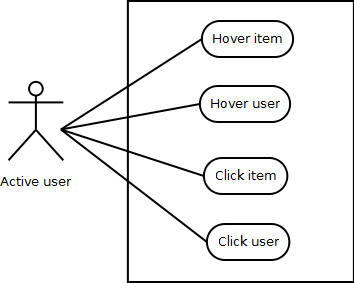
\includegraphics[scale=0.7]{img/usecase_diagram}
	\end{center}
  \caption{Use case diagram of the \emph{SoundSuggest} application.}
  \label{fig:use_case_diagram}
\end{figure}

%\FloatBarrier





% Resultaten en bespreking van het onderzoek.
\chapter{Iterative development}\label{chapter:prototype}

% Shirley et al. : human-centered design process
%This iterative process can be human-centered design process described in \cite{shirley:2009}.

This chapter describes how the idea presented in chapter \ref{chapter:literature_study} is tested and improved through different development cycles. First the evaluation and development techniques used for the tests are described.


\section{Methodology}\label{chapter:prototype:section:methodology}

\subsection{Prototyping}\label{chapter:prototype:section:methodology:subsection:development}

% rapid prototyping

There are three types of prototypes that were used in the iterations:

\begin{itemize}
	\item Paper prototype;
	\item Digital prototype with 'fake' data or interaction effects;
	\item Digital prototype with working implementation.
\end{itemize}

It is obvious that for each category the resources that are required to build the prototype differ. The objective is to filter out most of the issues in the low cost designs, avoiding a greater cost in the more expensive prototypes.

\emph{Paper prototyping}\index{paper prototyping} is defined as "a variation of usability testing where representative users perform realistic tasks by interacting with a paper version of the interface that is manipulated by a person 'playing computer', who doesn’t explain how the interface is intended to work"\cite{snyder:2003:web}. It is a technique for designing, testing, and refining user interfaces \cite{snyder:2003}, and is closely related to usability testing \cite{snyder:2003:web}. In the last decade it has become a regularly applied technique in major businesses such as IBM, Digital, Honeywell, and Microsoft among others\cite{snyder:2003}.

Digital prototypes capture a portion of the functionality in an application. In the early stages of the design process, this application usually works with static data, or a limited number of screen transitions. This allows for more flexibility when certain functionality has to be altered. In later iterations the static data is replaced with real data. In such prototypes, the effects of performance of algorithms and interface responsiveness can be analyzed in greater detail.


\subsection{Evaluation techniques}\label{chapter:prototype:section:methodology:subsection:evaluation}

The evaluation of an application prototype can be performed using one or more different techniques, and based on a range of varying criteria, such as: usability, usefulness, meaning, efficiency, accuracy and so on. Various techniques exist, such as questionnaires, usability engineering, expert evaluation, and usage tracking\cite{duval:2012:chi:evaluation}.

Methods may be \emph{formative}\index{formative!evaluation technique} or \emph{summative}\index{summative!evaluation technique}. Formative means that the evaluation occurs simultaneously with user task execution. Summative occurs after the user has performed all the required tasks\cite{duval:2012:chi:evaluation}.

The explanation system will be evaluated based on seven aims described by Tintarev and Masthoff \cite{tintarev:2007:SER:1547550.1547664} listed in table \ref{table:explanation:aims}. Also learnability and memorability, properties of usability as described by Nielsen\cite{nielsen:1993:UE:529793}, are also evaluated. An insight evaluation method developed by Chris North \cite{north:2006} is used to measure transparency, as described in section \ref{chapter:literature_study:section:user:subsection:insight}. Usability evaluation methods are used to measure satisfaction, efficiency, learnability and memorability. Trust, effectiveness, and persuasiveness are also evaluated during the user study. Scrutability is not supported by the explanation system.

Both usability and insight gaining methods are a variation on \emph{usability engineering}\index{usability engineering} called \emph{think aloud}\index{think aloud} user tests. Additionally, a type of questionnaires called \emph{system usability scale} (SUS)\index{system usability scale} \emph{questionnaires}\index{questionnaire} are used to obtain a quantification of the perceived usability by test users, in terms of perceived learnability and satisfaction. Such a quantification may allow us to identify positive or negative trends in the usability throughout the iterations.

In order to perform reliable usability tests, the test users have to be representative for the actual user population\cite{duval:2012:chi:evaluation, north:2006}. The tasks that are being used, have to be representative of the system usage. Tasks also have to correspond to research questions to obtain relevant results\cite{snyder:2003}.

The number of users can often be limited. As the number of detectable problems is likely to be finite, from a certain point on testing more users will not produce new or better results\cite{duval:2012:chi:evaluation, nielsen:2012:nngroup:diminishing_returns}. The graph in figure \ref{fig:nielsengraph}, adapted from \cite{nielsen:2012:nngroup:diminishing_returns}, illustrates this phenomenon.

Nielsen argues that as a rule of tumb, five test users is enough to acquire reliable and valuable test results. Instead of doing one test with 15 users, use three iterations with 5 users each. Based on the graph, the first iteration will discover the majority of the usability problems; the next two tests will uncover the remaining 15\% of issues. Of course, this only holds on the condition that tasks performed by the users are similar for each iteration. Between each iteration, corrections are applied to the design\cite{nielsen:2012:nngroup:diminishing_returns}. Between these groups of tests, detected usability problems are addressed, and hopefully resolved which can be verified in the next iteration.

\begin{figure}
	\begin{center}
		\includegraphics[width=250px]{img/nielsen2012_usertests}
	\end{center}
	\caption{The curve shows the user test's diminishing returns beyond a certain amount of test users; adapted from \cite{nielsen:2012:nngroup:diminishing_returns}.}
	\label{fig:nielsengraph}
\end{figure}


\subsubsection{Usability engineering}

In \cite{duval:2012:chi:evaluation}, two methods are described to perform usability engineering tests: usability labs, and think aloud\index{think aloud} testing. In a usability lab the user is observed while performing certain tasks. Data on task completion time, mouse clicks, eye-movement can be collected. Direct observation or cameras can be used to observe the user. To mimic real-life situations, also complete settings can be recreated in which the users would normally use the application\cite{duval:2012:chi:evaluation}.

Using usability labs can be rather costly, since labs need to be available and the required equipment may be expensive. The think aloud protocol is a variation on the usability lab method and is cheaper to perform, cf. 'discount usability engineering'\cite{duval:2012:chi:evaluation}. During a think aloud test, the user describes his/her reasoning for each action he/she undertakes\cite{nielsen:2012:nngroup:think_aloud}. This method has several advantages and disadvantages, as listed in table \ref{table:usability_engineering}, based on \cite{nielsen:2012:nngroup:think_aloud} and \cite{snyder:2003}.


\begin{table}%
	\begin{center}
		\begin{tabular}{l p{300px}}
			\hline
			Advantages		&		It is cheap to perform; \\
										&		It is robust; \\
										&		It is flexible; \\ % giving required freedom to perform insight tests
										&		It is convincing; \\
										&		It is easy to learn; \\
			\hline
			Disadvantages	&		It creates an unnatural situation, as users usually don't say out loud everything they are about to do or think; \\
										&		The user may tend to filter his/her statements to avoid saying things that he/she may find silly or uninteresting; \\
										&		The facilitator may introduce bias in user behavior if he/she provides too much information when answering or instructing users; \\
			\hline
		\end{tabular}
	\end{center}
	\caption{Advantages and disadvantages of the think aloud protocol.}
	\label{table:usability_engineering}
\end{table}

\subsubsection{Questionnaires}

To obtain information other than observational data, the user is presented with a summative questionnaire. Questionnaires are used to obtain subjective information from the user about the user's experiences. Table \ref{table:questionnaires} lists several advantages and disadvantages of the use of questionnaires in usability studies, based on \cite{kirakowski:2013}.

\begin{table}%
	\begin{center}
		\begin{tabular}{l p{300px}}
			\hline
			Advantages		&		Evaluates the point of view of the user; \\
										&		Measures gained from a questionnaire are to a large extent, independent of the system, users, or tasks to which the questionnaire was applied; \\
										&		Quick and cost effective; \\
			\hline
			Disadvantages	&		Only the user's reaction as the user perceives the situation; \\
										&		Lack of detail, as questionnaires are usually designed to fit a number of different situations; \\
										&		Subjective data must be enhanced with performance, mental effort, and effectiveness data. \\
			\hline
		\end{tabular}
	\end{center}
	\caption{Advantages and disadvantages of the questionnaires.}
	\label{table:questionnaires}
\end{table}


There are several standardized questionnaires. The one used for the application evaluation is the system usability scale\index{system usability scale} (SUS). A system usability scale test is a questionnaire that consists out of ten specific questions that attempts to measure the user's perception of the application's usability. Each question is answered by checking one out of five checkboxes: checkbox one corresponds to strong disagreement with the statement, the fifth checkbox corresponds to strong agreement with the statement\cite{sauro:2011}. The ten questions are listed in table \ref{table:sus_questions}.

To interpret SUS results, the scores should be compared on a percentile rank. Figure \ref{figure:sus_percentile} shows a graph by Jeff Sauro adapted from \cite{sauro:2011}. A SUS score of 80 means then that the perceived usability is higher than almost 90 percent of the products tested in Sauro's user studies.

\begin{figure}%
	\begin{center}
		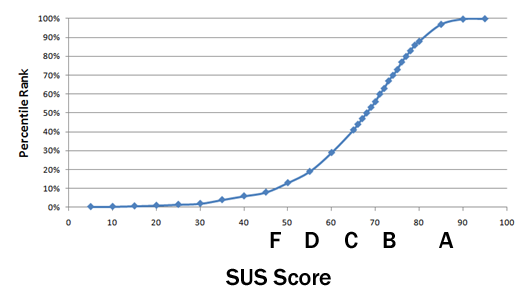
\includegraphics[width=280px]{img/sus_curve}%
	\end{center}
	% http://www.measuringusability.com/sus.php
	\caption{Percentile ranks associate with SUS scores and letter grades, adapted from \cite{sauro:2011}.}%
	\label{figure:sus_percentile}%
\end{figure}


\section{Iterations}

We will now give an overview of the setup for the user studies. In the next subsections we will discuss each iteration in more detail.

To increase domain relevance, it is important to have representative test users. The participants were selected from the campus and among acquaintances and were between $21$ and $27$ years of age. For all of the iterations combined, a total of $15$ users participated in the user study of whom $12$ were male and $3$ were female. Based on the categorization in table \ref{table:jennings:listeners}, $5$ users identied themselves as \emph{savants}, $7$ as \emph{enthousiasts}, and $3$ as \emph{casuals}. Although they had a notion of what a recommender system was, none of them knew how recommendation algorithms worked.

The test users were spread among four different iterations. Some of the users took part in multiple tests. The distribution of users can be seen in table \ref{table:evaluation:users}. There are two particular incentives to let users participate in more than one test:

\begin{enumerate}
	\item These users can provide direct feedback on changes made between the iterations that addressed certain usability issues.
	\item As insight builds up over time, it would be interesting to go beyond the scope of a single user test that only lasts $30$ to $60$ minutes. If given the opportunity, users may develop new ways to apply their previously obtained insights, amplifying its deep, serendipitous, complex and qualitative aspects.
\end{enumerate}

\begin{table}
	\caption{The distribution of test users used in the evaluations for each iteration.}
	\begin{center}
		\begin{tabular}{l | l l l l }
				\hline
																	& \multicolumn{4}{c}{\textbf{Iteration}} \\
																\cline{2-5}
																& $1$ & $2$ & $3$ & $4$ \\
			\hline
			Number of users						&	5 	&	5		&	5		&	10	\\
			From previous iterations	&	-  	&	2 	&	3		&	5	\\
			\hline
		\end{tabular}
	\end{center}
	\label{table:evaluation:users}
\end{table}

Over the four iterations the application was incrementally improved. Table \ref{table:iteration:aims} gives an overview of which aims were evaluated for the prototype in each iteration. The reason why trust, effectiveness, and persuasion are only tested in the last iteration, was that in iteration $1$ and $2$ no data from the active user was processed. As a result, it would be rather pointless to test for effectiveness if the user profile does not correspond to the active user's taste. In iteration three, we focus mainly on usability aspects.

\begin{table}
	\caption{The explanation aims that were evaluated in each iteration.}
	\begin{center}
		\begin{tabular}{l | l l l l }
			\hline
			\textbf{Aim} 							& \multicolumn{4}{c}{\textbf{Iteration}} \\
																\cline{2-5}
																& $1$ & $2$ & $3$ & $4$ \\
			\hline
			Tra. Sat., Efc., Learn.		&	x 	&	x		&	x		&	x	\\
			Mem.											&	  	&	x		&	x		&	x	\\
			Trust, Efk., Pers.				&	  	&	 		&	 		&	x	\\
			\hline
		\end{tabular}
	\end{center}
	\label{table:iteration:aims}
\end{table}



%%%%%%% ITERATION 1
\subsection{Iteration 1: paper prototype}\label{chapter:prototype:section:paper}

% 6. testen...
%		+ doel: wat wil je te weten komen?
%		+ methode: hoe ga je dat te weten komen?
%		+ rationale: welke andere manieren heb je overwogen en waarom niet weerhouden?
%		+ wie, wat, waar: n, demographics, logistics, ...
%		+ resultaten: wat heb je gemeten, geobserveerd? (zonder interpretatie)
%		+ besluit: wat ben je te weten gekomen? (link naar resultaten)
% 7. itereren...
%		+ doel: belangrijkste proble(e)m(en) dat/die je wil aanpakken
%		+ alternatieven: hoe kan je problemen aanpakken
%		+ keuze: en rationale
%		+ herneem die problemen bij volgende iteratie!

\subsubsection{The prototype}\label{chapter:prototype:section:paper:prototype}

The paper prototype that was tested, consisted out of a single screen. On this screen a visualization was drawn by hand. A number of copies were made of this drawing and by changing certain parts of the visualization, transitions within the visualization could be mimicked as users interacted with the screen. A selection of these screens are shown in figure \ref{figure:paper_prototype}.

% BEGIN FIGURE : paper prototype
\begin{figure}
	\centering
	\begin{subfigure}[t]{0.3\textwidth}
					\centering
					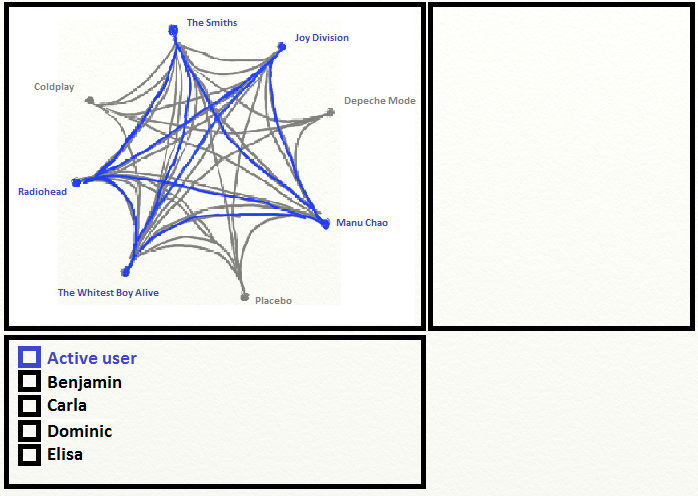
\includegraphics[width=\textwidth]{img/paper_prototype_default}
					\caption{The default visualization with the active users items highlighted.}
					\label{figure:paper_prototype_default}
	\end{subfigure}%
	~
	\begin{subfigure}[t]{0.3\textwidth}
					\centering
					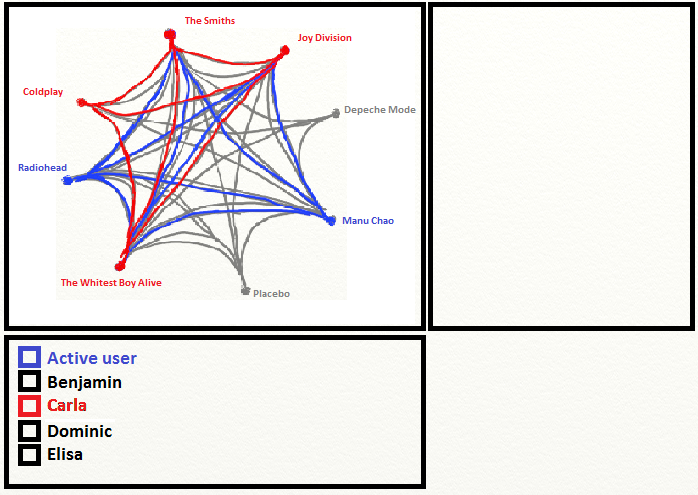
\includegraphics[width=\textwidth]{img/paper_prototype_user_click}
					\caption{Clicking/hovering a user list element.}
					\label{figure:paper_prototype_user_click}
	\end{subfigure}
	~
	\begin{subfigure}[t]{0.3\textwidth}
					\centering
					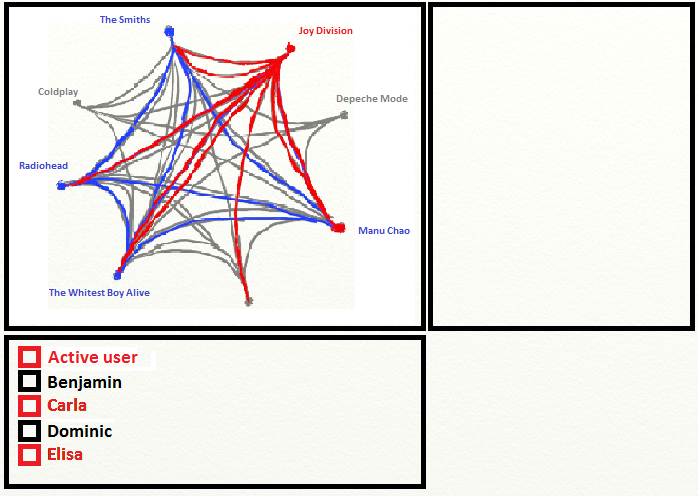
\includegraphics[width=\textwidth]{img/paper_prototype_item_click}
					\caption{Clicking/hovering an item node. When clicking a node, an additional screen would be shown next to the graph. On this screen artist information is displayed.}
					\label{figure:paper_prototype_item_click}
	\end{subfigure}
	\caption{A selection of the screens used in the user study with paper prototype.}%
	\label{figure:paper_prototype}%
\end{figure}

When a user would hover an artist or user name, the screen would be replaced with the corresponding new state of the screen. To ensure a certain degree of freedom, all possible screen states were drawn for the given graph. To keep this amount manageable within the scope of a relatively short user test, the number of artists was limited to eight, and the number of users to six, including the active user. Another reason for keeping graph size small, is that small graphs tend to be easier to interpret\cite{herman:2000}. In an environment where interactions aren't as smooth as in a real implementation, this may be of significance, keeping the principle of transparency\index{principle of transparency} in mind.


\subsubsection{Test parameters}\label{chapter:prototype:section:paper:setup}

Five test users between the ages of $22$ and $26$ were selected. Four of them identified as enthousiasts, one of them as a casual listener. Although they did not necessarily use recommendation systems to actively search for new music, they had a notion of what these systems were.

The focus of the test is on insight, i.e., transparency, and usability, covering satisfaction, learnability and efficiency:

\begin{enumerate}
	\item \textbf{Insight}: Verifying whether or not the user can gain insight into the recommendation rationale.
	\item \textbf{Usability}: Finding out the perceived usability of the application. Discovering usability issues through observation.
\end{enumerate}


%Each task is related to one of those objectives. ELABORATE
The list of tasks that were performed by the users is listed in appendix \ref{appendix:tasklists:prototype1}. The tasks description are based on a template\footnote{A \emph{PDF} version of this template can be found at: \url{http://www.paperprototyping.com/downloads/Ch6_task_template.pdf}} by Carolyn Snyder\cite{snyder:2003}.


\subsubsection{Test results}\label{chapter:prototype:section:paper:results}

% AVG, boxplots / question, boxplot overall

The average SUS score for this iteration was $77$. The distribution of results for each question is shown in figure \ref{fig:iterations_sus_scores_it1_boxplots}. The next paragraphs give a more in-depth analysis of the results.

\begin{figure}
	\begin{center}
		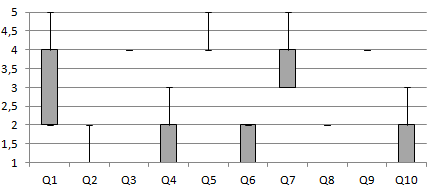
\includegraphics[width=8.3cm]{img/iterations_sus_scores_it1_boxplots}
	\end{center}
	\caption{The SUS results for each question for iteration 1.}
	\label{fig:iterations_sus_scores_it1_boxplots}
\end{figure}


\paragraph{Transparency}

The first part of the test was aimed at forming an initial mental model of the system without interacting with the visualization. When participants were asked to describe what they saw and try to explain the visualization, all of the participants identified the edges as certain relationship between artists. Most of them interpreted the relationship encoded in the edges as a content-based relationship; for example artists that have similar genres are connected.

Blue edges were usually correctly associated with the highlighted active user profile. This insight made one of the users see that the edges represent a co-occurance relationship, i.e., if a user has any set of two items in his/her profile, these items are connected.

If users became aware of the fact that blue nodes and edges corresponded to items that were already owned, item suggestions were easy to point out. In some cases this waited until the second step of the evaluation process where interaction was allowed.

The test users were asked what kind of interactions were possible with the visualization, and what the effects of these actions would be. All of the users listed left mouse clicks. Also dragging and scrolling were suggested by some participants. In that case participants were simply told that this kind of interaction was not supported. They expected to be able to manipulate the edge trajectory by dragging the edges were they wanted. However, clicking an edges is also not supported by the visualization. The effect of clicking a node was usually correctly predicted, although some users did not immediately see that related users would be highlighted as well.

In order to avoid restricting the user to predefined action patterns, the user was relatively free to explore the visualization in the second part of the test. Most participants started by clicking another user's icon and noted the resulting highlights in red in the graph. For one user the tasks in this step were a mere confirmation of the already established mental model. For most users this turned out to be an important moment in adjusting the first model. When alternating between clicking users icons, as well as between artist nodes and artist nodes and user icons the other users were able to correct their model in this step to finally form the correct picture of what the visualization was trying to convey. For two users this took significantly more time than for the other two remaining users.

The understanding of the relationship encoded in the edges, is key to grasping the whole idea behind the visualization. Once this was understood, all users could explain the recommender rationale. Moreover, users were able to point out an item recommendation that was more favourable than another suggestion, illustrating insight at a deeper level. For example using the total number of links to the active user profile, the total amount of related users, or a strong connection with a particular favourite item.


\paragraph{Satisfaction, learnability, and efficiency}

An average SUS score of $77$ suggests that the overal usability is considered to be good - also keeping in mind some of the limitations of paper prototypes. Still, some issues remain: the results for questions \texttt{Q1}, \texttt{Q4}, \texttt{Q7}, and \texttt{Q10} were the lowest. \texttt{Q1} is corresponds to the perceived usefulness, and is related to the overall satisfaction. Scores for \texttt{Q4}, \texttt{Q7}, and \texttt{Q10} may indicate that the learnability of the application can still improve.

Once users were able to develop a strategy for choosing recommendations, they could apply it rather easily in new cases. This suggests that if the user has passed initial learning phase, the system allows for efficient decision making.


\subsubsection{Conclusions}\label{chapter:prototype:section:paper:conclusion}


In conclusion, one user managed to get the complete mental model correct in the first step of the insight gaining process. The others were able to correct it in the second step. The model helped identifying a particular suggestion as more interesting than an others based on what they learned from the visualization.

Table \ref{table:iteration1:issues} gives an overview of the most important issues discovered in this iteration with their priority.

\begin{table}%
	\caption{Overview of the most important issues discovered in the first iteration, using the paper prototype.}
	\begin{center}
		\begin{tabular}{p{70px} | p{180px} | p{180px} }
			\hline
			\textbf{Problem} & \textbf{Priority} & \textbf{Solutions} \\
			\hline
			
			Learnability
			&
			\emph{Medium}: May be due to limitations of the paper prototype. Also, it is expected that a minimal effort is required to learn the system, instead of instantly understanding each aspect of the application.
			& (1) Providing more textual clues, as suggested by test users. (2) Moving towards a digital prototype with the user's actual library as data source. As the user has a better understanding of his/her own music library, it is likely that relationships within this data can be discovered more rapidly. % increased domain relevance
			\\
			
			Satisfaction
			&
			\emph{Medium}: Low value of usefulness may be due to the fact that the data is not personalized. The recommendations were also not based on an actual case, but were selected in the hope to appeal to the majority of test users.
			&
			(1) Again, moving towards real, personalized data may improve this aspect of the prototype.
			\\
			
			\hline
		\end{tabular}
	\end{center}
\label{table:iteration1:issues}
\end{table}

% In terms of the usability characteristics, the prototype ...

% terugkoppelen naar usability properties: learnability, Error rate and severity, Efficiency, Satisfaction, Memorability (see future user tests)
% does the explanation system provide transparency?
% can users gain insight into the visualization?




%%%%%%%% ITERATION 2
\subsection{Iteration 2: first digital prototype (SoundSuggest 1.x)}\label{chapter:prototype:section:soundsuggest1}

\subsubsection{The prototype}\label{chapter:prototype:section:soundsuggest1:prototype}

% changes from previous iteration
As the test users were able to discover the recommender rationale using the visualization, and no notable usability issues had arisen, we started working on the digital prototype. This prototype used static data, but already supported all the use cases listed in appendix \ref{appendix:use_cases}. The resulting prototype can be seen in figure \ref{figure:prototype_soundsuggest1}.


% iteration 2 : prototype
\begin{figure}
	\centering
	\begin{subfigure}[t]{0.3\textwidth}
					\centering
					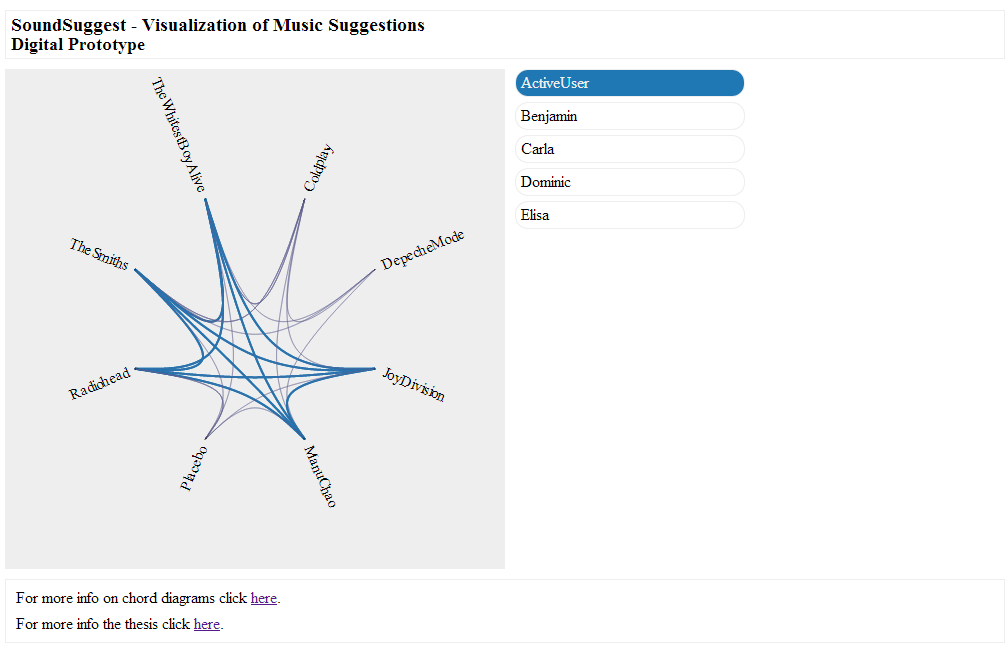
\includegraphics[width=\textwidth]{img/prototype_soundsuggest1_default}
					\caption{The default visualization with the active users items highlighted.}
					\label{figure:prototype_soundsuggest1_default}
	\end{subfigure}%
	~
	\begin{subfigure}[t]{0.3\textwidth}
					\centering
					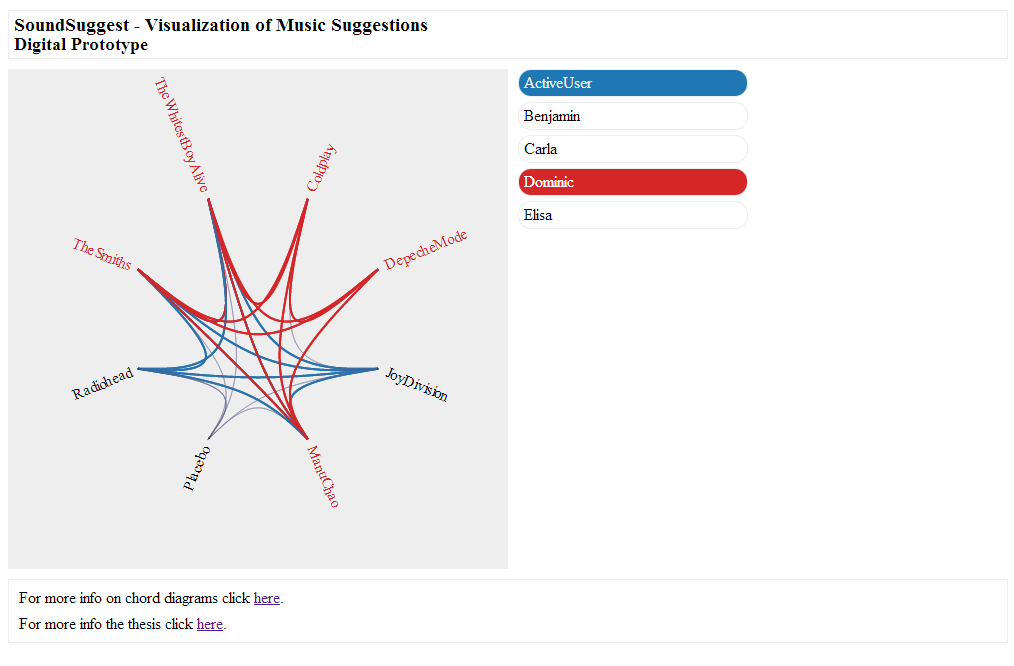
\includegraphics[width=\textwidth]{img/prototype_soundsuggest1_user_click}
					\caption{Clicking a user list element.}
					\label{figure:prototype_soundsuggest1_user_click}
	\end{subfigure}
	~
	\begin{subfigure}[t]{0.3\textwidth}
					\centering
					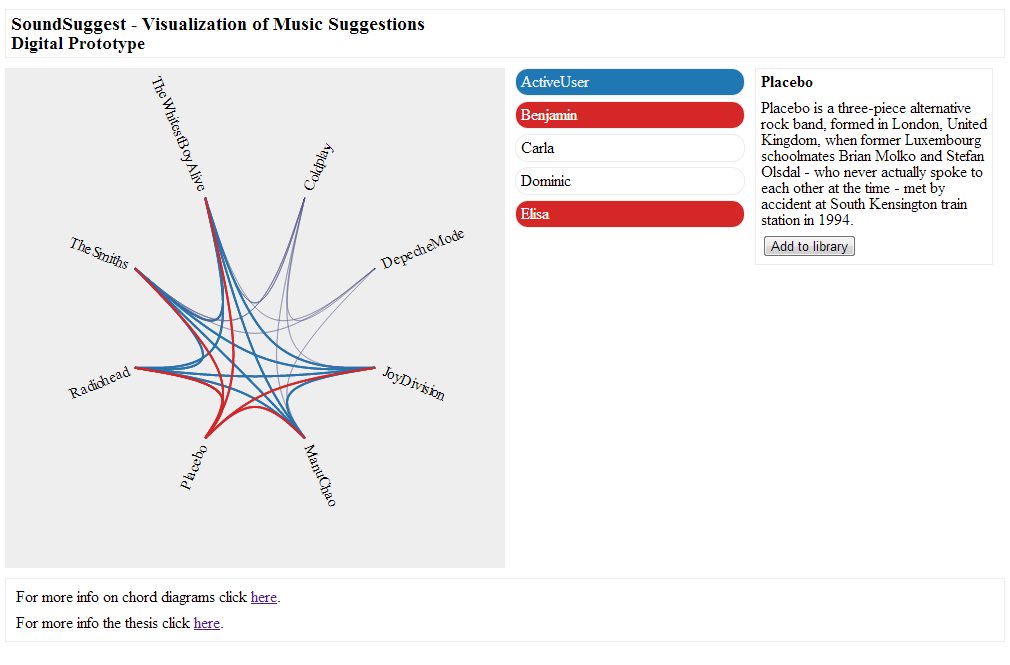
\includegraphics[width=\textwidth]{img/prototype_soundsuggest1_item_click}
					\caption{Clicking an item node.}
					\label{figure:prototype_soundsuggest1_item_click}
	\end{subfigure}
	\caption{A selection of the screens used in the user study with the first digital prototype.}%
	\label{figure:prototype_soundsuggest1}%
\end{figure}



\subsubsection{Test parameters}\label{chapter:prototype:section:soundsuggest1:setup}

Test users were selected in a similar manner as in the first iteration. Two test users from the previous iteration were tested again, the other three were new test users. The test users that had been tested before, were tested first. Memorability was evaluated for these subjects along with the other objectives for this iteration. Based on listening habits, one savant, two enthousiasts and two casual listeners were tested.

The objectives are the same as in iteration one. However, in addition to these objectives we want to find out how successful the transformation from paper to digital prototype had been. Also feedback was asked on a help file that was made for the application.

The tasks remained the same as in the previous iteration. The test users that were tested in the first iteration also were asked if there were any improvements or new issues going from the paper prototype to a digital one. Remarks made by these persons were also presented to the other test users.


\subsubsection{Test results}\label{chapter:prototype:section:soundsuggest1:results}

The average SUS score for this iteration was $79.5$. The distribution of results for each question is shown in figure \ref{fig:iterations_sus_scores_it2_boxplots}. A detailed analysis of the results is given in the following paragraphs.

\begin{figure}
	\begin{center}
		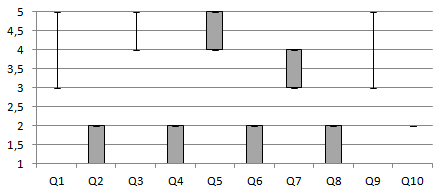
\includegraphics[width=8.3cm]{img/iterations_sus_scores_it2_boxplots}
	\end{center}
	\caption{The SUS results for each question for iteration 2.}
	\label{fig:iterations_sus_scores_it2_boxplots}
\end{figure}

\paragraph{Transparency}

Test users listed the list of neighbours, artist names. Most of them also noted that certain items and edges were coloured blue. One user also immediately saw that some of the other users and items did not have this colour and explained that these items corresponded to items recommended by these users. This participant further clarified that he expected that for each neighbour a similar coloured structure would exist as for the highlighted active user. When asked how this helped him understanding the recommendation rationale, the test user explained that these were users that had similar tastes as the active user. Items in these profiles were then candidate recommendations.

The other users did not find the recommendation rationale in the first step. When interacting with visualization however, they were able to tell similar stories. Again, the key to understanding the visualization turns out to be understanding what contextual information is that is encoded in the link between artist nodes. For most users this could be discovered by comparing the neighbour profile with the active user's profile on the graph.

With regard to the first iteration, one particular difficulty was mentioned by both users that tested the paper prototype: in the paper prototype parallel edges were easy to discern, but in the edge-bundling algorithm used, parallel edges will overlap in the resulting visualization. This makes it harder to see the connection between a clicked artist, and the number of neighbours that were highlighted. However, when the new test users were asked if they saw this as a problem, they acknowledged that this could help, but didn't see it as a major improvement. An improvement in the digital prototype was that the smoothness of interactions had of course greatly increased, which made it much easier to compare items and users, according to the test users.

% ---> no surprise that neighbour clicked --> insight, artist click ---> not so much

When asked to add one of the recommendations to the active user profile, all users could give one or more reasons, similar to the first iteration.


\paragraph{Satisfaction, learnability, memorability, and efficiency}

Some usability issues surfaced during the think aloud test. Two users thought that deselecting an item or user should be triggered by clicking somewhere outside the graph as well. Some test users complained that the help files did not have a table of contents or some sort of overview. Two users stated that it would be nice to have some kind of overview of the meaning behind each colour. Also having an extra colour to distinguish between selected profiles or edges and hover queries would be a welcome addition.

Overall, the SUS questionnaire results stayed more or less stable. Results for question \texttt{Q7} are still rather low, indicating that users still don't see the system as very easy to learn.

In terms of efficiency the same idea as in iteration $1$ applies. Of course, as interactions are much faster, this also has a positive effect on the efficiency of system usage.


\subsubsection{Conclusions}\label{chapter:prototype:section:soundsuggest1:conclusion}

% parallel edge occlusion: previously tested users say it would help, especially to see when two users share a parallel edge - otherwise hard to see which users have what items if overlap, but it is still clear.
% also, new test users were able to still get the recommender rationale

Overall, the transition from paper to digital prototype was successful, apart from the issue with parallel edges overlapping. Although it would be interesting if this problem could be solved, users indicated that was not a particular barrier for gaining insight into the recommendation rationale.

Different colours for hovering and selecting, although others thought this wasn't really necessary. Users suggested to add an option to choose between different encodings with an additional legend for the meaning of the different colours. Also options to alter the number of items shown were considered useful additions to the application's functionality.

Table \ref{table:iteration2:issues} gives an overview of the most important issues for iteration 2.

\begin{table}
	\caption{Overview of the most important issues discovered in the second iteration, using the first digital prototype.}
	\begin{center}
		\begin{tabular}{p{70px} | p{180px} | p{180px} }
			\hline
			\textbf{Problem} & \textbf{Priority} & \textbf{Solutions} \\
			\hline
			
			Parallel edges overlap
			&
			\emph{Low}: If possible, it would be nice to see this problem solved, but it is not considered to be a priority.
			&
			(1) Developing a new graph drawing algoritm, although this is perhaps beyond the scope of this thesis. (2) Allowing to change the bundling strength might improve the overall layout of the graph.
			\\
			
			Meaning behind colour encodings.
			&
			\emph{High}: As there already is a significant amount of implicit information in the visualization, it may be wise to give some direct clues as well.
			&
			(1) Show a legend of the visual encodings. (2) Enable the user to choose encodings him/herself. % see Ware: beware to not make this too complicated
			\\
			
			Deselecting an item
			&
			\emph{Medium}: Most users did not really had a problem with this, but it seems this could be solved easily enough.
			&
			(1) Adding a button to clear the current selection. (2) Track click events outside the visualization to clear the selection.
			\\
			
			\hline
		\end{tabular}
	\end{center}
\label{table:iteration2:issues}
\end{table}



%%%%%%% ITERATION 5
\subsection{Iteration 3: second digital prototype (SoundSuggest 2.x)}\label{chapter:prototype:section:soundsuggest2}

\subsubsection{The prototype}\label{chapter:prototype:section:soundsuggest2:prototype}

% changes from previous iteration
The layout from the previous iteration was retained, but this time the visualization was incorporated into a chrome suggestion that could be injected directly into the \emph{Last.fm} recommendations page, using real data.

An option menu was added with options to alter the data settings, and colour encodings. Data settings that could be altered were the number of recommendations shown, the number of top artists from the active user's profile shown, and the number of neighbours included in the visualization. Another option was to change the \emph{threshold}. The threshold corresponds to the clustering range of the data collection algorithm. A low threshold value will allow the user to have a link to a certain artist without owning it. Instead the user may own one or more related artists, i.e., the neighbour is required to have a link to an item inside a cluster of items, rather than a particular item. The settings menu is shown in figure \ref{figure:prototype_soundsuggest2_settings}.

\begin{figure}%
	\begin{center}
		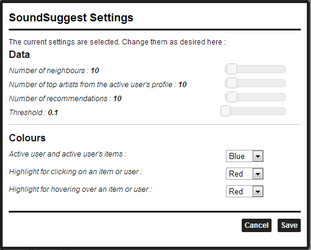
\includegraphics[width=200px]{img/prototype_soundsuggest2_settings}%
	\end{center}
	\caption{The settings menu of the second digital prototype.}%
	\label{figure:prototype_soundsuggest2_settings}%
\end{figure}


To solve the problem of deselecting an item, an additional button titled \emph{Clear selection}, was added in the menu bar. As the data loads, a spinner indicates to the user that the system is busy, as can be seen in figure \ref{figure:prototype_soundsuggest2_loading_data}. The resulting prototype is shown in figure \ref{figure:prototype_soundsuggest2}.

\begin{figure}%
	\begin{center}
		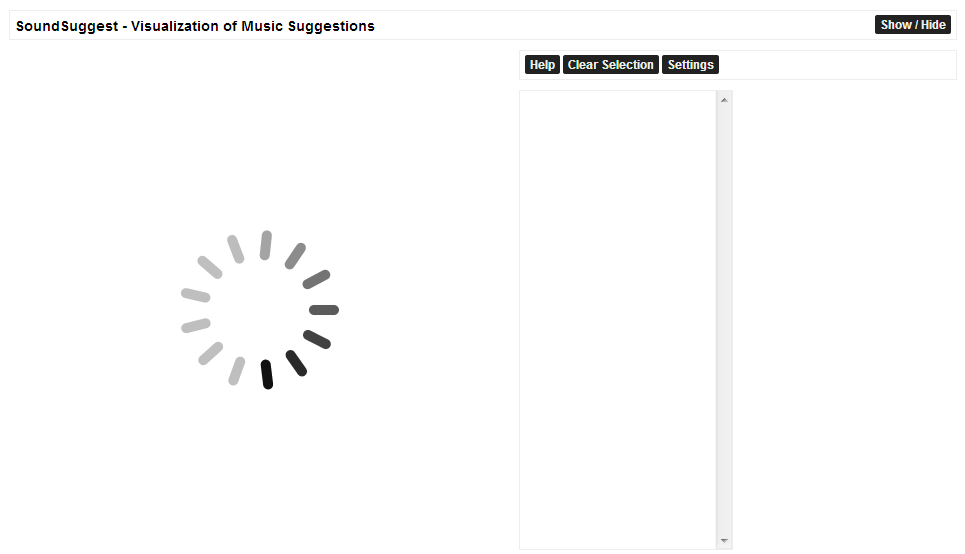
\includegraphics[width=200px]{img/prototype_soundsuggest2_loading_data}%
	\end{center}
	\caption{When the data is loading, a spinner is shown to indicate something is happening.}%
	\label{figure:prototype_soundsuggest2_loading_data}%
\end{figure}


% ITERATION 3
\begin{figure}
	\centering
	\begin{subfigure}[t]{0.3\textwidth}
					\centering
					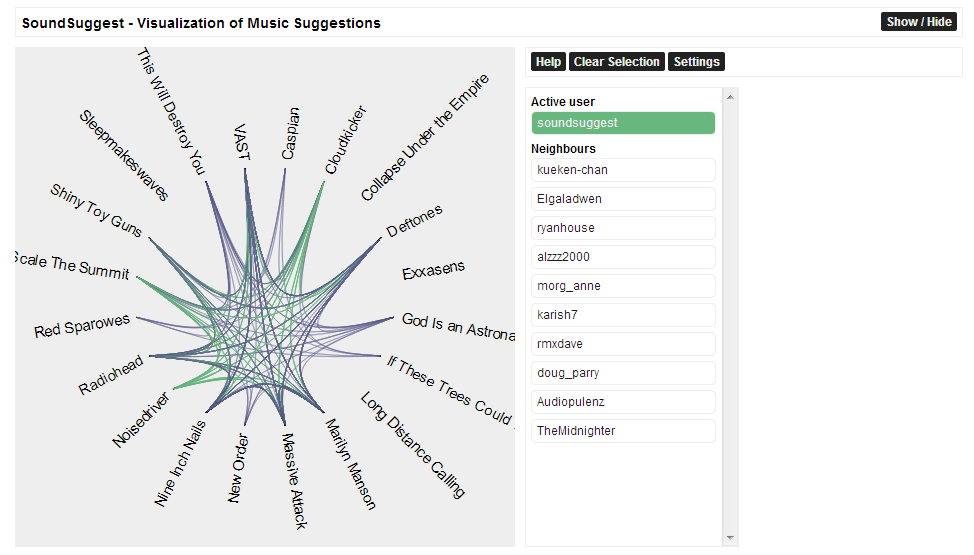
\includegraphics[width=\textwidth]{img/prototype_soundsuggest2_default}
					\caption{The default visualization with the active user's items highlighted.}
					\label{figure:prototype_soundsuggest2_default}
	\end{subfigure}%
	~
	\begin{subfigure}[t]{0.3\textwidth}
					\centering
					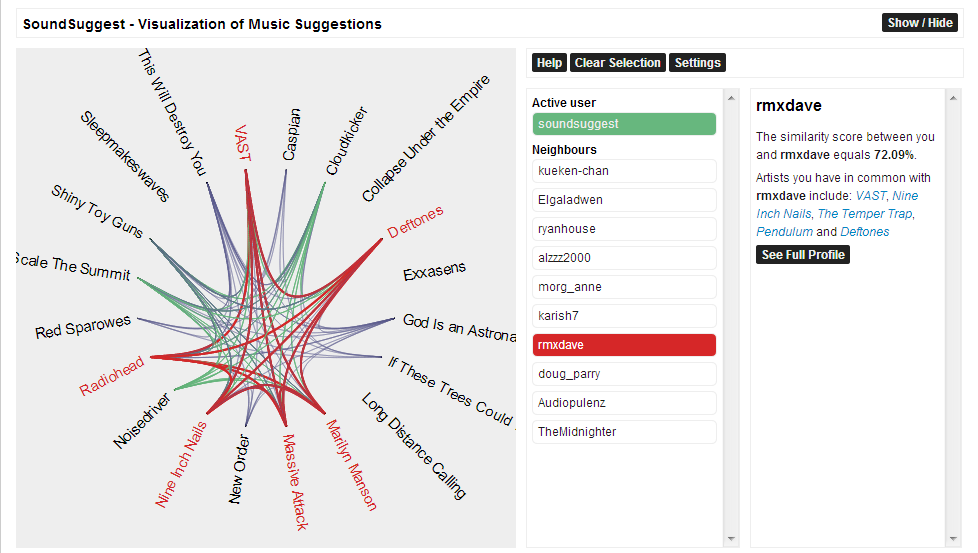
\includegraphics[width=\textwidth]{img/prototype_soundsuggest2_user_click}
					\caption{Clicking a user list element.}
					\label{figure:prototype_soundsuggest2_user_click}
	\end{subfigure}
	~
	\begin{subfigure}[t]{0.3\textwidth}
					\centering
					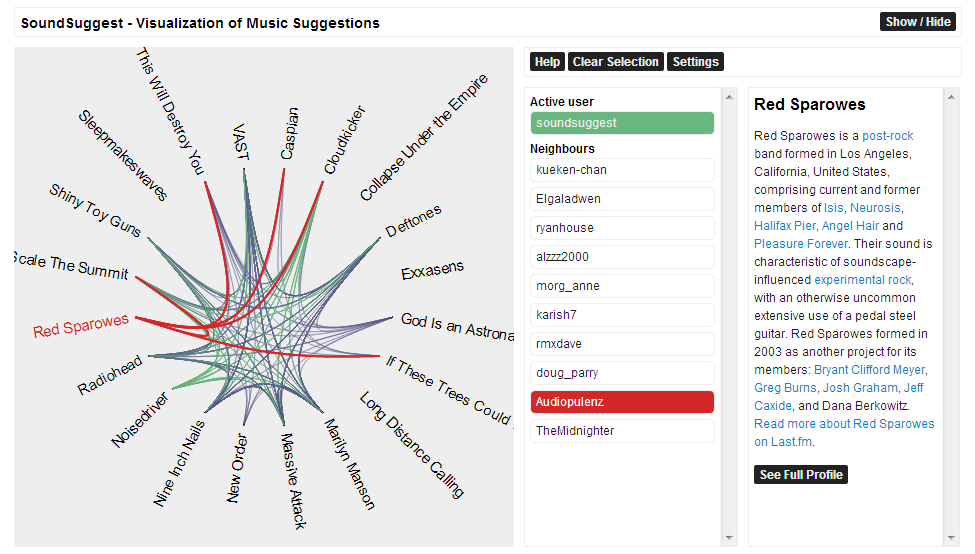
\includegraphics[width=\textwidth]{img/prototype_soundsuggest2_item_click}
					\caption{Clicking an item node.}
					\label{figure:prototype_soundsuggest2_item_click}
	\end{subfigure}
	\caption{A selection of the screens used in the user study with the third digital prototype.}%
	\label{figure:prototype_soundsuggest2}%
\end{figure}



\subsubsection{Test parameters}\label{chapter:prototype:section:soundsuggest2:setup}

Five test subjects were selected, who were \emph{Last.fm} users between the ages of $22$ and $26$. Three of them used the website or its \emph{Scrobbler} on a weekly basis or even more frequently, the other two only used \emph{Last.fm} on a monthly basis. Two users had tested both the paper and first digital prototype, one other user already had tested the paper prototype.

The objectives of the test remained the same. In addition to the previous objectives the performance of the application was investigated as well. Concerning usability, there were three areas of interest:

\begin{enumerate}
	\item \textbf{Visualization}: The general usability of the visualization according to new users.
	\item \textbf{Option menu}: General usability of the options menu.
	\item \textbf{Chrome extension}: The placement of the application into the \emph{Last.fm} recommendations page.
\end{enumerate}

The tasks listed in appendix \ref{appendix:tasklists:prototype2} were used to investigate these areas. Insight by new users could again be tested using the scheme in appendix \ref{appendix:tasklists:prototype1}. To get an idea of the learnablity and memorability of the application, test users from previous iterations were asked to explain the visualization rationale again before the rest of the test.


\subsubsection{Test results}\label{chapter:prototype:section:soundsuggest2:results}

The average SUS score for this iteration was $76.5$. The distribution of results for each question is shown in figure \ref{fig:iterations_sus_scores_it3_boxplots}.

\begin{figure}
	\begin{center}
		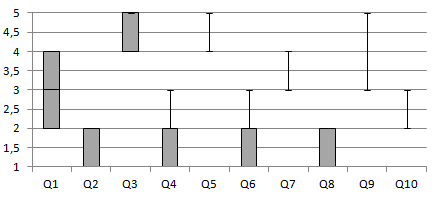
\includegraphics[width=8.3cm]{img/iterations_sus_scores_it3_boxplots}
	\end{center}
	\caption{The SUS results for each question for iteration 3.}
	\label{fig:iterations_sus_scores_it3_boxplots}
\end{figure}


\paragraph{Transparency and memorability}

Users from previous iterations were able to recall the visualization rationale from previous sessions, although two of them needed to interact with the visualization before they could remember it accurately. This suggests that the memorability of the explanation system is adequate. Based on previous experience and insight, one of these users explained he had found a new reasoning to select an artist based on the graph.

When testing insight for new users, no notable differences from previous iterations occurred. Theey also needed interaction with the visualization before the recommender rationale could be discovered.


\paragraph{Usability, satisfaction, efficiency, and learnability}

The settings menu was found by all users when asked to change the number of visualized items and/or users. One of the remarks when changing the data settings, was that the visualization would take long to load. As there were now more edges and nodes, some scalability issues came into play: some users complained that the increased number of edges would create clutter that made it hard to compare profiles.

Another issue that was mentioned was that it was hard to distinguish between recommendations once the test user started hovering over the listed neighbours. A test user from the previous session noted that this was less of a concern in the previous prototype, as the number of nodes was much lower.

The threshold option turned out to be very confusing, even with an explanation from the help files. Also, the results of changing the threshold were not visually pleasing either. As soon as the threshold would be over $0.1$, the connectivity dropped and some edges that were previously connected were no longer connected. This may also explain the fact that the average SUS score is lower than in previous iterations.

When adding a recommendation to the user profile, to see the changes in the profile, the whole page needed to be refreshed instead of just the visualization. Also, if the user would refresh or navigate away from the page, all of the data would have to be reloaded. This also has a negative effect on the satisfaction of system usage, which may also provide an additional explanation for the lower overal score.



\subsubsection{Conclusions}\label{chapter:prototype:section:soundsuggest2:conclusion}

Apart from the threshold option, the settings menu posed no notable difficulties. It would probably be better to use a default setting for the threshold, and remove the option from the settings menu altogether. The other options can remain as they are.

In conclusion, the main issues from the previous iteration have been solved. Table \ref{table:iteration3:issues} gives an overview of the most important issues for iteration $3$.

\begin{table}
	\caption{Overview of the most important issues discovered in the third iteration, using the second digital prototype.}
	\begin{center}
		\begin{tabular}{p{70px} | p{180px} | p{180px} }
			\hline
			\textbf{Problem} & \textbf{Priority} & \textbf{Solutions} \\
			\hline
			
			Threshold
			&
			\emph{High}: It is confusing and clearly has a negative impact on the overal user experience.
			&
			(1) Remove this functionality.
			\\
			
			Data load speed
			&
			\emph{High}: The main problem lies with the fact that changing the settings, reloading the page, and so on, results in reloading all the data, even though all the required data is known.
			&
			(1) Simply keeping a local copy of the latest version of the data. This version can then be updated either manually, or by checking for updates over a predefined time interval.
			\\
			
			Visual clutter
			&
			\emph{High}: Becomes an important problem as the graph size increases. May hinder the insight gaining process. May prohibit users from efficiently comparing user profiles and recommendations.
			&
			(1) Changing the graph layout: clustering nodes, changing edge-bundling strength, allowing to move nodes. (2) Change edge opacity to avoid visual clutter within dense regions of the graph. (3) Selectively hide elements temporary.
			\\
			
			\hline
		\end{tabular}
	\end{center}
\label{table:iteration3:issues}
\end{table}




%%%%%%% ITERATION 4
\subsection{Iteration 4: third digital prototype (SoundSuggest 3.x)}\label{chapter:prototype:section:soundsuggest3}

\subsubsection{The prototype}\label{chapter:prototype:section:soundsuggest3:prototype}

% changes from previous iteration

To reduce issues with distinguishability, an additional option was added to the settings menu to alter the \emph{tension} of the edges, i.e., the edge-bundling strength. This way, the user would be able to alter the layout to a certain extend.

To make it easier to distinguish between recommendations and top artists, the node labels for top artists are underlined in the graph.

A button to refresh the data and update the visualization was added to solve the problem of having to refresh the whole page to have the latest version of the data.

To avoid long waiting times when loading the page, the data that was loaded last was cashed. This way the latest data set could be loaded quickly from local storage. The refresh button can be used to get an up-to-date version of the data.

An example of the resulting visualization is shown in figure \ref{figure:prototype_soundsuggest3}.

% ITERATION 4
\begin{figure}
	\centering
	\begin{subfigure}[t]{0.3\textwidth}
					\centering
					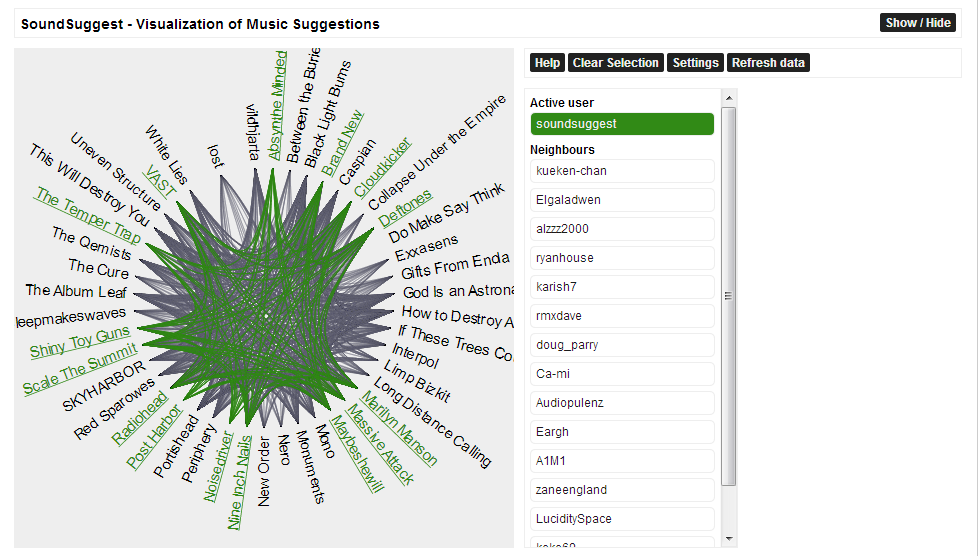
\includegraphics[width=\textwidth]{img/prototype_soundsuggest3_default}
					\caption{The default visualization with the active user's items highlighted.}
					\label{figure:prototype_soundsuggest3_default}
	\end{subfigure}%
	~
	\begin{subfigure}[t]{0.3\textwidth}
					\centering
					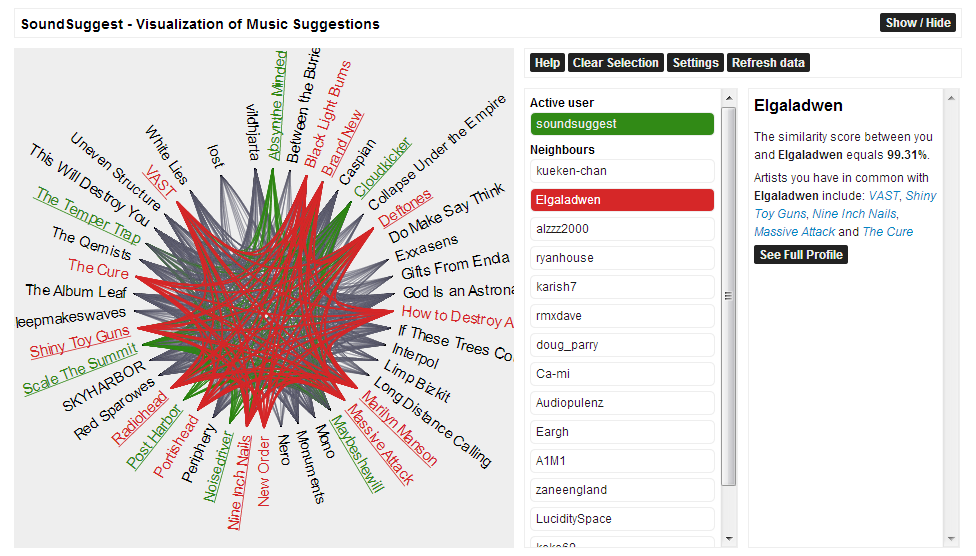
\includegraphics[width=\textwidth]{img/prototype_soundsuggest3_user_click}
					\caption{Clicking a user list element.}
					\label{figure:prototype_soundsuggest3_user_click}
	\end{subfigure}
	~
	\begin{subfigure}[t]{0.3\textwidth}
					\centering
					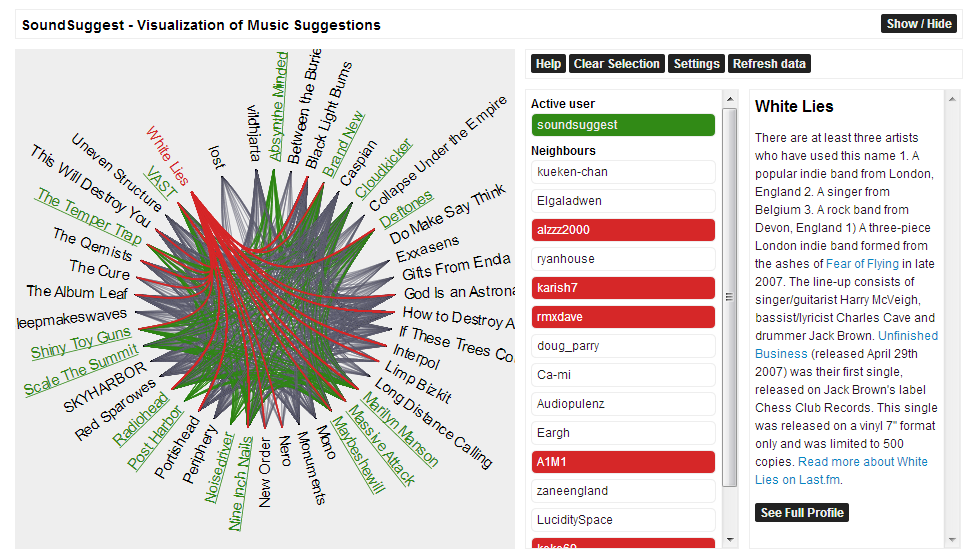
\includegraphics[width=\textwidth]{img/prototype_soundsuggest3_item_click}
					\caption{Clicking an item node.}
					\label{figure:prototype_soundsuggest3_item_click}
	\end{subfigure}
	\caption{A selection of the screens used in the user study with the third digital prototype.}%
	\label{figure:prototype_soundsuggest3}%
\end{figure}



\subsubsection{Test parameters}\label{chapter:prototype:section:soundsuggest3:setup}

Ten test users were selected. Three of these users already had experience with the application based on the previous iteration. Two of the other test users had tested one the first digital prototype. The other test users were new users. All of the test users had some experience with Last.fm or other music recommenders like \emph{Grooveshark}, \emph{Spotify} or \emph{Youtube}. If users didn't have a Last.fm account, they were asked to create one one to two weeks in advance and add their listening habits to their Last.fm profile.

% users: show diagrams with distribution for listening habits, Last.fm usage

For new users insight could again be tested using the tasks in appendix \ref{appendix:tasklists:prototype1}. The tasks listed in appendix \ref{appendix:tasklists:prototype3} were used to test the following explanation system properties: \emph{transparency}, \emph{effectiveness}, \emph{persuasion}, \emph{trust}, and \emph{satisfaction}.

Although \emph{scrutanability}\index{scrutanability} could have been tested by removing undesired recommendations from the list under the visualization, the visualization did not seem to include this information immediately when refreshing the data. It is also not really clear to what extend the information of removed suggestions is included into future recommendations by Last.fm's recommender algorithm.

% Efficiency is not explicitly tested here. For example benchmark tasks ... perceived effeiciency ...  rely on usability


\subsubsection{Test results}\label{chapter:prototype:section:soundsuggest3:results}

The average SUS score for this iteration was $80.5$. The distribution of results for each question is shown in figure \ref{fig:iterations_sus_scores_it4_boxplots}.

\begin{figure}
	\begin{center}
		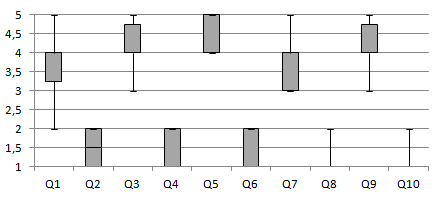
\includegraphics[width=8.3cm]{img/iterations_sus_scores_it4_boxplots}
	\end{center}
	\caption{The SUS results for each question for iteration 4.}
	\label{fig:iterations_sus_scores_it4_boxplots}
\end{figure}


\paragraph{Transparency}

All of the test users were able to describe the recommendation rationale. Most of them used a variation on the following: \textit{Last.fm looks for users that have a similar taste based on the active user's favourite artists, i.e., neighbours. Last.fm decides which items owned by these neighbours are interesting for recommendation based on preference by neighbours, i.e., top artists in the neighbouring profiles, and the total number neighbours that own these items}.


\paragraph{Trust, effectiveness, and persuasion}

Most users already knew more or less who the recommended artists were. For some users this would increase trust, as they basically forgot about them when building up listening history. For other users this would actually decrease their trust in the system as they simply were not interested in the recommendation. Interestingly \emph{Last.fm}'s own explanation for recommending the item was usually displeasing. \emph{Last.fm} would justify the recommendation by listing a number of 'similar' artists. Unfortunately, for some categories of artists there exists some bias in the recommendations. For example musicians that have a solo project and also played in a series of different bands lets Last.fm consider these artists as similar. Another example is that artist recommendations for bands and musicians that operate in a country with a less international music scene would be influenced by regional effects. Belgian bands would be considered similar just for beging Belgian to the point were all similar artist pages on the \emph{Last.fm} website would be Belgian regardless of their genre. Users confirmed that this kind of bias reduces the trust in the recommender system. On the other hand, it was interesting to see that this bias could actually be detected in the visualization as neighbours usually did not have edges going from items in their profile to these 'biased' recommendations.

When users did not know a certain recommendation, most users were interested if the recommendation occurred in one of the neighbouring profiles. In this sense the visualization helped persuade the users check out certain artists. From the six users that checked out an item they did not already know, four of them found at least one item that they liked and added to their profile. When discovering a new item that they liked, users admitted this significantly increased their trust in the recommender system, even more than when they found an item that they liked but already knew about.

Although the explanation system was not always as effective in helping to find good recommendations, it provided an additional means for the user to establish his/her own approach for finding recommendations. For example a user would look at neighbours for artist suggestions, rather than just the artist recommendations by \emph{Last.fm}.



\paragraph{Satisfaction, memorability, learnability, and efficiency}

The fact that the data set was cached made users much more confident in clicking links, as they didn't had to worry about long loading times.

A problem that remained was the scalability of the graph. When visualizing a total of over $40$ recommendations and top artists, loading times not only increase but the density caused by overlapping edges, makes it hard to compare user profiles. Although the tension parameter was visually pleasing, this did not completely resolve these scalability issues. Most users liked a tension in the area of $0.45$ to $0.60$ for graphs including up to $40$ nodes. Beyond this amount of nodes its effects became less important.

By underlining owned artists, it had become easier to compare user profiles. Users from previous iterations stated that this was definitively an improvement, but that there might still be better ways to visualize this. % still room for improvement

The distribution of scores for each separate SUS question for the last iteration is shown in figure \ref{fig:iterations_sus_scores_it4_boxplots}. The questions with the lowest scores were the first question and the seventh question. It should be noted thaht all test users were frequent \emph{Last.fm} users and also not all of the test users used the Chrome browser that was required for running the Chrome extension. Nonetheless there were test users that were very positive about the application in that respect as well. Although there were no negative votes for \texttt{Q7}, a lot of users were not convinced that using the application was easy to learn. There might still be some work left to make the application more accessible to casual users.




%The refresh button proved useful when adding a new recommendation.

% 1. Find three neighbours that are closely related to you, based on the visualization.
% 2. Find three recommended artists you think are interesting.
% 3. Explain the recommendation rationale (transparency).
% 4. Find a suggestion for an artist you didn't know about.
%		Would you like to check our this artist's profile and listen one or more songs by this artist (persuasion)?
%		Do you think the recommender system has made a good suggestion? Would you add it your profile (effectiveness)?
%		How does it affect your trust in the recommender system (trust)?





% risk pays of if the result is good!!


\subsubsection{Conclusions}\label{chapter:prototype:section:soundsuggest3:conclusion}

One issue that was resolved between the user tests was that the artist names that were used to create CSS \texttt{id} and \texttt{class} names sometimes contained special characters causing the visualization to not function correctly anymore. This was solved by using the hash value of the artist name instead. Although no new iteration was started for this alteration, this may have influenced some of the test results. Overall this only affected two participants.

Based from the choice of the tension parameter by users, a better default value for the tension setting would probably be around $0.55$.

%In future iterations the problems with overlapping edges should be addressed, for example by decreasing the alpha value of egdes that are not relevant to the selection. This is one of the clutter reduction techniques described in \cite{ellis:2007}.

%As trust increases 

Overall, the application scores well based on the user's feedback. It enables users to discover some characteristics of \emph{Last.fm}'s recommender.

Figure \ref{fig:iterations_sus_scores_boxplots} shows the evolution of the SUS values over the four iterations. Based on the percentile rank, the average score of $80.5$ for the final iteration produces a grade of \texttt{A}.

\begin{figure}
	\begin{center}
		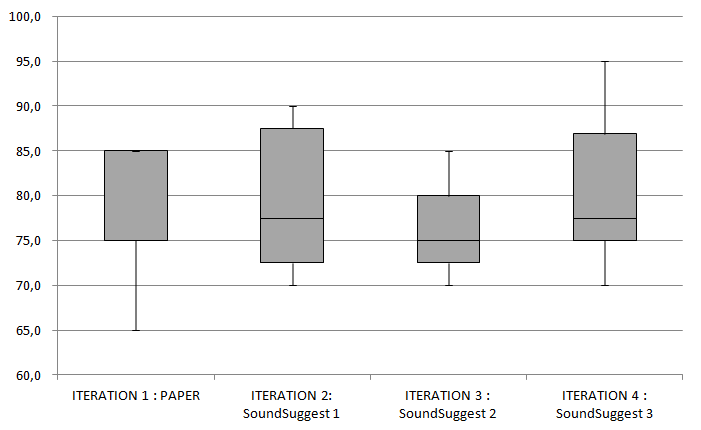
\includegraphics[width=8.3cm]{img/iterations_sus_scores_boxplots}
	\end{center}
	\caption{The evolution of the SUS values over the four iterations, visualized as box plots.}
	\label{fig:iterations_sus_scores_boxplots}
\end{figure}



Table \ref{table:iteration4:issues} gives an overview of the most important issues for iteration $4$.

\begin{table}
	\caption{Overview of the most important issues discovered in the fourth iteration, using the third digital prototype.}
	\begin{center}
		\begin{tabular}{p{70px} | p{180px} | p{180px} }
			\hline
			\textbf{Problem} & \textbf{Priority} & \textbf{Solutions} \\
			\hline
			
			Clutter reduction in dense graphs
			&
			\emph{High}: Visual clutter may hinder the insight gaining process, and may prohibit the user of comparing recommendations and user profiles effectively.
			&
			(1) Sorting the artists by recommendation or top artist would make it even easier to distinguish between owned and recommended artists. (2) Clutter reduction through change in opacity between elements that are relevant and irrelevant to the selection. (3) Selectively hiding users and their corresponding edges in the graph.
			\\
			
			Data load efficiency
			&
			\emph{Medium}: Some initial load of data will always be necessary, so for evaluation purposes this is probably a lesser concern.  To target a larger audience, this will become increasinly important.
			&
			(1) Using another algorithm that focuses less on node connectivity, but more on the quantity of data. When more items are involved, connectivity within the graph is likely to be higher as well. (2) Updating the graph as more data loads, depending on the predefined settings. (3) When refreshing the data, only update items that are new.
			\\
			
			Learnability
			&
			\emph{Medium}: Although the functionality of the application seems to be easy enough to learn, e.g. using the options in the settings menu, learning how the application can be useful, still takes up some time. This is probably reflected by lower scores for questions \texttt{Q1}, \texttt{Q7}, and \texttt{Q3}.
			&
			(1) Further refining labels and other visual clues for the end user.
			\\
			
			\hline
		\end{tabular}
	\end{center}
\label{table:iteration4:issues}
\end{table}

\chapter{Implementation: the SoundSuggest application}\label{chapter:implementation}

The application that was built for this thesis is called \emph{SoundSuggest}. It is a chrome extension that uses the D3 JavaScript library and the Last.fm API to inject the explanation system into the recommendations page of Last.fm\footnote{\url{http://www.last.fm/home/recs}}. In this chapter we will discuss the technologies we have used to create the application, the software design of the application and some specifics about the implementation of the application.


\section{Technologies}\label{chapter:implementation:section:technologies}

\subsection{Chrome extensions}\label{chapter:implementation:section:technologies:subsection:chrome}

Chrome Extensions are applications written in \emph{HTML}\index{HTML}, \emph{JavaScript}\index{JavaScript} and \emph{CSS}\index{CSS}\index{Cascading style sheet|see{CSS}}, that enhance the functionality of the Google Chrome web browser\cite{google:2012:extensions}.

There are different types of extensions. Browser actions are applications that can be launched regardless of the web page you are at. They appear as a button with a specified logo in the toolbar of the Chrome browser. By clicking the browser action you can specify to open up a tooltip or a popup\cite{google:2012:browseraction}. Page action extensions are meant to be shown when browsing specific web pages. They appear as an icon in the address bar. Page actions use content scripts to inject code into the web page\cite{google:2012:overview}.

The file \texttt{manifest.JSON} is one of the key areas of a chrome extension. It specifies the name and the version of your application as well as other important settings such as the type of the extension, scripts and security policies\cite{google:2012:manifest}.

Many extensions use a two-layered structure in which you have a background page and UI pages or content scripts\cite{google:2012:overview}. In the usual case the views are stateless and background pages are not. When the view needs some state, it requests the state from the background page. When the background page notices a state change, the background page tells the views to update\cite{google:2012:background}. Background pages can either be persistent or not. In the last case we are talking about so called event pages; they are opened and closed as needed\cite{google:2012:overview}.

There are various ways to use UI pages: you can open an HTML page in a popup, another tab or options page. The HTML pages inside an extension have complete access to each other's DOMs, and they can invoke functions on each other\cite{google:2012:overview}.

Content scripts are JavaScript scripts that are used to interact with a webpage opened in a browser tab. An important remark is that you should consider a content script part of the webpage it is injected into, rather than its parent extension. It can modify the DOM of the webpage but not the DOM of its background page. However it can ask its background page for data through listeners in the background page's script\cite{google:2012:overview}.



\subsection{The Last.fm API}\label{chapter:implementation:section:technologies:subsection:lastfm}

The \emph{Last.fm API}\index{Last.fm API}\index{Last.fm}\footnote{\url{http://www.last.fm/api}} offers great functionality such as the recommender system, Last.fm scrobbling and accessing and modifying your Last.fm profile information, aside from providing a large amount of data. To use the API, libraries have been developed for several technologies, such as \emph{JavaScript}\index{JavaScript}, \emph{PHP}, \emph{Python} and \emph{Actionscript} among others\cite{lastfm:2012:home}.

To build an application using the Last.fm API, you have to create an API account first at \url{http://www.last.fm/api/account/create}. Once you have been registered, you will receive an API key and an API secret.

For testing purposes it will also be handy to have a Last.fm account of your own. So if you haven't got one already sign up at their website. You might also want to one or more of their \emph{Scrobbler}\index{Scrobbler} applications. This will collect data from your music players to generate profile information that will be used to generate recommendations\cite{lastfm:2013:scrobbling}.

There are already several interesting applications that make use of the Last.fm API\index{Last.fm API}. Even more interesting perhaps is that some developers distribute free JavaScript libraries that act like a facade on the Last.fm API. The JavaScript library we will be using here, can be found on \emph{GitHub}\footnote{\url{https://github.com/fxb/javascript-last.fm-api}} and is written by \emph{Felix Bruns}.


\subsection{D3.js JavaScript Library}\label{chapter:implementation:section:technologies:subsection:d3js}

Visualizations for web applications can be built using \emph{scalable vector graphics}\index{scalable vector graphics} \emph{(SVG)\index{SVG|see{scalable vector graphics}}}. SVG is an XML-based language to describe two-dimensional graphics\cite{w3c:2011:svg}. It is supported by most of the latest versions of most popular browsers, including \emph{Chrome}, \emph{Firefox}, \emph{Internet Explorer 9}, \emph{Opera} and \emph{Safari}\cite{microsoft:2012:svg, w3c:2010:svg}.

\emph{D3.js}\index{D3.js} is a JavaScript library that uses the W3C standards \emph{HTML}, \emph{SVG} and \emph{CSS} to build data-driven documents\index{data-driven documents|see{D3.js}}\cite{bostock:2012:d3js}. There are various tutorials explaining the basics on how to use this library.

In short, to get started the library should be included in your web page. Next, using the D3 selectors, elements can be added and removed easily from the web page. The library also offers a number of built-in algorithms, as well as a series of example visualizations that can be customized as desired.


\subsection{Additional libraries}\label{chapter:implementation:section:technologies:subsection:libs}

In addition to the Last.fm API JavaScript library and D3.js, four other JavaScript libraries were used, namely:

\begin{itemize}
	\item \textbf{jQuery}\footnote{\url{http://jquery.com/}}\index{jQuery}: "jQuery is a fast, small, and feature-rich JavaScript library. It makes things like HTML document traversal and manipulation, event handling, animation, and Ajax much simpler with an easy-to-use API that works across a multitude of browsers"\cite{jquery:2013}.
	\item \textbf{jQuery UI}\footnote{\url{}}: "jQuery UI is a curated set of user interface interactions, effects, widgets, and themes built on top of the jQuery JavaScript Library"\cite{jqueryui:2013}.
	\item \textbf{Purl.js}\footnote{\url{https://github.com/allmarkedup/jQuery-URL-Parser}}: a library built on the jQuery library to retrieve GET parameters from the web page's URL.
	\item \textbf{Spinner.js}\footnote{\url{http://fgnass.github.io/spin.js/}}: a library that creates a spinner element with given parameters for customization.
\end{itemize}


\section{Software design and application architecture}\label{chapter:implementation:section:design}

The architecture of the application is shown in figure \ref{fig:architecture}. Five distict components can be identified that are of importance for the application:

\begin{itemize}
	\item \textbf{Last.fm recommendations page}: The HTML will we injected into this page. Although it is not a part of the source code, it poses certain limitations on the script. For example one should be careful not to override certain CSS definitions, and the injected code should fit into the page layout to achieve better looking results.
	\item \textbf{Content script}: The content script creates the injected HTML elements, handles user input, and delegates calls to the Last.fm API to the background script.
	\item \textbf{Background script}: the background script deals with local storage and calls to the Last.fm API.
	\item \textbf{Local storage}: The local storage of the Chrome browser can be used to store preferences.
	\item \textbf{Last.fm API}: The Last.fm API handles calls and returns the requested content.
\end{itemize}


\begin{figure}%
	\begin{center}
		\includegraphics[width=\columnwidth]{img/architecture}%
	\end{center}
	\caption{The architecture of the application.}%
	\label{fig:architecture}%
\end{figure}

Figures \ref{fig:sequence:part1} and \ref{fig:sequence:part2} show the sequence diagrams of what happens when loading the application. The first time the application is loaded, the user will have to authenticate the application. If the user does this, the content script will retrieve the token from the callback URL, and get a session key from the Last.fm API. This session key then stored. When the application is started again, the stored key can be retrieved from the local storage. Similarly other settings are loaded from local storage. If none have been stored so far, the default settings are returned and stored.

% Life lines :
%		ACTOR
%		(UI)
%		content script
%		background script
%		Local storage
%		Last.fm API

\begin{figure}%
	\begin{center}
		\includegraphics[width=\columnwidth]{img/seq_part1}%
	\end{center}
	\caption{Sequence diagram: opening the Last.fm recommendations page part 1: retrieving a session key.}%
	\label{fig:sequence:part1}%
\end{figure}

\begin{figure}%
	\begin{center}
		\includegraphics[width=\columnwidth]{img/seq_part2}%
	\end{center}
	\caption{Sequence diagram: opening the Last.fm recommendations page part 2: retrieving stored settings.}%
	\label{fig:sequence:part2}%
\end{figure}


Algorithm \ref{alg:loadingvis} shows how the data structure is constructed from calls to the Last.fm API\index{Last.fm API}. The resulting data structure is an approximation of the utility matrix on a local scale, i.e., the neighbourhood of the active user and the top artists of the active user. The time complexity of the algorithm depends on the number of artists $A$, i.e., the number of recommendations $R$ added to the number of top artists $T$, and the number of neighbours $N$ involved. The resulting time complexity is quadratic, i.e., $O(N^2)$, if $A$ approaches $N$.

%To be more precise, the effect of changing one of the data settings in the option menu on the data load is captured by the following formula $(R + T) * N$.


\begin{algorithm}[H]
		\SetAlgoLined
		\KwData{Active user $user$}
		\KwResult{Datastructure $D$}
		$D$ $\leftarrow$ $\emptyset$ \;
		$N$ $\leftarrow$ getNeighbours($user$)\;
		$U$ $\leftarrow$ union($user$, $N$)\;
		$T$ $\leftarrow$ getTopartists($user$)\;
		$R$ $\leftarrow$ getRecommendations($user$)\;
		$A$ $\leftarrow$ union($T$, $R$)\;
		% FOR EACH ARTIST
		\ForEach{artist $a$ in $A$}{
			% FOR EACH USER
			\ForEach{user $u$ in $U$}{
				$Similar$ $\leftarrow$ getSimilar($a$)\;
				$Score$ $\leftarrow$ compare(union($a$, $Similar$), $u$)\;
				% IF
				\If{$Score$ $>$ $threshold$}{
					$D$.$artistMAP$[$a$] $\leftarrow$ union($D$.$artistMAP$[$a$], $u$)\;
					$D$.$userMAP$[$u$] $\leftarrow$ union($D$.$userMAP$[$u$], $a$)\;
				}
			}
		}
	\caption{Loading the data for the visualization.}
	\label{alg:loadingvis}
\end{algorithm}


The corresponding sequence diagram is shown in figure \ref{fig:sequence:loadingvis}. The two calls within the inner loop have a large impact on the performance of the algorithm. Caching parts of the data structure is possible. However, small changes in the data may have an impact on the rest of data structure. For example if a user gets promoted to a neighbour and another gets demoted, it is impossible to know which user has to be removed from the data structure without comparing the lists of updated neighbours to the old version. Next the relevant neighbours should be removed from the data set and the new ones added. For artists that are promoted to the status of recommendation, there is a similar scenario. In this case, note that all of the users should be compared to the new items as well.


\begin{figure}%
	\begin{center}
		\includegraphics[width=\columnwidth]{img/seq_load_visualization}%
	\end{center}
	\caption{Sequence diagram: loading the visualization.}%
	\label{fig:sequence:loadingvis}%
\end{figure}



\section{Implementation}\label{chapter:implementation:section:implementation}

\subsection{Configuration file \texttt{manifest.JSON}}\label{chapter:implementation:section:implementation:subsection:configuration}

Aside from the basic parameters in the \texttt{manifest.JSON} file, such as \texttt{name}, \texttt{version}, \texttt{manifest\_version}, et cetera, there are several parameters that require some more attention. First of all, this extension is defined as a so-called page action. This is done by adding the page action with required attributes, namely certain icons and a default title, to the JSON file. The icon will become visible in the address bar when visiting a page defined in the \texttt{content\_scripts} parameter. In this case the script will become active when visiting the recommendations page of the \emph{Last.fm}\index{Last.fm} website. The various CSS and JavaScript used in the extension are also listed together with the content script.

As the application makes use of the storage functionality, the storage option should be added to the permissions. Since the application does calls to the Last.fm audioscrobbler, this link should be added to the permissions as well. Note that SSL is required when making external calls, otherwise the application won't even be accepted when uploading it to the chrome web store. The link should also be addded to the \texttt{content\_security\_policy} parameter of the manifest file.

To be able to access and load images, for example in the CSS definitions, it is necessary to add these to the \texttt{web\_accessible\_resources} parameter.

\subsection{The visualization \texttt{infovis}}\label{chapter:implementation:section:implementation:subsection:whitebox}

The visualization consists out of four main parts:

\begin{itemize}
	\item JSON data;
	\item JavaScript script;
	\item CSS style sheet;
	\item Custom implementation of certain methods.
\end{itemize}

\subsubsection{Data structure}

The JSON file structure is shown in listing \ref{listing:jsonfile}. It consists out of a list of artists and users that were retrieved using algorithm \ref{alg:loadingvis}. It can be generated by using the output of algorithm \ref{alg:loadingvis} as input for algorithm \ref{alg:createjson}. This is also a quadratic algorithm. However, its cost is much lower as it requires no expensive calls to the \emph{Last.fm API} in its inner loop.

\lstinputlisting[language=javascript, caption=The structure of the JSON file that is the input for the visualization script., label=listing:jsonfile]{src/datastructure.json}

%FOR EACH a IN dataArtists.keys
%	FOR EACH u IN artistData.get (a)
%		FOR d IN userData.get (u)
%			JSON.append ("edges", "item." + d.name + ".user." + u.name)
%		END-FOR
%	END-FOR
%	artist.put ("recommendation", u == active_user)
%	artist.put ("name", "item." + a.name)
%	JSON.append ("items", artist)
%END-FOR
%
%FOR EACH u IN userData.keys
%	user.put ("name", u.name)
%	user.put ("active", u == active_user)
%	FOR EACH a IN userData.get (u)
%		user.append ("owned", "item." + a.name)
%	END-FOR
%	JSON.append ("users", user)
%END-FOR

\begin{algorithm}[H]
	{
		\SetAlgoLined
		\KwData{Data structure $D$ from algorithm \ref{alg:loadingvis}, active user $active$.}
		\KwResult{JSON file $JSON$ as in listing \ref{listing:jsonfile}.}
		$JSON$ $\leftarrow$ $\{\}$ \;
		% artistMAP = map where artists are keys, for each key there is a list of users.
		% FOR EACH ARTIST
		\ForEach{Artist $a$ in $D$.$artistMap$.$keys$}{
			$artist$ $\leftarrow$ $\{\}$ \;
			$artist$.put ("name", "item." + $a$.$name$)\;
			$isrecommendation$ $\leftarrow$ false \;
			% FOR EACH USER
			\ForEach{User $u$ in $D$.$artistMap$[$a$]}{
				% userMAP = map where users are keys, for each key there is a list of artists.
				\If{$u$.equals ($active$)}{
					$isrecommendation$ $=$ true\;
				}
				\ForEach{Artist $d$ in $D$.$userMap$[$u$]}{
					$artist$.append ("edges", "item." + $d$.$name$ + ".user." + $u$.$name$)\;
				}
			}
			$artist$.put ("recommendation", $isrecommendation$)\;
			$JSON$.append ($artist$)\;
		}
		\ForEach{User $u$ in $D$.$userMap$.$keys$}{
				% FOR EACH USER
				$user$ $\leftarrow$ $\{\}$ \;
				$user$.put ("name", $u$.$name$)\;
				$user$.put ("active", $u$.equals ($active$))\;
				% userMAP = map where users are keys, for each key there is a list of artists.
				\ForEach{Artist $d$ in $D$.$userMap$[$u$]}{
					$user$.append ("owned", "item." + $d$.$name$)
				}
				$JSON$.append ($user$)\;
			}
		}
	\caption{Loading the data for the visualization.}
	\label{alg:createjson}
\end{algorithm}


\subsubsection{The visualization script}

Once the data structure has been constructed, it is plugged into the script. Listing \ref{listing:createwhitebox} shows how this is done in \emph{JavaScript}, assuming that the variables $LAYOUT$ and $DATA$ are known. The script uses the data to generate nodes, edges in an \texttt{SVG} element, and a list of users as \texttt{LI} elements in an \texttt{UL} element next to the visualization.

For this visualization, a \emph{D3.js} hierarchical edge-bundling example by Michael Bostock\cite{bostock:2012:edgebundling} was adapted. The major changes to the original code are the extension of the original data structure as explained in the previous section, and the addition of extra CSS classes to support interactions with the user list, which are discussed in the next section. In conclusion, for a detailed description of the visualization code, we refer to the D3.js website\footnote{The original code of the hierarchical edge-bundling example can be found at \url{http://bl.ocks.org/mbostock/1044242}.}.


\lstinputlisting[language=javascript, caption=Create a new Whitebox object for given settings and data., label=listing:createwhitebox]{src/create_whitebox.js}

\subsubsection{Style sheet}

To support hover and click interactions, each node and each user \texttt{LI} element has an \emph{onmouseover}, \emph{onmouseout}, and \emph{click} event listener attached to it. When one of these events is triggered, the appropriate classes are added or removed from these elements. Table \ref{table:interactions} shows which classes are activated for which interaction. Each of these classes in also combined with another set of classes as listed in table \ref{table:colours}. By changing the colour classes for nodes, edges and \texttt{LI}'s, colour patterns chosen by the end user are applied on the fly.


\begin{table}%
	\begin{center}
		\begin{tabular}{l | l l}
			\hline
			\textbf{Interaction}		& \texttt{SVG} Node in \textbf{\#chart svg} & User \texttt{LI} in \textbf{ul\#users }
			\\
			\hline
			Click node		& \textit{.link-item-clicked} & \textit{.user-item-clicked} \\
										& \textit{.node-item-clicked} & \\
			Click user		& \textit{.user-clicked} 			& \textit{.user-clicked} \\
										& \textit{.link-user-clicked} & \\
										& \textit{.node-user-clicked} & \\
			Hover node		& \textit{.node-item-mouseover} 	& \textit{.user-item-mouseover} \\
										& \textit{.user-item-mouseover}		& \\
			Hover user		& \textit{.node-user-mouseover} 	& \textit{.user.user-mouseover} \\
										& \textit{.link-user-mouseover}		& \\
			\hline
		\end{tabular}
	\end{center}
	\caption{Overview of the classes that added for each supported interaction for each interaction target.}
	\label{table:interactions}
\end{table}


\begin{table}%
	\begin{center}
		\begin{tabular}{l | l l l}
			\hline
			& \textbf{Blue}		& \textbf{Green} & \textbf{Red}
			\\
			\hline
			Active user &	\textit{.blue-active}	& \textit{.green-active} & \textit{.red-active} \\
			Mouseover 	&	\textit{.blue-mouseover}	& \textit{.green-mouseover} & \textit{.red-mouseover} \\
			Click				&	\textit{.blue-clicked}	& \textit{.green-clicked} & \textit{.red-clicked} \\
			\hline
		\end{tabular}
	\end{center}
	\caption{Overview of the classes that added for each supported colour.}
	\label{table:colours}
\end{table}





% Een conclusie, waarin een globale discussie van de onderzoeksresultaten wordt opgenomen. Eventueel kunnen hierin suggesties gedaan worden voor toekomstig onderzoek.
\chapter{Conclusion and future work}\label{chapter:conclusion}

% CONTENTS :
% Geef een overzicht van het door jou geleverde werk. Zorg dat het duidelijk is wat je eigen inbreng is en wat je elders gevonden hebt.
% Vergelijk de oorspronkelijke doelstelling met wat je bereikt hebt.
% Vermeld de belangrijkste problemen die je had bij het verwezenlijken van die doelstellingen.
% Wees kritisch en geef de voor- en nadelen van jouw oplossing en vergelijk je bekomen resultaat met beschikbare alternatieven.
% Geef aan welke uitbreidingen en verfijningen je nog zou kunnen/willen doen als je er de tijd voor had.
% 	FUTURE WORK
% 		visualization of content-based recommendation:
%			distance functions of feature vectors in a spatial map
%				...
% 		using this thesis as a starting point with visualization, sensemaking, etc. in literature study
%			using the whitebox in another context than music recommendation

In the literature we discussed recommender systems, the general context for recommender systems. We also listed general properties of recommender systems, described three recommendation approaches, and listed typical issues and shortcomings of recommender systems. One of these issues is the black box problem for which the end user fails to gain insight into the recommendation process and as a result may have little trust in its recommendations. To solve this problem an explanation system can be used that explains the recommendation rationale.

In the next part of the litature study we looked at various ways to visualize this rationale. We came up with a graph-based visualization representing the underlying utility matrix of collabrative recommendation, that uses Holten's edge-bundling algorithm along with node reduction to reduce the number of data dimensions, inspired by a visualization by Valdis Krebs.

Subsequently we looked at an evaluation method for visualization insight by Chris North. We also investigated the insight gaining process established by Klein et al. Finally we adapted Ware and Mitchell's visual thinking algorithm to describe how a user would interact with the visualization to solve a certain problem.

A number of visual explanation systems were discussed and we used a number of criteria by Tintarev and Masthoff to compare them.

Chapter \ref{chapter:requirements} investigated the target users, possbile scenarios of use and more elementary scenarios captured in use cases.

In chapter \ref{chapter:prototype} we looked at the different design and evaluation methods. The second part of this chapter described four different iterations in which a total of 15 test users observed while testing and evaluating the application. Between each iteration the detected usability issues were addressed and tested in the next. all the test users gained insight into the recommendation process and were able explain the recommendation rationale.

The objective that was could not be reached was to enable users to actively steer the recommendation process. This is due to the fact that the Last.fm API did not support this functionality. Of course an alternative could have been to make use of other methods in the API to construct our own custom recommender system, but we have chosen to explain the artist recommendations made by the actual Last.fm recommender instead. Another possibility could have been to use another recommender system altogether, but from the systems that were investigated, no significant additional functionality was discovered that could have overcome these issues.

Future work may include addressing problems with visual clutter, and slow data load. Also, the visual explanation system could be tested using other data sets and collaborative recommendation systems. Another possibility is to increase the interaction possibilities. For example by allowing interaction with edges the user could dig deeper into the relationship between artists and the corresponding users.








% ------------------------- Bibliography --------------------------
% 
% -----------------------------------------------------------------
%% A small distance to the other stuff in the table of contents (toc)
\addtocontents{toc}{\protect\vspace*{\baselineskip}}

%% The Bibliography
%% ----------------
%% ==> You need a file 'literature.bib' for this.
%% ==> You need to run BibTeX for this (Project | Properties... | Uses BibTeX)
\addcontentsline{toc}{chapter}{References} %'Bibliography' into toc
%\nocite{*} %Even non-cited BibTeX-Entries will be shown.
%\bibliographystyle{alpha} %Style of Bibliography: plain / apalike / amsalpha / ...
\bibliographystyle{abbrv}
\bibliography{bib/references}


%% Index
%% -----
%\clearpage
%\addcontentsline{toc}{chapter}{Index}
%\printindex

%% Appendices
%% ----------
\clearpage
\addcontentsline{toc}{chapter}{Appendices}
% Appendices: Hierin worden de delen van het onderzoek opgenomen die essentieel zijn voor het werk, maar die de leesbaarheid van de tekst zouden verlagen bv. door de lengte (wiskundige afleidingen, experimentele data, voorbeelden, figuren, etc.).
\appendix


\chapter{Use cases}\label{appendix:use_cases}

%%%%%%%%%%%%%%%USE CASE 1
\begin{table}[h]
\caption{Use case 1 \textit{Hover item}}
\begin{center}
	\begin{tabular}{ l p{300px} } % l = left-aligned column; p{...px} = paragraph with specified width.
		\hline
		\textbf{Primary actor:}	& Active user \\
		\textbf{Preconditions:}	& The application has access to the active user's profile; \\
														& The visualization has successfully loaded; \\
		\textbf{Basic flow:}	& (1) The user enters the area of an item node in the graph; \\
													& (2) The system highlights the nodes and edges that are directly connected to the target node (popout technique); \\
													& (3) The system highlights icons next to the graph corresponding to neighbours that have the target item in their profile; \\
													& (4) The user exits the node area; \\
													& (5) The system shows the default layout of the graph; \\
		\hline
	\end{tabular}
\end{center}
\label{tab:use_case1}
\end{table}



%%%%%%%%%%%%%%%USE CASE 2
\begin{table}[h]
\caption{Use case 2 \textit{Hover neighbour}}
\begin{center}
	\begin{tabular}{ l p{300px} }
		\hline
		\textbf{Primary actor:}	& Active user \\
		\textbf{Preconditions:}	& The application has access to the active user's profile; \\
														& The visualization has successfully loaded; \\
		\textbf{Basic flow:}	& (1) The user enters the area of a neighbour icon next to the graph; \\
													& (2) The system highlights the neighbour's icon; \\
													& (3) The system highlights the nodes and edges that connect items that are in the profile of the selected user; \\
													& (4) The user exits the icon area; \\
													& (5) The system shows the default layout of the graph; \\
		\hline
	\end{tabular}
\end{center}
\label{tab:use_case2}
\end{table}



%%%%%%%%%%%%%%%USE CASE 3
\begin{table}[h]
\caption{Use case 3 \textit{Click item}}
\begin{center}
	\begin{tabular}{ l p{300px} }
		\hline
		\textbf{Primary actor:}	& Active user \\
		
		\textbf{Preconditions:}	& The application has access to the active user's profile; \\
														& The visualization has successfully loaded; \\
		
		\textbf{Basic flow:}	& (1) The user clicks an item node in the graph; \\
													& (2) The system highlights the nodes and edges that are directly connected to the target node; \\
													& (3) The system highlights icons next to the graph corresponding to neighbours that have the target item in their profile; \\
													& (5) The system displays additional information about the item and options in an area next to the visualization; information includes a brief introductory text and top tracks; options include the possibility to add the item to the active user's profile. \\
		
		\textbf{Alternate flow:}	& (2.a) the item was already selected: the item is now deselected; \\
		
		\hline
	\end{tabular}
\end{center}
\label{tab:use_case3}
\end{table}


%%%%%%%%%%%%%%%USE CASE 4
\begin{table}[h]
\caption{Use case 4 \textit{Click neighbour}}
\begin{center}
	\begin{tabular}{ l p{300px} }
		\hline
		\textbf{Primary actor:}	& Active user \\
		
		\textbf{Preconditions:}	& The application has access to the active user's profile; \\
														& The visualization has successfully loaded; \\
		
		\textbf{Basic flow:}	& (1) The user clicks an item node in the graph; \\
													& (2) The system highlights the nodes and edges that are directly connected to the target node; \\
													& (3) The system highlights icons next to the graph corresponding to neighbours that have the target item in their profile; \\
													& (4) The system displays additional information about the item and options in an area next to the visualization; information includes a brief introductory text and top tracks; options include the possibility to add the item to the active user's profile. \\
		
		\textbf{Alternate flow:}	& (2.a) the neighbour was already selected: the neighbour is now deselected; \\
		
		\hline
	\end{tabular}
\end{center}
\label{tab:use_case4}
\end{table}


% Questions for the user tests for each iteration
\chapter{Task lists for the user tests}\label{appendix:tasklists}

\section{Task list 1: testing insight and usability}\label{appendix:tasklists:prototype1}

The user is given some context, i.e., the user knows he/she is using a recommender system to find new music and he/she has a number artists in his/her artist library.

\begin{table}
	\caption{Task 1.1: hypothesis generation, no interaction allowed.}
	\begin{tabular}{ p{80px} | p{350px} }
		\hline
		\textbf{Goal/Output}			& Getting an idea of the user's mental model about the visualization when he/she is not allowed to interact with it. \\
		\textbf{Inputs}						& The user has an account, and has built up some listening history. \\
		\textbf{Assumptions}			& The user is logged in. The data has loaded. \\
		\textbf{Steps}						& The user will try to get an overview of the displayed data. Through eye-movements he/she will explore the visualization. The user forms a hypothesis on the visualization rationale. \\
		\textbf{Estimated time} 	& $5$ to $10$ minutes. \\
		\textbf{Instructions}			&
		
		Answer the following questions without interacting with the visualization:
		\begin{enumerate}
			\item Describe what you see. Which visual elements stand out? Which general structures can be identified?
			\item What do you think the visualization does?
			\item Which the elements of the user interface, do you think allow interaction?
			\item What do you think will happen when you:
				\begin{itemize}
					\item hover over an node of the graph?
					\item hover over one of the users?
					\item click on an item?
					\item click on a user?
				\end{itemize}
		\end{enumerate}
		\\
		\hline
	\end{tabular}
	\label{table:task:t1}
\end{table}

\begin{table}
	\caption{Task 1.2: Further familiarization, interaction allowed.}
	\begin{tabular}{ p{80px} | p{350px} }
		\hline
		\textbf{Goal/Output}			& Getting an idea of the user's mental model about the visualization. \\
		\textbf{Inputs}						& See table \ref{table:task:t1}. \\
		\textbf{Assumptions}			& See table \ref{table:task:t1}. \\
		\textbf{Steps}						& The user verifies his/her initial mental model through interactions with the visualization. If the initial mental model is not confirmed, it is adjusted. \\
		\textbf{Estimated time} 	& \\
		\textbf{Instructions}			&
		Try to interact with the visualization. Answer the following questions:
		\begin{enumerate}
			\item Which of the artists displayed in the graph are artist suggestions?
			\item What are the links or edges in the visualization?
			\item	Suppose you want to add an item to your profile, what steps would you undertake?
		\end{enumerate}
		\\
		\hline
	\end{tabular}
	\label{table:task:t2}
\end{table}


\begin{table}
	\caption{Task 1.3: Adding an artist to the music library and motivating the choice(s) made.}
	\begin{tabular}{ p{80px} | p{350px} }
		\hline
		\textbf{Goal/Output}			& \\
		\textbf{Inputs}						& \\
		\textbf{Assumptions}			& \\
		\textbf{Steps}						& \\
		\textbf{Estimated time} 	& \\
		\textbf{Instructions}			&
		Add an item to your profile. Answer the following questions:
		\begin{enumerate}
			\item Why did you choose that particular item?
			\item Can you give any other reasons why you should pick this item?
			\item Can you give reasons for choosing one of the other items?
		\end{enumerate}
		\\
		\hline
	\end{tabular}
	\label{table:task:t3}
\end{table}



\section{Task list 2: testing the first version of the settings menu}\label{appendix:tasklists:prototype2}

Tables \ref{table:task:t4}, \ref{table:task:t5}, and \ref{table:task:t6} give an overview of the tasks used in the user study to evaluate the settings menu.

\begin{table}
	\caption{Task 2.1: Change the number of shown recommendations up to $20$.}
	\begin{tabular}{ p{80px} | p{350px} }
		\hline
		\textbf{Goal/Output}			& The number of displayed recommendations in the graph has changed. \\
		\textbf{Inputs}						& \\
		\textbf{Assumptions}			& \\
		\textbf{Steps}						& \\
		\textbf{Estimated time} 	& \\
		\textbf{Instructions}			& \\
		\hline
	\end{tabular}
	\label{table:task:t4}
\end{table}


\begin{table}
	\caption{Task 2.2: Change the threshold to $0.3$.}
	\begin{tabular}{ p{80px} | p{350px} }
		\hline
		\textbf{Goal/Output}			& \\
		\textbf{Inputs}						& \\
		\textbf{Assumptions}			& \\
		\textbf{Steps}						& \\
		\textbf{Estimated time} 	& \\
		\textbf{Instructions}			& \\
		\hline
	\end{tabular}
	\label{table:task:t5}
\end{table}



\begin{table}
	\caption{Task 2.3: Change the colours to an encoding that you like.}
	\begin{tabular}{ p{80px} | p{350px} }
		\hline
		\textbf{Goal/Output}			& \\
		\textbf{Inputs}						& \\
		\textbf{Assumptions}			& \\
		\textbf{Steps}						& \\
		\textbf{Estimated time} 	& \\
		\textbf{Instructions}			& \\
		\hline
	\end{tabular}
	\label{table:task:t6}
\end{table}







\section{Task list 3: testing the performance of the evaluation system}\label{appendix:tasklists:prototype3}


\begin{table}
	\caption{Task 3.1: Find three neighbours that are closely related to you, based on the visualization.}
	\begin{tabular}{ p{80px} | p{350px} }
		\hline
		\textbf{Goal/Output}			& The user can find three closely related neighbours and can give an adequate motivation for his/her choice. \\
		\textbf{Inputs}						& \\
		\textbf{Assumptions}			& \\
		\textbf{Steps}						& \\
		\textbf{Estimated time} 	& \\
		\textbf{Instructions}			&
		Find three neighbours that are closely related to you, based on the visualization. Explain why these are closer neighbours than others neighbours on the graph.
		\\
		\hline
	\end{tabular}
	\label{table:task:t7}
\end{table}


\begin{table}
	\caption{Task 3.2: Find three recommended artists you think are interesting.}
	\begin{tabular}{ p{80px} | p{350px} }
		\hline
		\textbf{Goal/Output}			& The user can find three interesting artist recommendations and give an adequate motivation for his/her choice. \\
		\textbf{Inputs}						& \\
		\textbf{Assumptions}			& \\
		\textbf{Steps}						& \\
		\textbf{Estimated time} 	& \\
		\textbf{Instructions}			&
		Find three recommended artists you think are interesting. Explain why these artists are more interesting than other recommendations shown in the graph.
		\\
		\hline
	\end{tabular}
	\label{table:task:t8}
\end{table}


\begin{table}
	\caption{Task 3.3: Explain the recommendation rationale (transparency).}
	\begin{tabular}{ p{80px} | p{350px} }
		\hline
		\textbf{Goal/Output}			& \\
		\textbf{Inputs}						& \\
		\textbf{Assumptions}			& \\
		\textbf{Steps}						& \\
		\textbf{Estimated time} 	& \\
		\textbf{Instructions}			&
		Explain the recommendation rationale. How do you think Last.fm's recommender system works?
		\\
		\hline
	\end{tabular}
	\label{table:task:t9}
\end{table}


\begin{table}
	\caption{Task 3.4: Find a suggestion for an artist you didn't know about.}
	\begin{tabular}{ p{80px} | p{350px} }
		\hline
		\textbf{Goal/Output}			& \\
		\textbf{Inputs}						& \\
		\textbf{Assumptions}			& \\
		\textbf{Steps}						& \\
		\textbf{Estimated time} 	& \\
		\textbf{Instructions}			&
		Find a suggestion for an artist you didn't know about.
		\begin{itemize}
			\item Would you like to check our this artist's profile and listen one or more songs by this artist (persuasion)?
			\item Do you think the recommender system has made a good suggestion? Would you add it your profile (effectiveness)?
			\item How does it affect your trust in the recommender system (trust)?
		\end{itemize}
		\\
		\hline
	\end{tabular}
	\label{table:task:t10}
\end{table}




% The statistics of the social media usage
\chapter{Quantified self}\label{appendix:statistics}


Figure \ref{fig:toggl:stats} and table \ref{table:toggl:stats} give an overview of the activities for thsis thesis based on \emph{Toggl}\footnote{\url{https://www.toggl.com/}} entries. Table \ref{table:socialmedia:stats} shows the statistics for social interactions related to the thesis, including tweets using the \#thesis12 hash tag on \emph{Twitter}\footnote{\url{https://www.twitter.com/}}, posts on the \emph{SoundSuggest} blog\footnote{\url{http://soundsuggest.wordpress.com/}} and comments on blogs by peers, and read papers and suggestions on \emph{Tinyarm}\footnote{\url{http://atinyarm.appspot.com/}}.


%%%%%%%%%%%%%%%%%%%%%%%%%%%%%%%%TOGGL STATS 1
\begin{figure}
	
	\begin{center}
	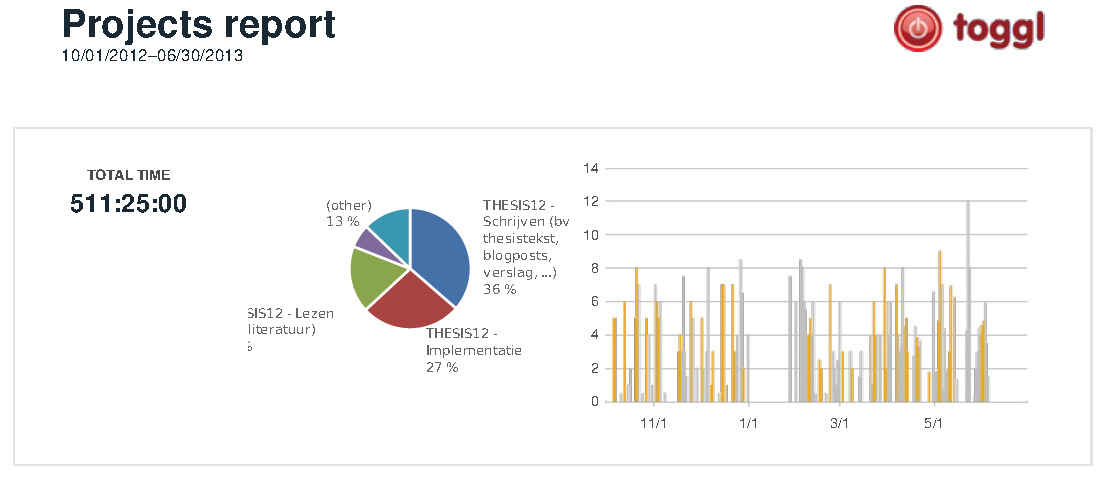
\includegraphics[width=\columnwidth]{img/toggl_graphs}%
	\end{center}
	
	\caption{Graphs generated by \emph{Toggl}.}
	\label{fig:toggl:stats}
\end{figure}



%%%%%%%%%%%%%%%%%%%%%%%%%%%%%%%%TOGGL STATS 2
\begin{table}%

	\caption{Approximation of the distribution of activities for this thesis, based on \emph{Toggl} entries.}
	
	\begin{center}
		\begin{tabular}{ p{350px} | r }
			\hline
			\textbf{Activity} & \textbf{Time} \\
			\hline
			Schrijven (bv. thesistekst, blogposts, verslag, ...) 																								& 186:00:00 \\
			Implementation 																																											& 136:50:00 \\
			Lezen (bv. literatuur) 																																							& 91:10:00 \\
			Evaluatie 																																													& 31:50:00 \\
			Presentatie (bv. voorbereiding, geven) 																															& 17:00:00 \\
			Reflectie (bv opstellen planning, interpretatie resultaten, etc.) 																	& 13:30:00 \\
			Ontwerp 																																														& 12:30:00 \\
			Social Network Actvities (bv.twitter, comments op andere blogs, suggesting papers met tinyarm, etc) & 11:20:00 \\
			Meetings (bv. met begeleider, mede-studenten, etc.) 																								& 11:15:00 \\
			\hline
			\hline
			Total time 																																													& 511:25:00 \\
			\hline
		\end{tabular}
	\end{center}
	\label{table:toggl:stats}
\end{table}


%%%%%%%%%%%%%%%%%%%%%%%%%%%%%%%%SOCIAL MEDIA STATS
\begin{table}%

	\caption{The social interactions related to the project.}
	
	\begin{center}
		\begin{tabular}{ l | l | r }
			\hline
			\textbf{Tool} 		& \textbf{Unit} 						& \textbf{Quantity} \\
			\hline
			\emph{Twitter} 		& Tweets \emph{\#thesis12}	& $\pm66$		\\
			\emph{Wordpress}	& Posts 										& $36$		\\
												& Pages 										& $15$		\\
												& Comments 									& $\pm30$	\\
			\emph{Tinyarm}		& Papers (read)							&	$45$		\\
												& Recommended								&	$3$			\\
			\hline
		\end{tabular}
	\end{center}
	\label{table:socialmedia:stats}
\end{table}




\chapter{Scientific article}
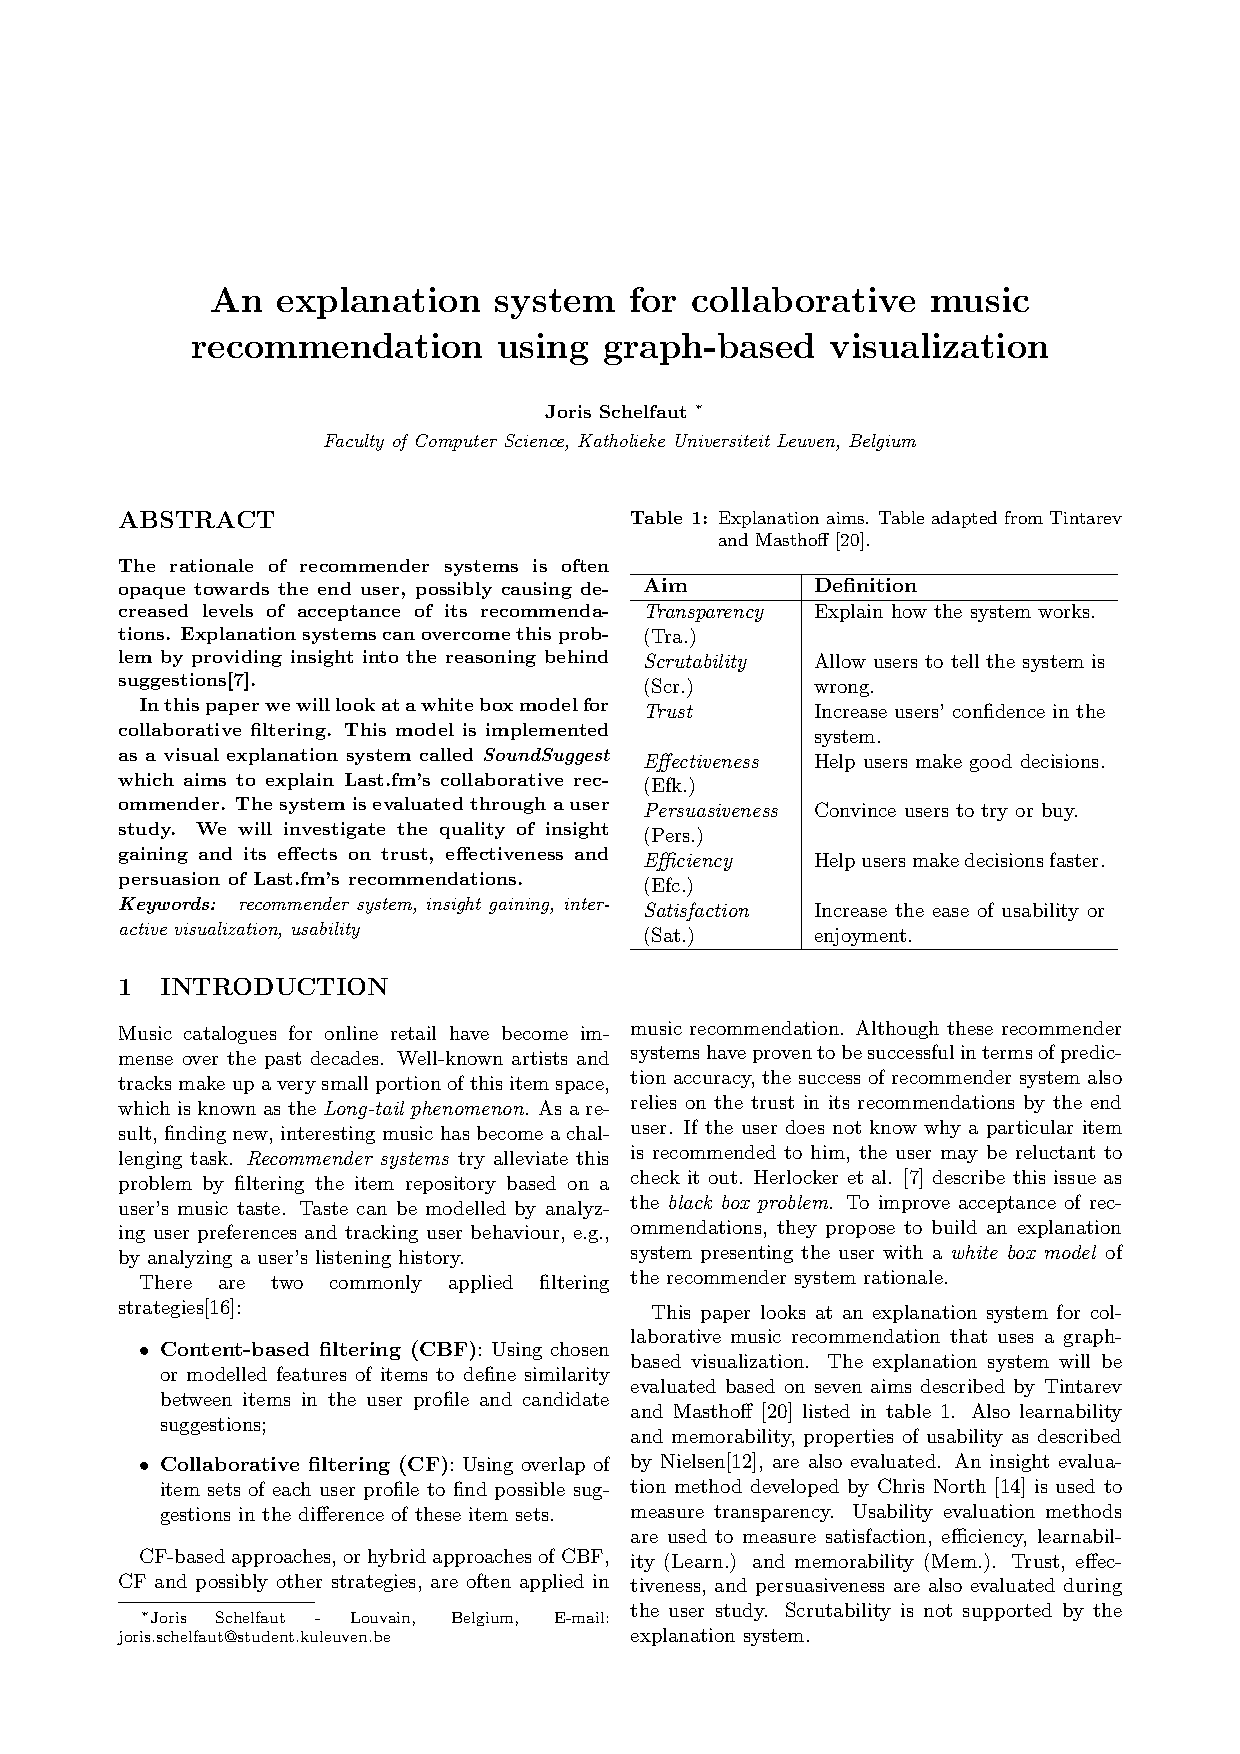
\includepdf[pages={1-9}]{pdf/scientific_article}

\chapter{Poster}
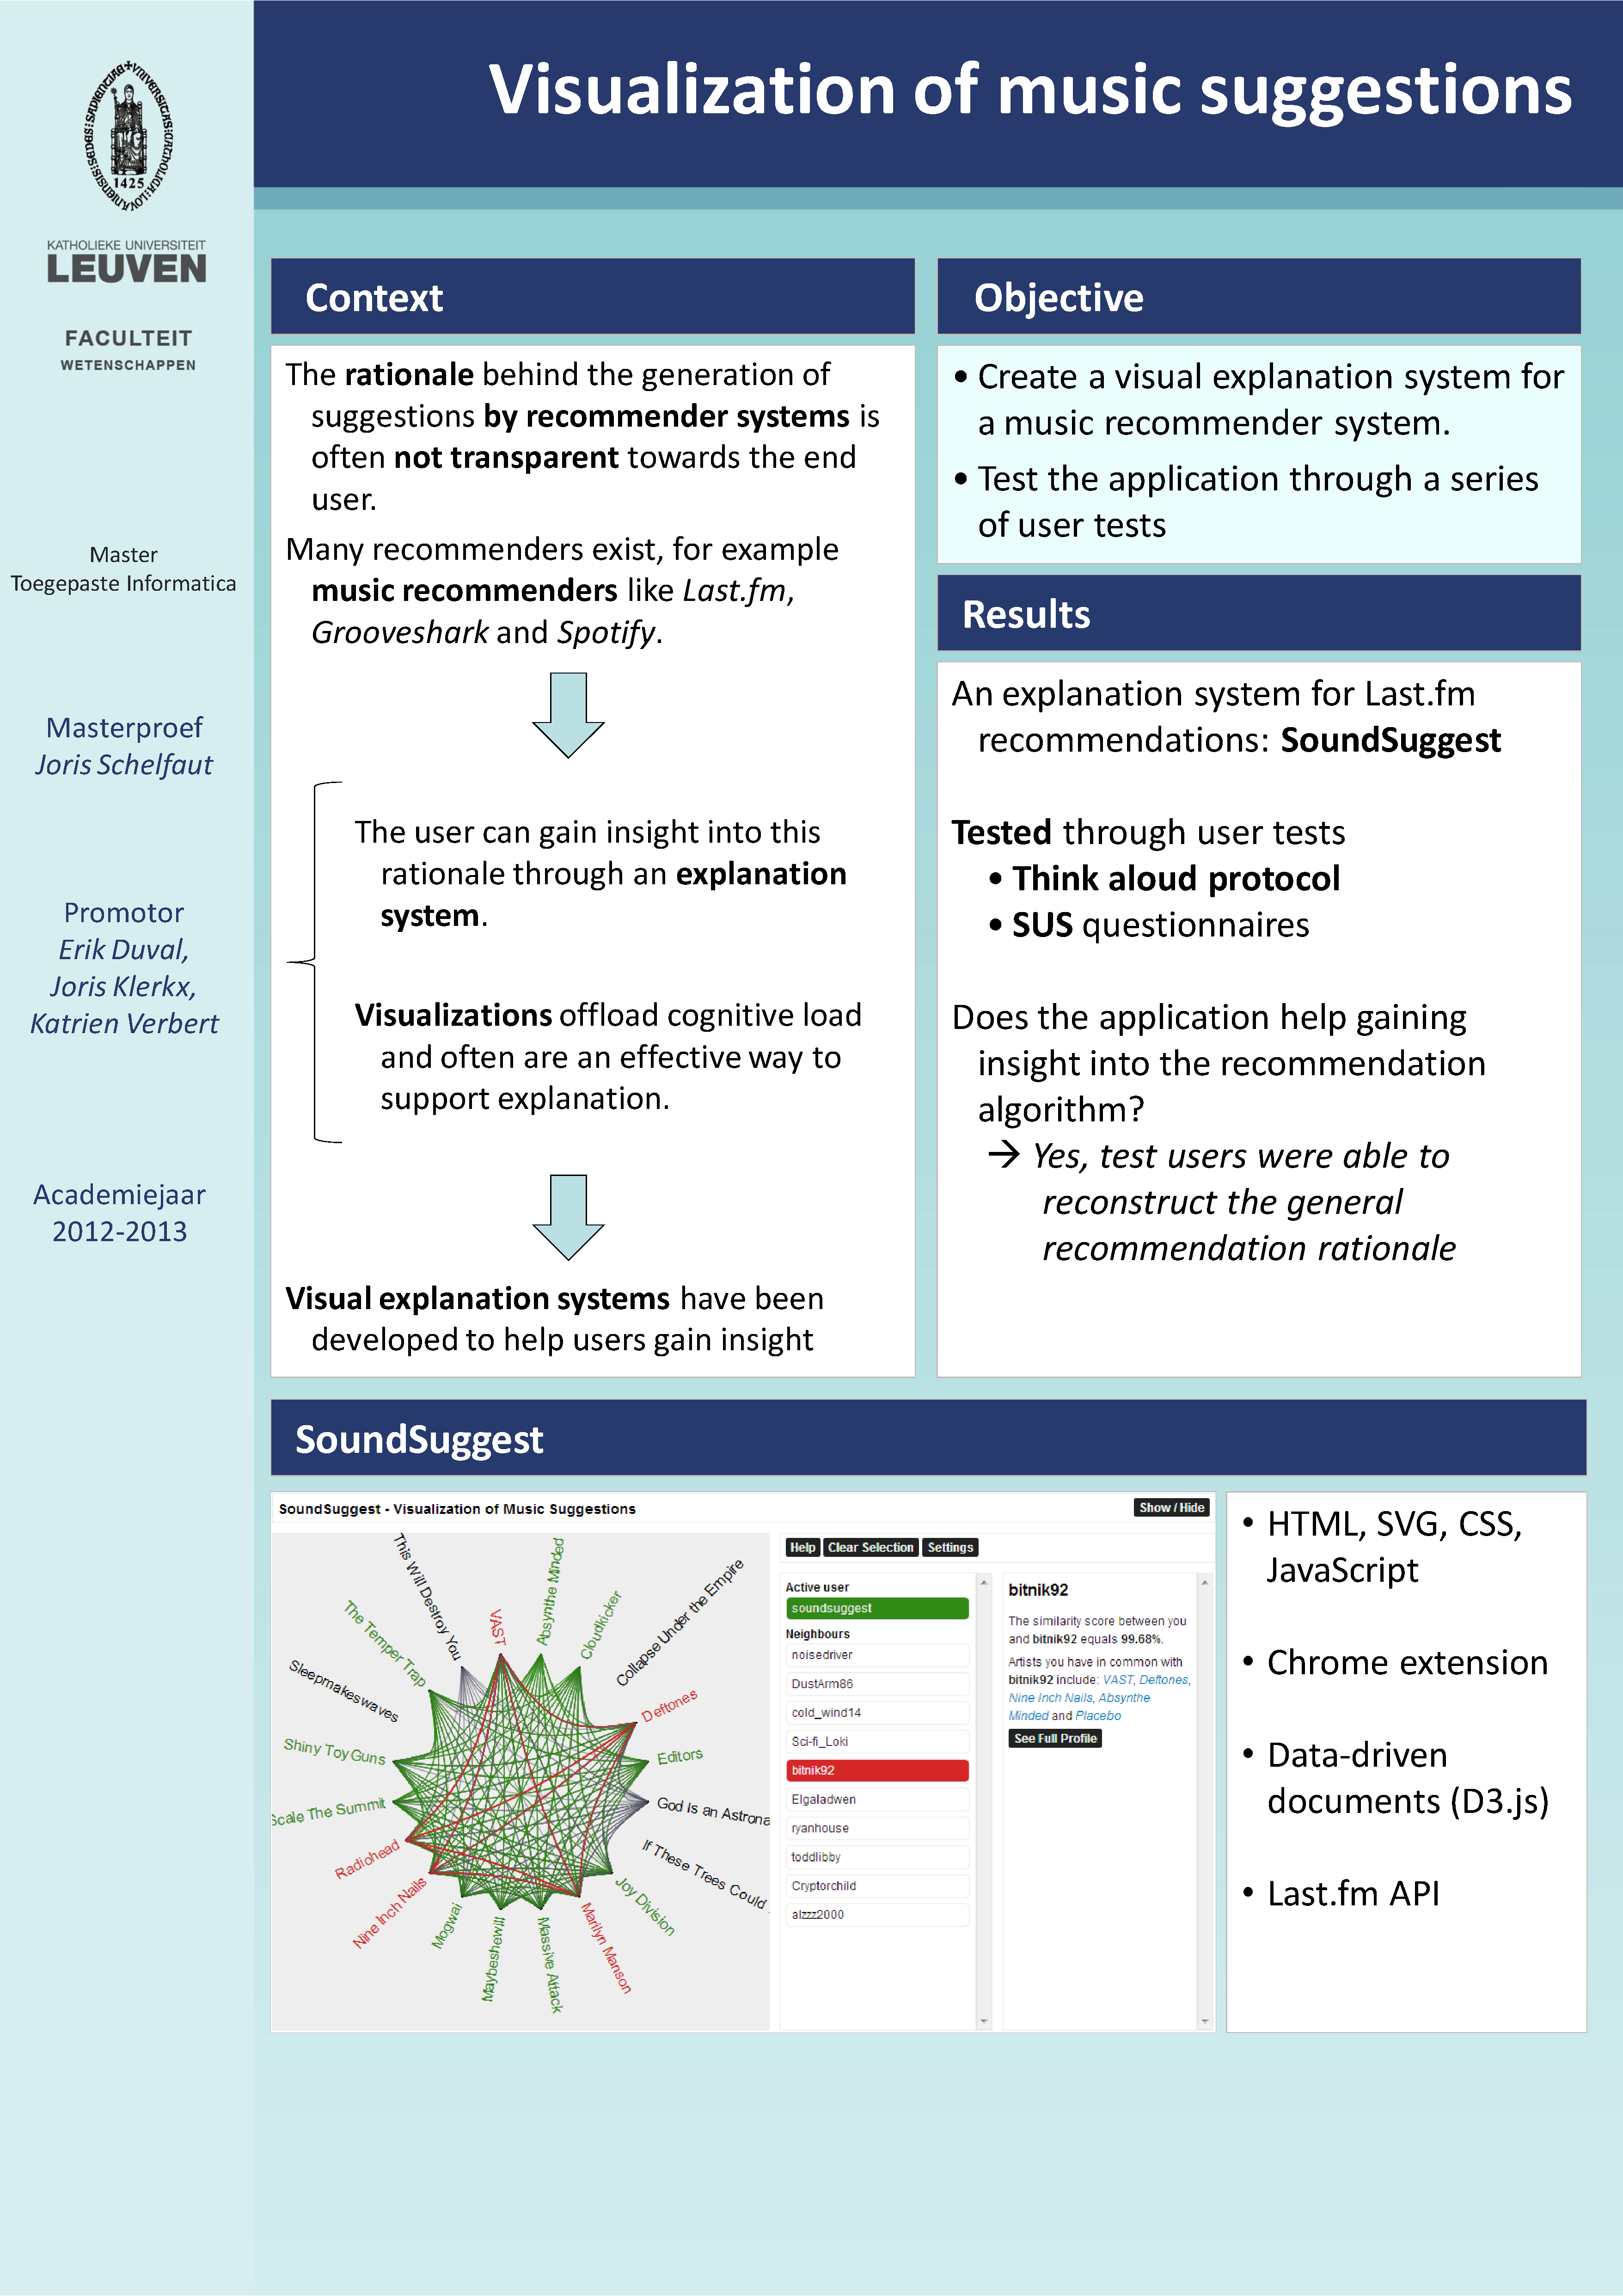
\includepdf[pages={1}]{pdf/poster}


\newpage
% ----------------------- Back cover ------------------------------
% Please fill in:
% - Department
% - Department's address
% - Telephone number and fax number
% - e-mail
% -----------------------------------------------------------------
\thispagestyle{empty}
\sffamily
%
\begin{textblock}{191}(113,-11)
{\color{blueline}\rule{160pt}{5.5pt}}
\end{textblock}
%
\begin{textblock}{191}(168,-11)
{\color{blueline}\rule{5.5pt}{59pt}}
\end{textblock}
%
\begin{textblock}{183}(-24,-11)
\textblockcolour{}
\flushright
\fontsize{7}{7.5}\selectfont
\textbf{AFDELING}\\
Straat nr bus 0000\\
3000 LEUVEN, BELGI\"{E}\\
tel. + 32 16 00 00 00\\
fax + 32 16 00 00 00\\
@kuleuven.be\\
www.kuleuven.be\\
\end{textblock}
%
\begin{textblock}{191}(154,-7)
\textblockcolour{}
\includegraphics*[height=16.5truemm]{sedes}
\end{textblock}
%
\begin{textblock}{191}(-20,235)
{\color{bluetitle}\rule{544pt}{55pt}}
\end{textblock}
\end{document}
